\documentclass[11pt,a4paper,twoside]{tesis}
% SI NO PENSAS IMPRIMIRLO EN FORMATO LIBRO PODES USAR
%\documentclass[11pt,a4paper]{tesis}

\usepackage{multirow}
\usepackage{graphicx}
\usepackage[utf8]{inputenc}
\usepackage[spanish]{babel}
\usepackage[left=3cm,right=3cm,bottom=3.5cm,top=3.5cm]{geometry}
\usepackage{float}
\usepackage{amsmath}
\usepackage{amssymb}
\usepackage{mathtools}
\usepackage{booktabs}
\usepackage{algorithm}
\usepackage[noend]{algpseudocode}
\usepackage{url}
\usepackage{tcolorbox}
\usepackage{subcaption}

\newtcolorbox{wipbox}{
    colback=yellow!10,
    colframe=red!60!black,
    title=WIP,
    fonttitle=\bfseries
}

\newcommand{\mc}[1]{\mathcal{#1}}
\newcommand{\mb}[1]{\mathbf{#1}}
\newcommand{\Exp}{\text{Exp}}
\newcommand{\Log}{\text{Log}}
\newcommand{\wip}[1]
    {
    \begin{wipbox}
        #1
    \end{wipbox}
    }

\makeatletter
\def\BState{\State\hskip-\ALG@thistlm}
\makeatother

\begin{document}

%%%% CARATULA

\def\autor{Jorge Augusto Cevasco Rieck}
\def\tituloTesis{VIGS-Fusion-LC: \vspace{.2cm} \\ Sistema de SLAM visual-inercial basado en Gaussian Splatting con Loop Closure}
%\def\runtitulo{La Guerra de las Galaxias: Rebelión e Imperio}
%\def\runtitle{Star Wars: Rebellion and Empire}
\def\director{Pablo De Cristóforis}
%\def\codirector{Master Yoda}
\def\lugar{Buenos Aires, 2026}

\def\runtitulo{VIGS-Fusion-LC: Sistema de SLAM visual-inercial basado en Gaussian Splatting con Loop Closure}

\input{caratula}

\cleardoublepage
%\begin{center}
%\large \bf \runtitulo
%\end{center}
%\vspace{1cm}
\chapter*{\runtitulo}

\noindent 
En este trabajo se aborda el problema de Localización y Mapeo Simultáneos (SLAM). El objetivo principal fue replicar el trabajo de VIGS-Fusion \cite{ndoye2025vigs}, un sistema de SLAM visual-inercial basado en Gaussian Splatting, y extenderlo incorporando mejoras en la gestión del mapa y añadiendo un hilo dedicado a la detección y cierre de ciclos. 

Para ello, se incorporaron las ideas de FGS-SLAM \cite{xu2025fgsslamfourierbasedgaussiansplatting} en la gestión del mapa, se desarrolló un proceso de detección de ciclos basado en descriptores NetVLAD \cite{arandjelović2016netvladcnnarchitectureweakly} y una optimización global para el cierre de ciclos adaptando el procedimiento propuesto por LoopSplat \cite{zhu2025_loopsplat}.

\bigskip

\noindent\textbf{Palabras claves:} SLAM, Gaussian Splatting, Loop Closure, Procesamiento de Imágenes, Optimización del Grafo de Poses, NetVLAD.

\cleardoublepage
\chapter*{Agradecimientos}

\noindent Quisiera agradecer a mi familia por su apoyo incondicional.

\noindent A mi pareja, por su compañía a lo largo de todo el proceso.

\noindent A mi perrita, por traer alegría a lo largo de toda mi secundaria y carrera universitaria, aunque lamentablemente no haya podido ver esta etapa final. 

\noindent Al profesor Carlos Fuentes, mi primer profesor de la carrera y quien con sus clases dio una gran base a toda mi formación.

\noindent Y a todos los profesores que, en el contexto tan difícil por el que se está pasando, han seguido haciendo un gran esfuerzo para que podamos seguir aprendiendo y manteniendo la calidad educativa que caracteriza esta Facultad.

%%%%%%%%%%%%%%%%%%%%%%%%%%%%%%%%%%%%%
% INTRODUCCION
%%%%%%%%%%%%%%%%%%%%%%%%%%%%%%%%%%%%%
%=========================================================
% CAPÍTULO: Introducción
%=========================================================

\chapter{Introducción}

% --------------------------------------------------
% SECCIONES
% --------------------------------------------------

\section{Motivación}

% Introduccion al problema
La navegación autónoma es un área de investigación activa en robótica, con todo tipo de aplicaciones, desde vehículos autónomos hasta robots de servicio y drones. La capacidad de un robot para navegar de forma segura y eficiente en entornos desconocidos es fundamental para su utilidad y adopción en entornos reales. Esto se logra mediante la construcción de mapas del entorno y la localización del robot dentro de esos mapas, lo que se conoce como \textit{Simultaneous Localization and Mapping} (SLAM). 

A lo largo de la literatura, se han propuesto numerosos algoritmos de SLAM, cada uno con sus propias ventajas y desventajas. Dentro de esos algoritmos, hay un especial interés en aquellos basados en visión, ya que las cámaras son sensores económicos y proporcionan una gran cantidad de información sobre el entorno. Sin embargo, los algoritmos que las utilizan son computacionalmente costosos, lo que limita su aplicación en tareas como la navegacion autónoma, que requieren respuestas a tiempo real.

Una forma de clasificar estos algoritmos es según dos factores: El primero, con qué sensores trabajan, y el segundo, qué tipo de representación del entorno utilizan. Los sensores con los que cuenta el robot determinan la información con la que trabaja el algoritmo, el cual deberá fusionarla entre sí para que brinden resultados más robustos, en un marco de coherencia con la representación del entorno.

% Sensores
En este trabajo se consideran robots equipados con sensores visuales e inerciales, una configuración conocida como VINS (\textit{Visual-Inertial SLAM}). En particular, se empleará una cámara a color junto con un mapa de profundidad por píxel, y una IMU (unidad de medición inercial) que aporta datos de aceleraciones y velocidades angulares en los tres ejes. La información visual permite observar la estructura y la apariencia del entorno, mientras que la IMU entrega medidas de la dinámica del movimiento entre las imágenes, información esencial para mantener estimaciones de pose robustas ante cambios rápidos y en áreas poco texturizadas. La elección de estos sensores se debe a su bajo costo y alta disponibilidad, al igual que a su factibilidad, pues estos sensores son sencillos de integrar y calibrar. Además, su reducido tamaño, requerimiento energético y peso los hacen ideales para plataformas móviles con restricciones de carga útil, como drones o robots de servicio. Sin embargo, la información que aportan es ruidosa y a menudo insuficiente, brindando resultados poco robustos en comparación a la integración de sensores como LiDARs, los cuales son más precisos pero traen consigo un costo mayor en energía, peso y valor monetario.

% Modelo del mundo
Como modelo de mapa, este trabajo adopta la técnica de Gaussian Splatting, surgida recientemente \cite{kerbl2023gaussian}, que ha despertado gran interés por su combinación de calidad y eficiencia de renderizado. En este modelo, el entorno se representa como una colección de gaussianas tridimensionales, cada una con su propia posición, forma y color. Estas gaussianas pueden ser renderizadas de manera eficiente utilizando técnicas de rasterización, lo que permite obtener imágenes de alta calidad a partir de la representación del entorno. Además, el modelo de Gaussian Splatting es capaz de representar detalles finos y texturas complejas, por lo que resulta adecuado para aplicaciones de navegación autónoma en entornos reales. En este modelo, existen distintas técnicas para inicializar y optimizar las gaussianas, surgiendo mucha literatura al respecto.

% VIGS-Fusion / Loop Closure
Dentro del marco de SLAM en el que se ubica este trabajo, artículos recientes exploran distintas formas de integrar los sensores con el modelo de mundo. Tal es el caso de VIGS-Fusion \cite{ndoye2025vigs}, que presenta un algoritmo de SLAM eficiente en tiempo real. Sin embargo, una propiedad que no posee es la que se conoce en la literatura como la detección y cierre de ciclos, que es la capacidad del algoritmo de reconocer lugares previamente visitados y corregir la trayectoria en consecuencia. Del mismo modo, al encontrarse la técnica de Gaussian Splatting en etapas muy tempranas de desarrollo, existe muy poca exploración al respecto, consistiendo mayormente en artículos dispersos orientados a combinaciones específicas de sensores, sin suficiente trabajo en la integración de los resultados entre ellos.



\section{Objetivos}

El objetivo principal de este trabajo el diseño de una variación de VIGS-Fusion \cite{ndoye2025vigs} que integre la detección y cierre de ciclos. Para ello, se exploró la literatura existente sobre los ciclos en el marco de Gaussian Splatting, con énfasis en la implementación de LoopSplat \cite{zhu2025_loopsplat}.

Con estoo en mente, el se realizó una reimplementación de VIGS-Fusion, con el objetivo de mejorar su eficiencia y realizar variaciones a la inicialización de gaussianas. Para esto último, se siguieron otros artículos como FGS-SLAM \cite{xu2025fgsslamfourierbasedgaussiansplatting} y se presentaron variaciones propias.

Además, debido a la falta de literatura completa sobre todo lo que conforma el marco de SLAM con Gaussian Splatting, se realizó un desarrollo exhaustivo en las explicaciones de los conceptos básicos, presentando así una base más completa para futuros trabajos en esta área.



\section{Estructura de la tesis}

En el Capítulo \ref{marco_teorico} se aporta una explicación detallada de todos los conceptos abordados en el marco de este trabajo así como la explicación de los conceptos fundacionales que dan lugar a todas las técnicas. Así, se parte de qué son las imágenes, cómo se forman, qué operaciones se pueden realizar sobre ellas y cómo es que dan lugar a tareas como la visión por computadora y SLAM. Además, se presentan los grupos y álgebras de Lie, así como su integración en SLAM y en el modelo de Gaussian Splatting. Del mismo modo, se describe toda la matemática que resulta necesaria para comprender los sensores y el modelo de Gaussian Splatting trabajados, así como las técnicas de optimización utilizadas.

En el Capítulo \ref{estado_del_arte} se presenta un análisis de los trabajos más relevantes en los que se basa este trabajo.

En el Capítulo \ref{metodo} se brinda una breve explicación de la arquitectura del programa, así como las decisiones de diseño tomadas, complementando la explicación teórica con la forma computacional del algoritmo. Además, se describen de forma minimal los conceptos básicos necesarios para comprender la implementación.

En el Capítulo \ref{resultados} se muestran los resultados obtenidos comparando este trabajo con otros algoritmos de SLAM existentes en la literatura, utilizando distintos conjuntos de datos y las métricas comunes en SLAM.

En el Capítulo \ref{conclusiones} se brindan las conclusiones obtenidas a partir de los resultados, así como las limitaciones del trabajo y las posibles líneas de investigación futura.



%==========================================================


%%%%%%%%%%%%%%%%%%%%%%%%%%%%%%%%%%%%%
% MARCO TEORICO
%%%%%%%%%%%%%%%%%%%%%%%%%%%%%%%%%%%%%
%=========================================================
% CAPÍTULO: MARCO TEÓRICO
%=========================================================

\chapter{Marco Teórico}
\label{marco_teorico}

Este capítulo se introducen los conceptos teóricos necesarios para comprender
los métodos y algoritmos desarrollados en esta tesis. En particular,
se presentan nociones fundamentales relacionadas con la representación
de imágenes digitales, geometría proyectiva, transformaciones rígidas,
grupos y álgebras de Lie, los principios del funcionamiento de sensores inerciales y su relación con el problema de SLAM.

%---------------------------------------------------------
% SECCIONES DEL MARCO TEÓRICO
%---------------------------------------------------------

\section{Notación y convenciones}
\label{sec:notacion}

\subsection{Objetos matemáticos}

\begin{itemize}
	\item Escalares en letra itálica: $\lambda$, $\sigma$, $t$.
	\item Vectores columna en negrita minúscula: $\mathbf{x}$, $\mathbf{v}$, $\mathbf{p}$.
	\item Matrices en negrita mayúscula: $\mathbf{A}$, $\mathbf{R}$, $\mathbf{K}$, $\mathbf{J}$.
	\item Variables aleatorias vectoriales con notación en negrita: $\mathbf{x} \sim \mathcal{N}(\boldsymbol{\mu}, \boldsymbol{\Sigma})$.
	\item Conjuntos, variedades y grupos en caligráfica: $\mathcal{M}$, $\mathcal{G}$, $\mathcal{X}$.
	\item Álgebra de Lie y espacios tangentes en fraktur: $\mathfrak{se}(3)$, $T_{\mathcal{X}}\mathcal{M}$.
\end{itemize}

\subsection{Reglas de escritura}

\begin{itemize}
	\item Los puntos y vectores se tratan como vectores columna.
	\item Las matrices actúan por la izquierda, y la composición se lee de izquierda a derecha según el efecto sobre el objeto.
	\item Los subíndices se usan para enumeración, tiempo, acceso o marco de referencia; los superíndices se reservan para el marco o para indicar cantidades derivadas, según el contexto.
\end{itemize}

\subsection{Covarianzas}

La covarianza se denota siempre con $\boldsymbol{\Sigma}$. Si se requiere la matriz de información, se escribe de forma explícita como
\[
\boldsymbol{\Lambda} \coloneq \boldsymbol{\Sigma}^{-1}.
\]

\subsection{Coordenadas homogéneas, proyección y Jacobiano}

Distinguimos explícitamente entre coordenadas euclídeas y homogéneas. Un punto euclídeo en 3D se denota $\mathbf{p}=\begin{bmatrix}x\\y\\z\end{bmatrix}^\top \in \mathbb{R}^3$, y su representación homogénea se escribe
\[
\tilde{\mathbf{p}} = \begin{bmatrix}\mathbf{p} \\ 1\end{bmatrix} \in \mathbb{R}^4.
\]
La multiplicación por una transformación rígida $\mathbf{T}_{ab}\in SE(3)$ se hace sobre la forma homogénea como se indicó arriba.

Denotamos la operación de proyección desde coordenadas de cámara 3D a coordenadas imagen 2D por $\pi(\cdot)$.

En las derivaciones y en la propagación de incertidumbre usamos la linealización de $\pi$ alrededor de una media $\boldsymbol{\mu}_c$, definida por el Jacobiano
\[
\mathbf{J}_{\pi}(\boldsymbol{\mu}_c) \coloneq \frac{\partial \pi(\mathbf{x}_c)}{\partial \mathbf{x}_c}\Big|_{\mathbf{x}_c=\boldsymbol{\mu}_c} \in \mathbb{R}^{2\times 3}.
\]

En fórmulas concretas del texto usamos notaciones abreviadas como $\mathbf{J}_c$ o $\mathbf{J}_{\pi}$ cuando el contexto identifica claramente la proyección considerada.

\subsection{Transformaciones y marcos}

La notación $\mathbf{T}_{ab}$ denota la transformación que lleva coordenadas expresadas en el marco $a$ al marco $b$. Para un punto homogéneo $\tilde{\mathbf{p}}_a$ se escribe
\[
\tilde{\mathbf{p}}_b = \mathbf{T}_{ab}\,\tilde{\mathbf{p}}_a.
\]
Por lo tanto, la composición se escribe
\[
\mathbf{T}_{ac} = \mathbf{T}_{bc}\,\mathbf{T}_{ab},
\]
si primero se pasa de $a$ a $b$ y luego de $b$ a $c$. 

La transformación inversa es
\[
\mathbf{T}_{ba} = \mathbf{T}_{ab}^{-1}.
\]

\subsection{Operaciones de Lie}

La convención principal de la tesis es la perturbación a derecha. En particular, si $\mathcal{X}, \mathcal{Y} \in \mathcal{G}$ y $\tau \in \mathbb{R}^d$, se define
\[
\mathcal{X} \oplus \tau \coloneq \mathcal{X}\,\Exp(\tau^\wedge),
\qquad
\mathcal{Y} \ominus \mathcal{X} \coloneq \Log\!\left(\mathcal{X}^{-1}\mathcal{Y}\right).
\]
Salvo indicación explícita, se adopta esta convención.

Cuando una formulación provenga de un desarrollo en marco global, la perturbación a izquierda debe escribirse de manera explícita:
\[
\tau \oplus_{\mathrm{izq}} \mathcal{X} \coloneq \Exp(\tau^\wedge)\,\mathcal{X},
\qquad
\mathcal{Y} \ominus_{\mathrm{izq}} \mathcal{X} \coloneq \Log\!\left(\mathcal{Y}\,\mathcal{X}^{-1}\right).
\]

\subsection{Notación auxiliar}

\begin{itemize}
	\item Las medias gaussianas se denotan con $\boldsymbol{\mu}$.
	\item Los residuos se denotan con $\mathbf{r}$ y los Jacobianos con $\mathbf{J}$.
	\item Los vectores de ruido se denotan con letras en negrita, y sus covarianzas con $\boldsymbol{\Sigma}$.
	\item Cuando sea relevante, los vectores unitarios se indicarán con una barra o un acento circunflejo, según el contexto del capítulo.
\end{itemize}


\section{Imágenes y píxeles}

 Una imagen es un tipo de dato discreto que representa una realidad observada en una matriz. En cada posición, se le asigna una representación del color. Estas posiciones podrían tener un valor único en el caso de las imágenes en blanco y negro, o tres valores en caso de las imágenes a color, usualmente RGB (rojo, verde y azul).

Para representar una imagen en términos de la matemática, la consideramos una función $I : \Omega \subset \mathbb{Z}^2 \to \mathbb{R}^c$ tal que mapea coordenadas espaciales $(x,y)$ a valores de intensidad para cada uno de los $c$ canales. Cada canal representa una componente del color, estando los valores en el intervalo $[0,1]$ o en el intervalo de enteros entre $0$ y $255$. El modelo computacional más común es el de una matriz, donde, en orden, se guarda el valor de intensidad de cada píxel en cada canal. En algunos casos, resulta conveniente utilizar una matriz por canal, es decir, teniendo $c$ funciones que devuelven escalares, en lugar de una única función que devuelve un vector de tamaño $c$.

Cada posición de la matriz se conoce como píxel, (del inglés \textit{picture element}). Aunque se los visualiza con frecuencia como cuadrados de colores, los píxeles son muestras puntuales de la realidad, que es continua. Esto nos lleva a que una imagen es una grilla de puntos con espacios vacíos entre ellos. Para no tener esos espacios vacíos, una forma de rellenarlos es usar la información de los píxeles más cercanos para estimar un posible valor para cada punto no muestreado del espacio. A partir del teorema de muestreo de Nyquist-Shannon, sabemos que se puede reconstruir una entidad continua a partir de una discreta usando un filtro de reconstrucción \cite{SmithPixel} bajo ciertas condiciones. En la práctica, los algoritmos de visión por computadora trabajan directamente sobre las imágenes obtenidas por la cámara, pero se fundamentan en la idea de trabajar sobre muestras.

El tamaño de la muestra tomada en la imagen se conoce como resolución, expresada como la cantidad de píxeles en cada dimensión. Por ejemplo, una imagen de $1920 \times 1080$ tiene $1920$ píxeles en la coordenada horizontal y $1080$ en la vertical. La resolución afecta la cantidad de detalles que se pueden capturar en la imagen, así como el tamaño del archivo y el tiempo de procesamiento necesario para analizarla. Por ello, es importante elegir una resolución adecuada, siendo que una resolución alta es más costosa pero trae consigo más información. Cuando la resolución de la imagen es demasiado alta para el procesamiento, se aplican técnicas de muestreo para reducir la resolución, conocidas como \textit{downsampling} o submuestreo.

\begin{figure}[H]
    \centering
    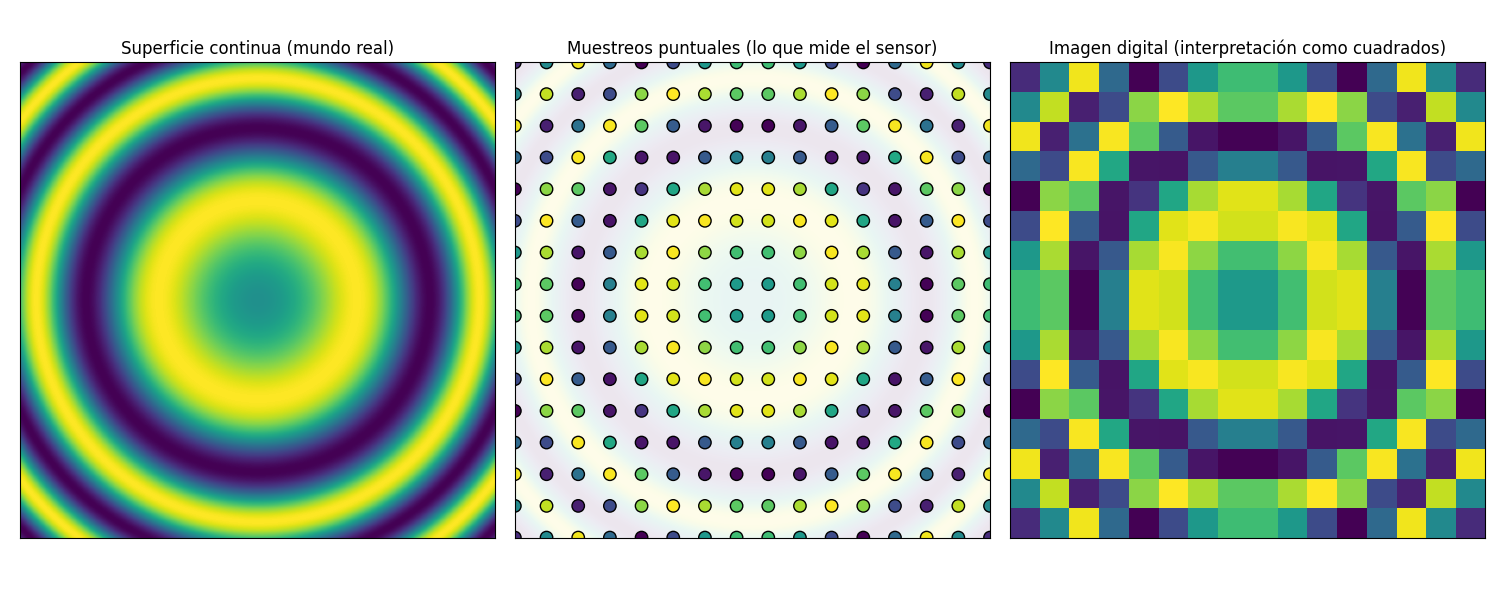
\includegraphics[width=0.7\linewidth, trim = 0cm 0cm 0cm 1.5cm, clip]{../imagenes_marco_teorico/pixel_que_es.png}
    \caption{Se observa a la izquierda una superficie, a la cual se le toma un muestreo en forma de grilla en el centro. Estos puntos son los que se conocen como píxeles. A la derecha, se muestra qué sucede si se interpretan los píxeles como cuadrados, que es la forma usual en la que se observan en computadora.}
    \label{fig:modelo_de_pixel}
\end{figure}

\section{Cámaras y parámetros intrínsecos}

La forma en que los puntos tridimensionales del entorno se relacionan con los píxeles de una imagen tiene que ver con el modelo de cámara en cuestión. En las cámaras estenopeicas (también conocidas como cámaras \textit{pinhole}), modelamos la cámara como una caja donde una de sus paredes tiene un pequeño agujero, que interpretamos como un punto, por el que pasa la luz. La misma incide sobre la pared contraria, donde se ubica una grilla finita de puntos, dando lugar a la imagen. El proceso se conoce como transformación proyectiva.

\begin{figure}[H]
    \centering
    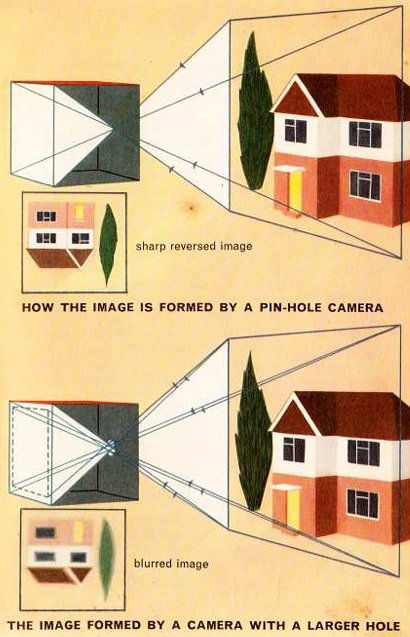
\includegraphics[width=0.5\linewidth]{../imagenes_marco_teorico/matriz_intrinseca.png}
    \caption{Efecto del tamaño del agujero en la proyección. En la parte inferior, la cámara posee un agujero más grande, obteniendo una imagen más borrosa al dejar pasar más luz. Imagen extraida de \cite{howcameraworks}}
    \label{fig:matriz_intrinseca}
\end{figure}

Al pasar por el agujero, la luz se proyecta invertida sobre el plano. Como se observa en la Figura \ref{fig:matriz_intrinseca}, esto sucede al pasar por el agujero, cuya forma, junto a la de la cámara, afectan la imagen resultante. En el modelo, se asume que el agujero es infinitesimalmente pequeño, pero en la práctica eso es físicamente imposible. Por lo tanto, se utilizan lentes que permiten obtener imágenes nítidas al asemejarse al ideal, fijando un punto a través del cual se proyecta la luz, conocido como foco.

Para controlar la diferencia entre el modelo y la realidad, es necesario conocer la geometría de la cámara. En especial, la distancia focal, que es la distancia entre la lente y el foco; y el punto principal, que es la ubicación del píxel de la imagen donde se intersecta el rayo óptico, es decir, el punto donde el centro de la lente se proyecta sobre el plano imagen. En la Figura \ref{fig:lente_grafico11} se muestra una representación de estos parámetros, que resultan fundamentales para modelar la proyección de los puntos sobre la imagen.

\begin{figure}[H]
    \centering
    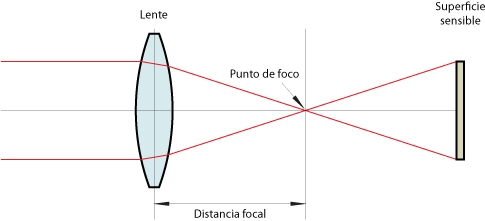
\includegraphics[width=0.5\linewidth]{../imagenes_marco_teorico/lente_grafico11.png}
    \caption{Representación de los parámetros intrínsecos. La superficie sensible es la que recibe la luz para formar la imagen. La línea perpendicular a ella que pasa por el foco es donde se encuentra el punto principal. Imagen extraida de \cite{bokebinario}}
    \label{fig:lente_grafico11}
\end{figure}

Estos parámetros se agrupan en la llamada matriz intrínseca de la cámara, que describe la transformación entre coordenadas del plano de la imagen y coordenadas de píxel del siguiente modo:

\begin{equation}
\mathbf{K} =
\begin{pmatrix}
f_x & 0   & c_x \\
0   & f_y & c_y \\
0   & 0   & 1
\end{pmatrix}
\end{equation}

con $f_x, f_y$ focales en píxeles, y $c_x, c_y$ posición del punto principal. Los valores se pueden obtener a partir de la información del fabricante de la cámara, o mediante un procedimiento de calibración, formalizado en la literatura por Zhang et al. \cite{calibracion_camara}.

\section{Coordenadas homogéneas}

En el contexto de la visión por computadora y la geometría proyectiva, resulta necesario poder representar las llamadas transformaciones afines, que veremos más adelante, y las proyectivas de forma lineal.  Así, se emplea una extensión de las coordenadas euclídeas mediante el uso de coordenadas homogéneas. En las mismas, se agrega una dimensión más al espacio que representa la escala.

Así, un punto bidimensional $(u, v) \in \mathbb{R}^2$ puede representarse en coordenadas homogéneas como el vector
\begin{equation}
    \tilde{\mathbf{u}} =
    \begin{pmatrix}
    u \\
    v \\
    1
    \end{pmatrix},
\end{equation}


mientras que un punto tridimensional $(x, y, z) \in \mathbb{R}^3$ se representa como
\begin{equation}
\tilde{\mathbf{x}} =
\begin{pmatrix}
x \\
y \\
z \\
1
\end{pmatrix}.
\end{equation}

En esta formulación, dos vectores homogéneos que difieren por un factor escalar distinto de cero representan el mismo punto euclídeo. En el caso bidimensional, esto implica que

\begin{equation}
\lambda
\begin{pmatrix}
u \\
v \\
1
\end{pmatrix}
\sim
\begin{pmatrix}
\lambda u \\
\lambda v \\
\lambda
\end{pmatrix},
\qquad \lambda \neq 0,
\end{equation}

Es decir, corresponden a la misma coordenada cartesiana $(u, v)$ luego de normalizar por la última componente.

En el modelo de cámara pinhole, la relación entre un punto del espacio expresado en el sistema de referencia de la cámara y su proyección en la imagen puede escribirse como

\begin{equation}
\lambda
\begin{pmatrix}
u \\
v \\
1
\end{pmatrix}
=
\mathbf{K}
\begin{pmatrix}
x \\
y \\
z
\end{pmatrix},
\end{equation}
donde $\mathbf{K}$ es la matriz intrínseca de la cámara y $\lambda$ es un factor de escala asociado a la profundidad del punto. Este factor es a priori desconocido, y no se puede deducir meramente de una imagen RGB. Si conociéramos $z$, podemos tomar $\lambda = z$, normalizar y obtener que:

\begin{equation}
\begin{pmatrix}
u \\
v \\
1
\end{pmatrix}
=
\mathbf{K}
\begin{pmatrix}
x/z \\
y/z \\
1
\end{pmatrix},
\end{equation}



\section{Transformaciones rígidas y parámetros extrínsecos}
Para poder representar efectivamente el mundo, es necesario un sistema de coordenadas. Para esto, se fija un sistema de coordenadas global, en el cual efectuar transformaciones rígidas. Las mismas son una composición de una rotación y una traslación.

Sea $\mathbf{x}_w \in \mathbb{R}^3$ un punto expresado en el sistema de referencia del mundo.
Su representación en el sistema de la cámara viene dada por

\begin{equation}
\mathbf{x}_c = \mathbf{R}\,\mathbf{x}_w + \mathbf{t},
\end{equation}

donde $\mathbf{R} \in SO(3)$, espacio que trataremos en una sección posterior, es una matriz de rotación, y $\mathbf{t} \in \mathbb{R}^3$ es
un vector de traslación.

Utilizando coordenadas homogéneas, esta relación puede escribirse de forma matricial como

\begin{equation}
\tilde{\mathbf{x}}_c =
\begin{pmatrix}
\mathbf{R} & \mathbf{t} \\
\mathbf{0}^\top & 1
\end{pmatrix}
\tilde{\mathbf{x}}_w.
\end{equation}

Los parámetros $\mathbf{R}$ y $\mathbf{t}$ se conocen como parámetros extrínsecos de la cámara,
ya que describen su posición y orientación en el entorno. Nos referimos a la combinación de ambos como la pose de la cámara.

\section{Proyección}

A partir de los parámetros intrínsecos $\mathbf{K}$ y extrínsecos $\mathbf{R}, \mathbf{t}$ podemos expresar la relación entre un punto ${\mathbf{x}}_w \in \mathbb{R}^3$ y su proyección en el plano imagen $\mathbf{u} \in \mathbb{R}^2$ con una transformación proyectiva del siguiente modo:

\begin{equation}
\lambda \, \tilde{\mathbf{u}} =
\mathbf{K}
\begin{pmatrix}
\mathbf{R} & \mathbf{t}
\end{pmatrix}
\tilde{\mathbf{x}}_w,
\end{equation}

A esta matriz que combina los parámetros intrínsecos y extrínsecos la llamamos $\mathbf{P}$, y, si lo pensamos como una función, la llamamos $\pi$.

En el marco de referencia de la cámara, tenemos puntos de la forma $\mathbf{x}_c = \mathbf{R}\,\mathbf{x}_w + \mathbf{t}$. Al aplicarles las intrínsecas:
\begin{equation}
\pi(\mathbf{x}_w) =
\begin{pmatrix}
u \\
v
\end{pmatrix}
=
\begin{pmatrix}
f_x \dfrac{x_c}{z_c} + c_x \\
f_y \dfrac{y_c}{z_c} + c_y
\end{pmatrix}.
\label{proyeccion_pinhole}
\end{equation}

En particular, nos interesa qué pasa cuando hay pequeñas variaciones en la posición del punto. Para eso, derivamos respecto a cada coordenada para obtener el Jacobiano de la proyección, de ahora en adelante $\mathbf{J}$.
\begin{equation}
\mathbf{J}
=
\frac{\partial \pi(\mathbf{x}_c)}{\partial \mathbf{x}_c}
\in \mathbb{R}^{2 \times 3}.
\end{equation}

Al derivar respecto de $x_c$, $y_c$ y $z_c$, queda

\begin{equation}
\mathbf{J}
=
\begin{pmatrix}
\dfrac{f_x}{z_c} & 0 & -\dfrac{f_x x_c}{z_c^2} \\
0 & \dfrac{f_y}{z_c} & -\dfrac{f_y y_c}{z_c^2}
\end{pmatrix}.
\label{jacobiano_proyeccion_camara}
\end{equation}

Cuando fuere necesario, lo podemos extender a coordenadas homogéneas completando con una fila nula. El uso de una u otra expresión dependerá del contexto del problema.

\begin{equation}
\mathbf{J}_{\mathrm{hom}}
=
\begin{pmatrix}
\dfrac{f_x}{z_c} & 0 & -\dfrac{f_x x_c}{z_c^2} \\
0 & \dfrac{f_y}{z_c} & -\dfrac{f_y y_c}{z_c^2} \\
0 & 0 & 0
\end{pmatrix}.
\end{equation}

\section{Proyección inversa e imágenes de profundidad}

Al capturar una imagen con una cámara, se proyecta un fragmento del espacio sobre un plano. El proceso inverso, en el cual se estima la posición de un punto en el espacio a partir de su proyección en el plano, se llama proyección inversa o \textit{back-projection}. A partir de una imagen particular hay infinitos espacios tridimensionales que podrían reproducirla \cite{ImageReconstruction}. Por ejemplo, dos objetos de las mismas características pero distintos tamaños se podrían ver iguales en imágenes que estén a distinta distancia de la cámara. De este modo, estamos con un problema de inversas que no tiene solución única. 

En \cite{reconstruccion3DConUnaFoto} se aborda este problema con una arquitectura de red de árboles y un autoencoder a partir de una simple imagen RGB. Sin embargo, pese a que es en cierto grado posible agregando supuestos, es un proceso lento y costoso.

Para mejorar el rendimiento, se puede emplear el uso de sensores que producen imágenes de profundidad. Los mismos implementan métodos como \textit{Time of Flight} (ToF), que consiste en medir el tiempo que se tarda en emitir y recibir una luz para cada píxel. La imagen de salida se modela como una función $D: \Omega \subset Z^2 \to \mathbb{R}^+$ tal que para $(x,y)$, tenemos una representación de la distancia entre el centro óptico de la cámara y el punto real de la muestra en el espacio, medida a lo largo del rayo de visión. 

Para renderizarlas, es decir mostrarlas en la pantalla, el resultado puede definirse en una escala. Una posibilidad es en enteros entre 0 y 255, donde 255 representa los puntos que se encuentren más cercanos en la imagen, y 0 los más lejanos. Luego, podemos usar estos valores para obtener una imagen en escala de grises donde un color más claro represente una distancia menor.

\begin{figure}[H]
    \centering
    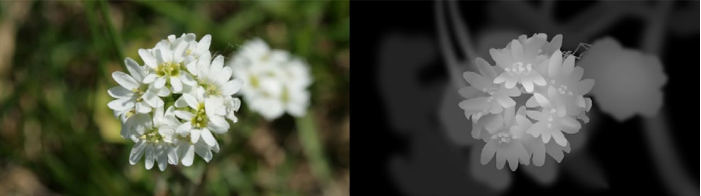
\includegraphics[width=0.8\linewidth]{../imagenes_marco_teorico/imagen_de_profundidad.png}
    \caption{A la izquierda, la imagen RGB, y a la derecha su correspondiente imagen de profundidad. Imagen extraida de \cite{imagen_de_profundidad}}
    \label{prof_imagen}
\end{figure}

En el contexto de este trabajo, se empleó una cámara RGB y una cámara de profundidad, combinación conocida como RGB-D. Debido a esto, no se profundiza en los métodos clásicos basados en la geometría epipolar, que utilizan las imágenes para obtener condiciones sobre los puntos del espacio y así definir mejor el problema. El uso de imágenes de profundidad permite basarse directamente en los datos del sensor para la estimación, a cambio de aceptar cierta cantidad de ruido y error.

Al poseer información de la profundidad, podemos invertir la relación proyectiva para obtener las coordenadas del punto en el sistema de referencia de la cámara:

\begin{equation}
\begin{pmatrix}
x \\
y \\
z
\end{pmatrix}
=
z \, \mathbf{K}^{-1}
\begin{pmatrix}
u \\
v \\
1
\end{pmatrix}.
\end{equation}

De este modo, cada píxel con información de profundidad puede asociarse a un punto
tridimensional expresado en el sistema de la cámara. Es decir, queda definido el $\lambda$ que antes desconocíamos, y el problema de inversas queda resuelto. Sin embargo, la reconstrucción sigue afectada por otros factores como el ruido, las oclusiones, y la observación incompleta del entorno. Además, desconociendo la pose de la cámara no es posible llevar la reconstrucción a coordenadas globales.

\section{Reconstrucción a partir de múltiples imágenes y odometría}

Al capturar un mismo entorno desde diversas imágenes distintas, tenemos un nuevo tipo de problema. Ahora, tenemos mucha más información espacial, que depende para cada imagen tanto de la región capturada como de la pose de la cámara.

\begin{figure}[H]
    \centering
    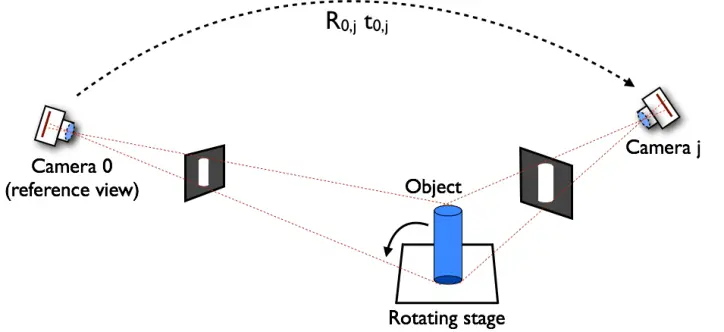
\includegraphics[width=1\linewidth]{../imagenes_marco_teorico/multiples_imagenes.png}
    \caption{Un mismo objeto capturado desde dos puntos. Las cámaras se diferencian por su pose. Imagen extraída de \cite{multiview_reconstruction_blog}.}
    \label{fig:multiview_reconstruction}
\end{figure}

Cada cámara tiene su propia rotación $\mathbf{R}$ y traslación $\mathbf{t}$, no están ordenadas y no tienen necesariamente los mismos parámetros intrínsecos. En la figura \ref{fig:multiview_reconstruction}, se observa este problema fijando una cámara como referencia y teniendo que encontrarse los parámetros de las demás respecto de la inicial. El abordaje de este problema se conoce como \textit{Structure from Motion} (SfM), tratado comúnmente de forma offline y con gran costo computacional. En la figura \ref{fig:rome16k} se observa un ejemplo de este tipo de reconstrucción a gran escala.

\begin{figure}[H]
    \centering
    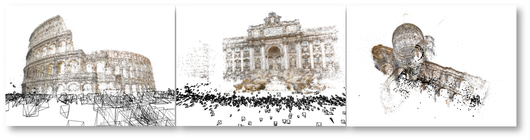
\includegraphics[width=1\linewidth]{../imagenes_marco_teorico/rome16k.png}
    \caption{Las más de dos millones de fotografías de edificios de Roma dieron lugar a un proyecto de reconstrucción llamado \textit{Building Rome in a Day}, llevando a gran escala la SfM. Imágenes extraídas de \cite{building_rome_agarwal}.}
    \label{fig:rome16k}
\end{figure}

Debido a la naturaleza de las imágenes a color, además, el mapa reconstruido no tiene ninguna noción de la escala real de los objetos. Esto se debe a que una imagen a color presenta una ambigüedad respecto a la distancia: por ejemplo de si se trata de un objeto cercano muy chico, o un objeto lejano muy grande \cite{sfm_scale_ambiguity}, como mencionamos anteriormente. Para tratar este problema, es necesario añadir información extra, por ejemplo fusionando la imagen a color con la información de otros sensores. En el marco de este trabajo, el mantenimiento de la escala real resulta crucial, y es gracias a las imágenes RGB-D que se elimina esta ambigüedad. Sin embargo, ambas cámaras están separadas en el espacio, por lo que resulta necesario un paso previo para fusionar las imágenes en una sola, alineando sus datos. Este proceso se conoce como registro.

Para ello, elegimos uno de los marcos relativos para expresar la imagen resultante. En este caso, el marco de la cámara a color, por lo que necesitamos registrar la profundidad. Luego, necesitamos datos previos sobre las intrínsecas de ambas cámaras, y las extrínsecas que llevan de una cámara a la otra. Con todo esto, una vez tomamos una imagen a color y una de profundidad, utilizamos la proyección inversa con las intrínsecas de la cámara de profundidad para llevar los puntos bidimensionales desde el plano de la cámara de profundidad hacia el espacio, expresado en el marco de esta misma cámara. Luego, con las extrínsecas pasamos hacia el marco de la cámara de color transformando todos los puntos, tras lo cual utilizamos los datos de las intrínsecas para pasar al plano de la cámara a color. Este procedimiento se observa en la figura \ref{fig:rgbd_registration}.

\begin{figure}[H]
    \centering
    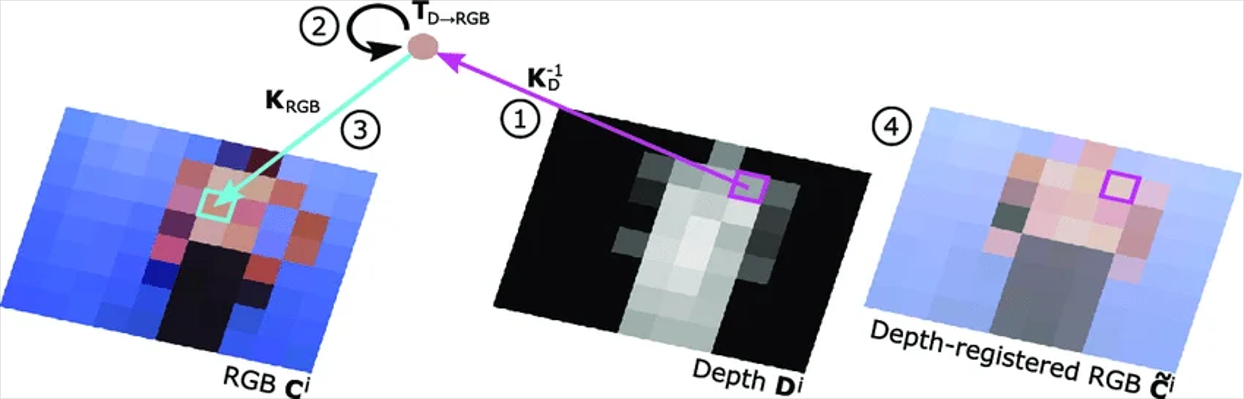
\includegraphics[width=0.75\linewidth]{../imagenes_marco_teorico/rgbd_registration.png}
    \caption{Registrado de un píxel particular, usando las intrínsecas $\mathbf{K}$ y extrínsecas $\mathbf{T}$. Imagen extraída de \cite{rgbd_registration}.}
    \label{fig:rgbd_registration}
\end{figure}



\section{Localización y mapeo simultáneos}

El marco de nuestro trabajo abordó una versión distinta de este problema, ampliamente utilizada en el área de la robótica. Tomamos imágenes a tiempo real, las ordenamos bajo el criterio temporal, y nos interesa obtener tanto la reconstrucción del entorno, llamado mapeo, como la localización de la cámara, llamada pose, a lo largo de la secuencia. Nos encontramos con el problema de \textit{Simultaneous Localization and Mapping} (SLAM).

Hay dos estrategias empleadas para encarar el problema, que son la indirecta y la directa. En la primera, se pre-procesan los datos básicos de los sensores para obtener representaciones intermedias más concretas centrándose en \textit{features} o puntos clave, mientras que en la segunda se usan los datos directamente. Estos últimos tienden a ser más costosos, pues tienen que encarar el problema para todos los puntos de la imagen; sin embargo, se vuelven más precisos gracias a ello. En particular, la literatura emplea algoritmos paralelizables para poder implementar en la Unidad de Procesamiento de Gráficos (GPU).

El planteamiento clásico de SLAM se formula en un marco probabilístico, modelando el problema mediante grafos de factores y buscando el \emph{maximum a posteriori} (MAP) de la distribución de probabilidad conjunta. Dado un estado inicial del robot $\mathbf{x}_0$, un conjunto de controles $\mathbf{u}_{0:T-1}$ y mediciones sensoriales $\mathbf{z}_{1:T}$, el objetivo es estimar la trayectoria de estados $\mathbf{x}_{1:T}$ y el mapa $\mathbf{m}$ que mejor expliquen las observaciones.

Bajo supuestos habituales de ruido gaussiano e independencia condicional de los errores de los sensores, el problema puede expresarse como la minimización de una suma de errores cuadráticos:
\begin{equation}
\min_{\mathbf{x}_{1:T},\,\mathbf{m}}
\sum_{t=1}^{T}
\big\|
\mathbf{z}_t - h(\mathbf{x}_t, \mathbf{m})
\big\|_2^2
\;+\;
\sum_{t=0}^{T-1}
\big\|
\mathbf{x}_{t+1} - f(\mathbf{x}_t, \mathbf{u}_t)
\big\|_2^2,
\end{equation}
donde $h(\cdot)$ denota el modelo de observación, que predice la medición esperada a partir del estado y el mapa, y $f(\cdot)$ representa el modelo de movimiento del sistema. Esta formulación conduce naturalmente a una estructura de grafo dispersa, en la cual cada término del costo corresponde a un factor que conecta un subconjunto reducido de variables.

Este enfoque permite resolver el problema de SLAM mediante técnicas de optimización no lineal y factorización de matrices dispersas, constituyendo la base de numerosos sistemas modernos de SLAM.

Otro enfoque posible es el de interpretar el modelo de observación como un renderizador que, a partir de un mapa tridimensional y una pose de la cámara, genera una imagen artificial. Así, el objetivo es encontrar las variables que minimicen la diferencia entre la imagen renderizada y la real. Este enfoque permite crear variables que representen el entorno de distintas formas, como una nube de puntos \cite{Sandström2023ICCV}, de voxels \cite{liu2024voxelslamcompleteaccurateversatile} o de triángulos (\textit{meshes}) \cite{10161425}. Otras representaciones, muy empleadas en la literatura, son las que se caracterizan por ser tanto continuas como diferenciables, permitiendo el uso de optimización por gradientes. Tal es el caso de NeRF y Gaussian Splatting. Todos estos métodos hacen fuerte uso de las propiedades pertenecientes a los grupos de Lie para poder formular y derivar sus ecuaciones fundamentales y expresar los errores a optimizar.


\section{Grupos y álgebras de Lie}

La teoría de Lie, llamada incluso un milagro en \cite{stillwell2008naive}, es una de las formalizaciones matemáticas más fuertes para la robótica en la literatura actual, aunque su alcance es mucho mayor. Con esta teoría, se permite modelar los estados, las medidas y las funciones que las relacionan, así como sus errores. 

Debido a que en el marco de la odometría visual no se emplean todas las herramientas de la teoría de Lie, nos limitamos a explicar la pequeña parte que es utilizada en el desarrollo posterior.

La idea fundamental de esta teoría es que un estado pertenece a un espacio que cumple ser cierto tipo de variedad o \textit{manifold}, y ser grupo, dando lugar a un grupo de Lie. Estos grupos de Lie pueden ser no euclídeos, inutilizando muchas de las herramientas matemáticas usuales. Mediante la teoría de Lie, sin embargo, se desarrolla una relación con un espacio lineal.

A partir de esta relación, dado un elemento del grupo, se puede encontrar para cada punto en su entorno un equivalente en el álgebra, que es un espacio tangente a la identidad del grupo. Luego podemos realizar todas las operaciones que fuesen necesarias aprovechando la linealidad de este espacio, para obtener un nuevo punto de interés, el cual, por la relación, tendrá un equivalente que permite volver al grupo de Lie. 

Para esta sección, seguiremos de cerca los apuntes de \cite{sola2021microlietheorystate}.

%%%%%%%%%%%%%%%%%%%%%%%%%%%%%%%%%%%%%%%%%%%%%%%%%%%%%%%%%%%%%%%%%%%%%%%%%%%

\subsection{Grupos de Lie}

Un grupo de Lie $\mathcal{G}$ es un conjunto que satisface dos propiedades: Es un grupo con operación suave, y es una variedad suave.

Una variedad suave es un espacio topológico que, localmente, se asemeja a un espacio lineal. Es suave en el sentido de diferenciable, por lo que, dicho de forma más sencilla, no tiene bordes ni picos. Este espacio suele encontrarse dentro de otro espacio bajo ciertas restricciones de estado. Tal es el caso de los vectores en $\mathbb{R}^3$ que cumplen con tener norma uno. Este espacio conforma una variedad esférica de radio uno y suave.

Un grupo $(\mathcal{G}, \circ)$ es un conjunto $\mathcal{G}$ con una operación de composición $\circ$, tal que satisface los siguientes axiomas:

Dados $\mathcal{X}, \mathcal{Y}, \mathcal{Z} \in \mathcal{G}$ cualesquiera,

\begin{enumerate}
\item \textbf{Clausura:} 
Para todo $\mathcal{X}, \mathcal{Y} \in \mathcal{G}$,
\[
\mathcal{X} \circ \mathcal{Y} \in \mathcal{G}.
\]

\item \textbf{Elemento neutro:} 
Existe un elemento $\mathcal{E} \in \mathcal{G}$ tal que, para todo $\mathcal{X} \in \mathcal{G}$,
\[
\mathcal{E} \circ \mathcal{X} = \mathcal{X} \circ \mathcal{E} = \mathcal{X}.
\]

\item \textbf{Elemento inverso:} 
Para todo $\mathcal{X} \in \mathcal{G}$ existe un elemento inverso $\mathcal{X}^{-1} \in \mathcal{G}$ tal que
\[
\mathcal{X}^{-1} \circ \mathcal{X}
=
\mathcal{X} \circ \mathcal{X}^{-1}
=
\mathcal{E}.
\]

\item \textbf{Asociatividad:} 
Para todo $\mathcal{X}, \mathcal{Y}, \mathcal{Z} \in \mathcal{G}$,
\[
(\mathcal{X} \circ \mathcal{Y}) \circ \mathcal{Z}
=
\mathcal{X} \circ (\mathcal{Y} \circ \mathcal{Z}).
\]
\end{enumerate}

En todos los puntos del grupo de Lie, los espacios tangentes se ven igual relativo al punto en cuestión, es decir, son isomorfos. En particular, hay un elemento del grupo que es la identidad, la cual tiene su propio espacio tangente que llamamos el álgebra de Lie del grupo de Lie.


%%%%%%%%%%%%%%%%%%%%%%%%%%%%%%%%%%%%%%%%%%%%%%%%%%%%%%%%%%%%%%%%%%%%%%%%%%%

\subsection{Acciones de grupo}

Con los grupos de Lie, es posible transformar elementos de otros conjuntos, como rotaciones o escalas, o combinaciones de transformaciones.

Dado un Grupo de Lie $\mathcal{M}$ y un conjunto $\mathcal{V}$, se nota $\mathcal{X} \cdot v$ a la acción de $\mathcal{X} \in \mathcal{M}$ en $v \in \mathcal{V}$,

$$
\cdot : \mathcal{M} \times \mathcal{V} \to \mathcal{V}, 
\qquad
(\mathcal{X}, v) \mapsto \mathcal{X} \cdot v.
$$

Para que $\cdot$ sea una acción de grupo, tiene que satisfacer los siguientes axiomas:

\begin{enumerate}
\item \textbf{Identidad:}  
Existe un elemento identidad $\mathcal{E} \in \mathcal{M}$ tal que, para todo $v \in \mathcal{V}$,
\[
\mathcal{E} \cdot v = v.
\]

\item \textbf{Compatibilidad con la composición:}  
Para todo $\mathcal{X}, \mathcal{Y} \in \mathcal{M}$ y todo $v \in \mathcal{V}$,
\[
(\mathcal{X} \circ \mathcal{Y}) \cdot v
=
\mathcal{X} \cdot (\mathcal{Y} \cdot v).
\]
\end{enumerate}

Podemos pensar la composición $\circ$ como un caso particular de acción del grupo a sí mismo.


%%%%%%%%%%%%%%%%%%%%%%%%%%%%%%%%%%%%%%%%%%%%%%%%%%%%%%%%%%%%%%%%%%%%%%%%%%%

\subsection{Álgebra de Lie}

Denotamos el espacio tangente a un punto $\mathcal{X} \in \mathcal{M}$ como $T_{\mathcal{X}} \mathcal{M}$.

En particular, el espacio tangente a la identidad, $\mathcal{T_E M}$ es llamado el álgebra de Lie de $\mathcal{M}$, notado $\mathfrak{m}$.

Es importante mencionar que $\mathfrak{m}$ es un espacio vectorial de dimensión igual a los grados de libertad de $\mathcal{M}$. En la literatura, se nota a elementos del álgebra de Lie con $\wedge$, como $v^\wedge$ para velocidades. También se añade un identificador en la esquina superior izquierda cuando se quiere especificar el espacio tangente en cuestión, por ejemplo, $^{\mathcal{X}}v^\wedge$. 

La estructura del espacio tangente se puede obtener diferenciando la restricción del grupo del siguiente modo: tomamos una curva parametrizada en el tiempo y la recorremos. La diferenciación representa derivar la curva, ya que resulta tangente a la variedad. Además, a partir de ello distinguimos un caso particular: los grupos multiplicativos inducen una restricción adicional, que es 
$$
\mathcal{X}^{-1} \mathcal{\dot{X}} + \mathcal{\dot{X}}^{-1}\mathcal{X} = 0.
$$

Así, los elementos del álgebra de Lie, es decir del espacio tangente a la identidad, son de la forma

\begin{equation}
v^{\wedge} = \mathcal{X}^{-1} \mathcal{\dot{X}} = - \mathcal{\dot{X}}^{-1} \mathcal{X}
\label{derivada_algebra_lie}
\end{equation}

Los elementos del álgebra de Lie, notados $\tau^{\wedge}$, pueden ser expresados como combinación lineal de una base $E$ de $\mathfrak{m}$. Los elementos $E_i$ son llamados generadores y son las derivadas de $\mathcal{X}$ alrededor del origen para cada dirección $i$. 

De esta forma, podemos manipular las coordenadas como vectores en $\mathbb{R}^{m}$, con $m$ la dimensión de $\mathfrak{m}$, las cuales denotaremos $\tau$. Podemos pasar entre $\mathfrak{m}$ y $\mathbb{R}^{m}$ mediante dos isomorfismos que se llamaran $hat$ y $vee$, que son uno la inversa del otro.

$$
\text{Hat:}\quad
\mathbb{R}^m \to \mathfrak{m}, \qquad
\tau \mapsto \tau^\wedge = \sum_{i=1}^m \tau_i E_i,
$$

$$
\text{Vee:}\quad
\mathfrak{m} \to \mathbb{R}^m, \qquad
\tau^\wedge \mapsto (\tau^\wedge)^\vee = \tau = \sum_{i=1}^m \tau_i \mathbb{e}_i,
$$

donde $\mathbf{e}_i$ son los vectores de la base de $\mathbb{R}^m$, con $\mathbf{e}_i^\wedge = E_i$.

Con estos isomorfismos, se vuelve conveniente trabajar directamente en $\mathbb{R}^m$, pues permite utilizar operaciones matriciales y herramientas del cálculo de forma más sencilla.

%%%%%%%%%%%%%%%%%%%%%%%%%%%%%%%%%%%%%%%%%%%%%%%%%%%%%%%%%%%%%%%%%%%%%%%%%%%


\subsection{Mapa exponencial y mapa inverso}

Llamamos retracción al mapeo de elementos del álgebra de Lie hacia el grupo. Esto se hace a partir de una función que se conoce como mapa exponencial, función exponencial o aplicación exponencial $\exp()$. La misma envuelve el espacio tangente sobre la variedad sobre la geodésica, que es el arco mínimo. Análogamente, el mapa inverso $\log()$ desenvuelve el mapeo para mapear posiciones de la variedad a posiciones del espacio tangente.



\begin{figure}[H]
    \centering
    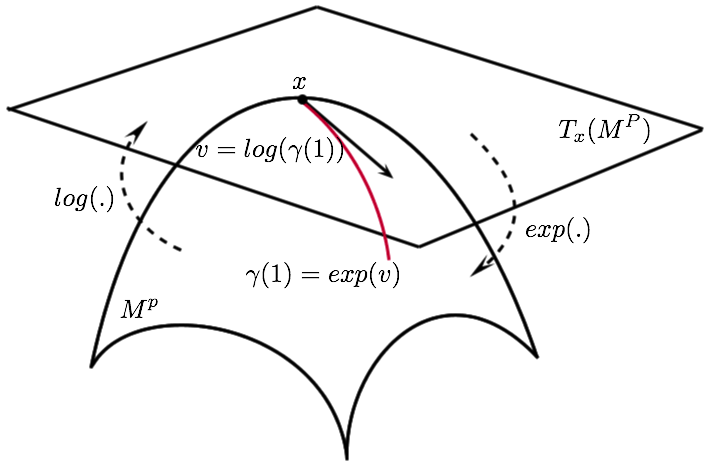
\includegraphics[width=0.75\linewidth]{../imagenes_marco_teorico/mapa_exponencial.png}
    \caption{El espacio tangente en $\mathbf{x}$, lineal, se transforma a partir del mapa exponencial para envolver la variedad. En el vector negro y la curva roja se observa cómo se recorre la variedad desde $\mathbf{x}$, por la geodésica. Imagen extraída de \cite{simeoni2013statistics}.}
    \label{grafico_mapa_exponencial}
\end{figure}

El mapa exponencial surge al considerar las derivadas temporales de $\mathcal{X} \in \mathcal{M}$ sobre la variedad. Despejando la ecuación \ref{derivada_algebra_lie}, tenemos que

$$
\mathcal{\dot{X}} = \mathcal{X} v^\wedge
$$

Fijando $v$, tenemos una Ecuación Diferencial Ordinaria de solución
$$
\mathcal{X}(t) = \mathcal{X}(0) \exp(v^\wedge t)
$$

Como $\mathcal{X}(t)$ y $\mathcal{X}(0)$ son elementos del grupo, entonces $\exp(v^\wedge t) = \mathcal{X}(0)^{-1} \mathcal{X}(t)$ lo es también. Luego, $\exp(v^\wedge t) $ mapea elementos $v^\wedge$ del álgebra de Lie al grupo.

Para los grupos multiplicativos, se puede obtener una forma cerrada del mapa exponencial mediante el desarrollo de Taylor:

\begin{equation}
\exp(\tau^\wedge) = \mathcal{E} + \tau^\wedge + \frac{1}{2} {\tau^\wedge}^2 +
                        \frac{1}{3!} {\tau^\wedge}^3 + \cdot \cdot \cdot
\end{equation}

El mapa exponencial cumple las siguiente propiedades:

\begin{itemize}

\item $\exp((t+s)\tau^\wedge) = \exp(t \tau^\wedge) \exp(s\tau^\wedge)$
\item $\exp(t\tau^\wedge) = \exp(\tau^\wedge)^t$
\item $\exp(-\tau^\wedge) = \exp(\tau^\wedge)^{-1}$
\item $\exp(\mathcal{X} \tau^\wedge \mathcal{X}^{-1}) = \mathcal{X} \exp(\tau^\wedge) \mathcal{X}^{-1}$

\end{itemize}

Del mismo modo que podemos hablar del mapa exponencial e inverso, podemos hablar de la versión en mayúscula Exp y Log, que comprimen mapear directamente vectores a puntos de la variedad, y viceversa.

\begin{figure}[H]
    \centering
    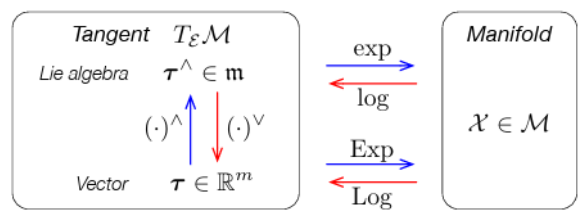
\includegraphics[width=0.6\linewidth]{../imagenes_marco_teorico/mapeo_exponencial_2.png}
    \caption{Se puede observar la relación entre todos los operadores definidos y cómo viajan entre el espacio tangente y la variedad. Imagen extraída de \cite{sola2021microlietheorystate}.}
\end{figure}

\subsection{Suma y Resta directas}

Mediante la suma y resta podemos analizar incrementos en una variedad expresándolos en el espacio lineal a partir de los operadores Exp y Log. Como la composición no es conmutable, definimos a izquierda y a derecha según el orden de los operandos.

\begin{itemize}
\item 
$$
\oplus \text{ a derecha}: \qquad \mathcal{Y} = \mathcal{X} \oplus \\^\mathcal{X}\tau \coloneq
                    \mathcal{X} \circ \text{Exp}(^\mathcal{X}\tau) \in \mathcal{M}
$$

\item
$$
\ominus \text{ a derecha}: \qquad ^\mathcal{E}\tau = \mathcal{Y} \ominus \mathcal{X} \coloneq
             \text{Log}(\mathcal{X}^{-1} \circ \mathcal{Y}) \in \mathcal{T}_\mathcal{X}\mathcal{M}
$$

\item 
$$
\oplus \text{ a izquierda}: \qquad \mathcal{Y} = \\^\mathcal{X}\tau \oplus \mathcal{X} \coloneq
                    \text{Exp}(^\mathcal{E}\tau) \circ \mathcal{X} \in \mathcal{M}
$$

\item 
$$
\ominus \text{ a izquierda}: \qquad ^\mathcal{E}\tau = \mathcal{Y} \ominus \mathcal{X} \coloneq
             \text{Log}(\mathcal{Y} \circ \mathcal{X}^{-1}) \in \mathcal{T}_\mathcal{E}\mathcal{M}
$$

\end{itemize}

Notemos que en la suma directa varía el orden de los operandos, pero en la resta directa no queda claro. Para subsanar el abuso de notación, por defecto se usan las formas a derecha de ambos operadores, a menos que se indique lo contrario. Es decir, utilizaremos las versiones locales.

La forma intuitiva es que la suma directa se encarga de aplicar un movimiento incremental, mientras que la resta directa devuelve qué movimiento incremental llevaría de un punto a otro.

\subsection{Adjunta y Matriz Adjunta}

Igualando la suma a izquierda y a derecha, y utilizando las propiedades antes descritas, tenemos que:
    
\begin{equation}
\begin{split}
\prescript{\mathcal{E}}{}{\tau} \oplus \mathcal{X} &= \mathcal{X} \oplus \prescript{\mathcal{X}}{}{\tau} \\\\
 %
\text{Exp}(\prescript{\mathcal{E}}{}{\tau}^\wedge) \mathcal{X} &= 
\mathcal{X} \text{Exp}(\prescript{\mathcal{X}}{}{\tau})
\\\\
%
\exp(\prescript{\mathcal{E}}{}{\tau}\mathcal{X}) =
\mathcal{X} &\exp(\prescript{\mathcal{X}}{}{\tau})^\wedge \mathcal{X}^{-1} = 
\exp(\mathcal{X} \prescript{\mathcal{X}}{}{\tau}^\wedge \mathcal{X}^{-1}) \\\\
 %
\prescript{\mathcal{E}}{}{\tau}^\wedge &= 
\mathcal{X} \prescript{\mathcal{X}}{}{\tau}^\wedge \mathcal{X}^{-1}
\end{split}
\end{equation}

A partir de esto, se define la adjunta de $\mc{M}$ en $\mc{X}$ del siguiente modo:

$$
\text{Ad}_\mc{X} : \mathfrak{m} \to \mathfrak{m}; \qquad
\tau^\wedge \mapsto \text{Ad}_\mc{X}(\tau^\wedge) \coloneq
\mc{X} \tau^\wedge \mc{X}^{-1}
$$

De este modo $\prescript{\mc{E}}{}{\tau}^\wedge = \text{Ad}_\mc{X}(\prescript{\mc{X}}{}{\tau}^\wedge)$, que llamamos la acción adjunta del grupo en su álgebra de Lie.

Debido a que la adjunta es lineal, se define un operador matricial equivalente:

$$
\textbf{Ad}_\mc{X} : \mathbb{R}^m \to \mathbb{R}^m; \qquad
\prescript{\mc{X}}{}{\tau} \mapsto \prescript{\mc{E}}{}{\tau} = 
\textbf{Ad}_\mc{X} (\prescript{\mc{X}}{}{\tau})
$$

llamado matriz adjunta. Se obtiene de aplicar el operador Vee a la adjunta

$$
\textbf{Ad}_\mc{X}(\tau) = (\mc{X} \tau^\wedge \mc{X}^{-1})^\vee
$$

Algunas propiedades son:

\begin{itemize}
    \item
    $$
    \mc{X} \oplus \tau = (\textbf{Ad}_\mc{X} \tau) \oplus \mc{X}
    $$
    \item 
    $$
    \textbf{Ad}_{\mc{X}^{-1}} = \textbf{Ad}_{\mc{X}}^{-1}
    $$
    \item 
    $$
    \textbf{Ad}_{\mc{X}\mc{Y}} = \textbf{Ad}_\mc{X} \textbf{Ad}_\mc{Y}
    $$
\end{itemize}

%%%%%%%%%%%%%%%%%%%%%%%%%%%%%%%%%%%%%%%%%%%%%%%%

\subsection{Derivadas y Jacobianos}

Para definir las incertidumbres y los incrementos, se emplea una definición análoga al Jacobiano clásico del análisis. 

Dada una función $f: \mathbb{R}^m \to \mathbb{R}^n$, su Jacobiano es

$$
\mc{J}
=
\frac{\partial f(x)}{\partial x}
=
\begin{bmatrix}
\frac{\partial f_1}{\partial x_1} & \cdots & \frac{\partial f_1}{\partial x_m} \\
\vdots & \ddots & \vdots \\
\frac{\partial f_n}{\partial x_1} & \cdots & \frac{\partial f_n}{\partial x_m}
\end{bmatrix}
\in \mathbb{R}^{n \times m}.
$$

Si lo particionamos en vectores columnas $j_i$ para $i = 1,2,...,m$,

$$
j_i = \frac{\partial f(x)}{\partial x_i} \coloneq
\lim_{h \to 0} \frac{f(x+h e_i) - f(x)}{h} \in \mathbb{R}^n
$$

Para simplificar la notación, comprimimos el sistema a la forma

$$
J = \frac{\partial f(x)}{\partial x} \coloneq
\lim_{h \to 0} \frac{f(x+h) - f(x)}{h}
$$

Para los cálculos, la técnica más usada es la de desarrollar la expresión hasta obtener algo de la forma

$$
\lim_{h \to 0} \frac{Jh}{h} \coloneq \frac{\partial Jh}{\partial h} = J
$$

Así, tenemos la aproximación lineal

$$
f(x+h) \longrightarrow f(x) + \frac{\partial f(x)}{\partial x} h
$$

cuando $h \to 0$.

Con esta idea, se definen distintos Jacobianos según el tipo de cálculo que se quiera realizar. 

\begin{itemize}

\item Jacobiano a derecha, que mapea espacios tangentes locales:
\begin{equation}
\begin{split}
\frac{\prescript{\mc{X}}{}{Df(\mc{X})}}{D\mc{X}} \coloneq
\lim_{\tau \to 0} \frac{f(\mc{X} \oplus \tau) \ominus f(\mc{X})}{\tau}
\end{split}
\end{equation}

Este Jacobiano define una aplicación lineal entre espacios tangentes,
\[
\prescript{\mc{X}}{}{Df(\mc{X})} :
\mathcal{T}_{\mc{X}}\mc{M} \;\longrightarrow\; \mathcal{T}_{f(\mc{X})}\mc{N},
\]
donde las perturbaciones se expresan en coordenadas locales del espacio
tangente mediante los operadores $\oplus$ y $\ominus$.

\item Jacobiano a izquierda, que mapea espacios tangentes globales: 
\begin{equation}
\begin{split}
\frac{\prescript{\mc{E}}{}{Df(\mc{X})}}{D\mc{X}} \coloneq
\lim_{\tau \to 0} \frac{f(\tau \oplus \mc{X}) \ominus f(\mc{X})}{\tau}
\end{split}
\end{equation}

\end{itemize}

\subsection{Grupos particulares}

En el marco de este trabajo, el grupo de Lie considerado es el de matrices Euclídeas $SE(3)$, que modela la pose del robot, específicamente el sensor, en el espacio. Es decir, tanto las rotaciones como traslaciones en un espacio tridimensional. 

Para definirlo, primero definimos el grupo de matrices de rotación $SO(3)$,

$$
SO(3)
=
\left\{
R \in \mathbb{R}^{3 \times 3}
\;\middle|\;
R^\top R = I,\;
\det(R) = 1
\right\}.
$$

Luego, el grupo $SE(3)$ se define de la siguiente manera:

$$
SE(3)
\coloneq
\left\{
\mc{X}
=
\begin{bmatrix}
R & t \\
0 & 1
\end{bmatrix}
\;\middle|\;
R \in SO(3),\;
t \in \mathbb{R}^3
\right\},
$$

Sea $\theta$ el componente rotacional y $\rho$ la traslación. Sea

$$
[a]_X \coloneq 
\begin{bmatrix}
    0 & -a_3 & a_2 \\ a_3 & 0 & -a_1 \\ -a_2 & a_1 & 0
\end{bmatrix}
$$

que permite representar rotaciones y productos cruz con multiplicación matricial.

A partir de la literatura, tenemos los siguientes resultados.

\begin{itemize}

\item
6 grados de libertad, de los cuales 3 pertenecen a la traslación y 3 a la rotación. Al expresarse en coordenadas homogéneas, los elementos son matrices de $4 \times 4$.

\item 
Álgebra de Lie, llamada $\mathfrak{se}(3)$:

$$
\tau^\wedge =
\begin{bmatrix}
[\theta]_X & \rho \\
\mathbf{0} & 0
\end{bmatrix}
\in \mathfrak{se}(3),
$$

\item 
Vectores tangentes

$$
\tau = 
\begin{bmatrix}
    \rho \\
    \theta
\end{bmatrix}
$$

\item 
Inversa

$$
\text{M}^{-1} =
\begin{bmatrix}
    R^T & -R^T t \\
    0 & 1
\end{bmatrix}
$$

\item 
Composición
$$
\text{M}_a \text{M}_b = 
\begin{bmatrix}
    R_a R_b & t_a + R_a t_b \\
    0 & 1
\end{bmatrix}
$$

\item 
Mapa exponencial:

$$
\text{M} = \text{Exp}(\tau) \coloneq
\begin{bmatrix}
    \text{Exp}(\theta) & \text{V}(\theta)\rho \\
    0 & 1
\end{bmatrix}
$$

Mapa logarítmico:

$$
\tau = \text{Log}(\text{M}) \coloneq
\begin{bmatrix}
    \text{V}^{-1} (\theta) t \\
    \text{Log}(\text{R})
\end{bmatrix}
$$

con

$$
\text{V}(\theta) = \text{I} + \frac{1-cos\theta}{\theta} [\theta]_X
+
\frac{\theta - \sin(\theta)}{\theta} [\theta]^2_X
$$



\item 
Matriz Adjunta:
$$
\textbf{Ad}_\mathbf{M} =
\begin{bmatrix}
    \mathbf{R} & [t]_X \mathbf{R} \\
    0 & \mathbf{R}
\end{bmatrix}
\in \mathbb{R}^{6 \times 6}
$$

\item 
Acción de grupo sobre un elemento $x$:
$$
\mathbf{M}x = \mathbf{R}x + \mathbf{t} 
$$

\item 
Jacobiano (a derecha):

$$
\mathbf{J} = 
\begin{bmatrix}
    \mathbf{J}_r (\theta) & \mathbf{Q}(-\rho, -\theta) \\
    0 & \mathbf{J}_r (\theta)
\end{bmatrix}
$$

con 
$$
\mathbf{J}_r(\theta) = \text{I} - \frac{1-cos\theta}{\theta^2} [\theta]_X
+
\frac{\theta - \sin(\theta)}{\theta^3} [\theta]^2_X
$$

Para $\mathbf{Q}$, la expresión cerrada es

\begin{equation}
\begin{split}
\mathbf{Q}(\rho, \theta) = \frac{1}{2}[\rho]_X + \frac{\theta - \sin(\theta)}{\theta^3} ([\theta]_X [\rho]_X + [\rho]_X [\theta]_X + [\theta]_X [\rho]_X [\theta]_X) \\\\
- \frac{1 - \frac{\theta^2}{2}- \cos(\theta)}{\theta^4} ([\theta]_X^2 [\rho]_X + [\rho]_X [\theta]_X^2 - 3 [\theta]_X [\rho]_X [\theta]_X) \\
- \frac{1}{2}(\frac{1 - \frac{\theta^2}{2} - \cos{\theta}}{\theta^4} - 3 \frac{\theta - \sin(\theta) - \frac{\theta^3}{6})}{\theta^5}) ([\theta]_X [\rho]_X [\theta]_X^2 + [\theta]_X^2 [\rho] [\theta]_X)
\end{split}
\end{equation}

\end{itemize}



\subsection{Cuaterniones}

El grupo de rotaciones $SO(3)$ se puede representar de distintas formas, siendo la que mencionamos la de matrices de rotación. Sin embargo, esta representación es redundante, pues tiene 9 parámetros para representar 3 grados de libertad. 

Una alternativa ampliamente utilizada es la de los cuaterniones unitarios, que surgen al extender los números complejos a cuatro dimensiones. Un cuaternión se representa como $q = a + bi + cj + dk$, donde $a, b, c, d$ son números reales y $i, j, k$ son las unidades imaginarias que cumplen ciertas reglas de multiplicación.

Es posible expresar una rotación en $SO(3)$ mediante un cuaternión unitario, que se denota como $q = (w, x, y, z)$, donde $w$ es la parte escalar y $(x, y, z)$ es la parte vectorial. La relación entre un cuaternión unitario y una matriz de rotación se puede establecer mediante fórmulas específicas. Debido a que los cuaterniones utilizan únicamente cuatro parámetros, resultan convenientes para guardar información, aunque su interpretación geométrica sea menos intuitiva. Aunque tienen otras ventajas, en este trabajo se utilizan como sinónimo de las matrices de rotación, por lo que no se profundiza en sus particularidades. Es importante las fórmulas específicas para el pasaje entre cuaterniones y matrices de rotación es cerrado y computacionalmente eficiente, por lo que no se lo considera un problema.

En general, trabajaremos con matrices de rotación, dejando a los cuaterniones como una herramienta intermedia para la implementación.







\section{Optimización}
Los métodos de SLAM que utilizan primitivas suaves para el modelo del mundo permiten formular el problema de estimación como uno de optimización, cuyo objetivo es encontrar el mínimo (o máximo) de una función objetivo $F(\mathbf{x})$. En particular, el caso más común es el de mínimos cuadrados no lineales, donde se busca resolver

$$
\min_{\mathbf{x}} F(\mathbf{x}) = \frac{1}{2}\,\|r(\mathbf{x})\|^2,
$$

donde $\mathbf{x} \in \mathbb{R}^n$ (o una variedad diferenciable, como $SE(3)$) representa el estado del sistema, y $r(\mathbf{x})$ es un vector de residuos que mide la diferencia entre las observaciones empíricas y las predicciones generadas por el modelo.

La función de costo se construye a partir de distintos tipos de mediciones, que pueden ser visuales, geométricas o inerciales, y refleja distintos tipos de error, como el de reproyección, el fotométrico o el geométrico de cada observación.

Dado que $r(\mathbf{x})$ suele ser una función no lineal del estado, el problema no admite una solución analítica cerrada. Por esta razón, se emplean algoritmos de optimización iterativos, que generan una sucesión de estimaciones $\{\mathbf{x}_k\}$ que, idealmente, converge hacia un mínimo local de $F(\mathbf{x})$. La convergencia se evalúa en función del tamaño del incremento $\|\Delta \mathbf{x}_k\|$, la reducción del costo, o un número máximo de iteraciones.

Para funciones convexas, existe un único mínimo que es global, sin embargo, en el problema de SLAM no existe tal garantía, por lo que para converger al mínimo global es necesario además empezar en un entorno del mismo. Caso contrario, se convergería a un mínimo local. Esto es subsanado con tener aproximaciones iniciales lo suficientemente "buenas". Para esto, \cite{papalia2023score} \cite{liu2012convex} muestran algunas formulaciones convexas para la iniciación en distintos contextos de SLAM que permiten una cercanía al óptimo, aunque a costa de mayor complejidad computacional. En el marco de nuestro trabajo, la inicialización de las primitivas se realiza directamente a partir de los datos de los sensores. Luego, las primitivas se van agregando, desplazando o quitando a medida que se optimiza y que se obtienen nuevos datos.

Para la optimización de problemas no lineales, la literatura brindó muchos métodos que a día de hoy se siguen utilizando, como el método del máximo descenso, el método del gradiente conjugado o los métodos inerciales. 

Todos los métodos siguen la misma estructura general:

\begin{enumerate}
\item Paso 1: Determinar condiciones iniciales ($\mathbf{x}_0$, $k=0$ y parámetros particulares del método). Fijar $\epsilon > 0$ pequeño.

\item Paso 2: Criterio de parada. De estar lo suficientemente cerca del óptimo (o llegar a un máximo de iteraciones), el algoritmo se detiene. Para determinar si se está lo suficientemente cerca, usualmente se compara si $||\nabla{f(\mathbf{x})}|| < \epsilon$. Caso contrario, va al paso 3.

\item Paso 3: Determinar una dirección de descenso $-\mathbf{d}_k$ y actualizar $\mathbf{x}_{k+1} = \mathbf{x}_k - \mathbf{d}_k$, $k= k + 1$. Volver al paso 2.
\end{enumerate}

En el marco de este trabajo, para la optimización de la pose se empleó el método de Levenberg-Marquadt, que es del tipo Newton con una modificación del tipo Cauchy. Por otro lado, para la optimzación de las gaussianas, se empleó el método ADAM



\subsection{Método de Newton}


Siguiendo la explicación de \cite{GarciaVentura2023}, en el caso unidimensional, este método utiliza la aproximación por serie de Taylor de hasta orden dos de la función $f$ sobre un punto $x_{k}+\epsilon$.

\begin{equation}
    f(x_{k}+\epsilon) = f(x_k) + f'(x_k) \epsilon + \frac{1}{2} f''(x_k) \epsilon^2
\end{equation}

que se minimiza cuando

\begin{equation}
\begin{split}    
\frac{d}{d\epsilon}[f(x_k) + f'(x_k) \epsilon + \frac{1}{2} f''(x_k) \epsilon^2] = \\\\
f'(x_k) + f''(x_k) \epsilon = 0
\end{split}
\end{equation}

dando lugar a un paso de 

$$
\epsilon = - \frac{f'(x_k)}{f''(x_k)}
$$

Luego, el paso iterativo será $ x_{k+1} = x_k - \frac{f'(x_k)}{f''(x_k)} $

Extendiendo al caso a $n$ dimensiones, la primera derivada pasa a ser el gradiente $\nabla f$ y la segunda derivada la hessiana $H$. Luego, el paso iterativo queda

$$
x_{k+1} = x_k - [H(x_k)]^{-1} \nabla f(x_k)
$$

Así, en cada paso se aproxima la función con un paraboloide y se va hacia el mínimo. Este algoritmo funciona particularmente bien cuando el punto ya se encuentra en un entorno arbitrariamente chico del óptimo.

\subsection{Método de Cauchy}
Es bien sabido en la literatura que el gradiente de una función representa la dirección de máximo crecimiento \cite{Joyce2014Multivariate}. Con esta idea en mente, Cauchy propuso realizar pasos en el sentido contrario al gradiente, logrando ir en la dirección de mayor descenso.

$$
x_{k+1} = x_k - \alpha \nabla f(x_k)
$$

El valor de $\alpha \in \mathbb{R}_{>0}$ determina la longitud del paso, y es el factor que decide si el algoritmo converge o no, pues un paso demasiado alto puede alejarse del óptimo. Además, dejando un valor fijo, por más pequeño que sea, hará que la función objetivo rebote cerca del óptimo, sin llegar a él. Este último se conoce como método del gradiente con paso fijo. Por otro lado, este método permite un descenso rápido al estar lejos del óptimo.

\subsection{Método de Levenberg-Marquadt}
Mezclando las ideas de Newton y Cauchy, y aprovechando que la matriz hessiana (de ahora en adelante $\nabla^2 f$) es definida o semidefinida positiva cerca del óptimo, la modificación de Marquadt propuso una combinación de las ideas.

$$
x_{k+1} = x_k -(\nabla^2f(x_k) + \lambda \mathbf{I})^{-1} \nabla f(x_k)
$$

Veamos qué pasa con el factor $\lambda$:

Si $\lambda \to \infty$:

$$
d_k = -(\nabla^2f(x_k) + \lambda \mathbf{I})^{-1} \nabla f(x_k) \approx
-(\lambda \mathbf{I})^{-1} \nabla f(x_k) = -\frac{1}{\lambda} \nabla f(x_k)
$$

Llamando $\alpha \coloneq \frac{1}{\lambda}$, tenemos un paso del método del gradiente.

Por otro lado, si $\lambda \to 0$

$$
d_k = -(\nabla^2f(x_k) + \lambda \mathbf{I})^{-1} \nabla f(x_k) \approx
- (\nabla^2 f(x_k))^{-1} \nabla f(x_k)
$$

que es un paso del método de Newton.

El algoritmo de Levenberg-Marquadt busca comenzar con el método del gradiente con pasos cada vez más largos, al decrecer $\lambda$, transformándose al método de Newton en el límite  $\lambda \to 0$. Una forma usual de controlar $\lambda$ es que, si un paso va a aumentar el valor de la función, se duplica el $\lambda$ para tomar un paso de gradiente, mientras que si un paso va a disminuir el valor de la función de divide a la mitad para tomar un paso de Newton.

\subsection{Aplicación en la pose}
Como vimos, nos interesa minimizar la función objetivo
$$
F(x) = \frac{1}{2}||r(x)||^2 = \frac{1}{2} r(x)^T r(x) = \frac{1}{2}\sum_{i=1}^{n}r_i(x)^2
$$


Para obtener el gradiente de $F(x)$, se utiliza la expresión
$$
F(x) = \frac{1}{2} r(x)^T r(x).
$$

Al derivar,
$$
dF = \frac{1}{2}(dr^T r + r^T dr) = r(x)^T dr.
$$

Dado que $dr = J(x)dx$, se obtiene
$$
dF = r(x)^T J(x)\,dx,
$$

y por lo tanto
$$
\nabla F(x) = J(x)^T r(x).
$$

Luego, para la hessiana de $F(x)$, tenemos que

$$
\nabla^2 F(x) = J(x)^T J(x) + \sum_{i=1}^m r_i(x) \nabla^2 r_i(x)
$$

Notemos que, cerca del mínimo, el segundo sumando es despreciable, por lo que usamos la aproximación

$$
\nabla^2 F(x) \approx J(x)^T J(x)
$$

Sin embargo, no siempre podemos calcular una inversa de $\nabla^2 F(x) + \lambda \mathbf{I}$ para calcular la dirección, por lo que la forma general es encontrar una solución del sistema

$$
(\nabla^2 F(x) + \lambda \mathbf{I}) d_k = -g_k
$$

donde la incógnita $d_k$ será la dirección.

Ahora, veamos los pasos del algoritmo:

\begin{algorithm}[H]
\caption{Algoritmo de Levenberg-Marquardt}
\label{optimizacion_lm_clasico}
\begin{algorithmic}[1]
\State $x_k \gets x_0$
\State $k \gets 0$
\State $\lambda_k \gets \lambda_0$

\While{$\|J(x_k)^T r(x_k)\| > \varepsilon \;\land\; k < k_{\max}$}

    \State $r_k \gets r(x_k)$
    \State $J_k \gets J(x_k)$
    \State $g_k \gets J_k^T r_k$
    \State $H_k \gets J_k^T J_k$

    \State Resolver $(H_k + \lambda_k I)d_k = -g_k$

    \If{$F(x_k + d_k) < F(x_k)$}
        \State $x_{k+1} \gets x_k + d_k$
        \State $\lambda_{k+1} \gets \frac{1}{2}\lambda_k$
    \Else
        \State $\lambda_{k+1} \gets 2\lambda_k$
        \State $x_{k+1} \gets x_k$
    \EndIf

    \State $k \gets k + 1$

\EndWhile
\end{algorithmic}
\end{algorithm}

\subsection{ADAM}

ADAM (\textit{Adaptive Moment Estimation}) es un método de optimización estocástico ampliamente utilizado en la literatura actual. Combina las ideas de \textit{momentum} y escalado adaptativo de los gradientes, permitiendo converger más rápido y de forma más estable que los métodos clásicos de gradiente.

La idea principal es mantener dos medias móviles exponenciales:  
\begin{itemize}
    \item \textbf{Momento del gradiente:}  
    \[
    m_{k+1} = \beta_1 m_{k} + (1-\beta_1) \nabla f(x_k), \quad \beta_1 \in [0,1)
    \]  
    que acumula la dirección de descenso promedio de iteraciones anteriores.
    \item \textbf{Magnitud cuadrática del gradiente:}  
    \[
    v_{k+1} = \beta_2 v_{k} + (1-\beta_2) \nabla f(x_k) \odot \nabla f(x_k), \quad \beta_2 \in [0,1)
    \]  
    que controla adaptativamente la escala del paso para cada dimensión, evitando que los pasos sean demasiado grandes en direcciones con gradientes grandes.
\end{itemize}

Como las medias iniciales $m_0$ y $v_0$ están sesgadas hacia cero, se corrige este sesgo en cada iteración:  
\[
\hat{m}_k = \frac{m_k}{1-\beta_1^k}, \quad
\hat{v}_k = \frac{v_k}{1-\beta_2^k}.
\]

Finalmente, la actualización de los parámetros se realiza con:  
\[
x_{k+1} = x_k - \alpha \frac{\hat{m}_k}{\sqrt{\hat{v}_k} + \varepsilon},
\]  
donde $\alpha$ es la tasa de aprendizaje y $\varepsilon$ un valor pequeño ($10^{-8}$) para estabilidad numérica.

\begin{algorithm}[H]
\caption{ADAM: Adaptive Moment Estimation}
\label{alg:adam_latex}
\begin{algorithmic}[1]
\State $x_0 \gets x$ \Comment{Valor inicial de los parámetros}
\State $m_0 \gets 0$
\State $v_0 \gets 0$
\State $k \gets 0$

\While{$\lVert \nabla f(x_k) \rVert > \varepsilon \;\land\; k < max\_iter$}
    \State $k \gets k + 1$
    \State $g_k \gets \nabla f(x_{k-1})$ \Comment{Gradiente en el paso anterior}
    \State $m_k \gets \beta_1 m_{k-1} + (1-\beta_1) g_k$
    \State $v_k \gets \beta_2 v_{k-1} + (1-\beta_2) (g_k \odot g_k)$
    \State $\hat{m}_k \gets m_k / (1 - \beta_1^k)$
    \State $\hat{v}_k \gets v_k / (1 - \beta_2^k)$
    \State $x_k \gets x_{k-1} - \alpha \, \hat{m}_k / (\sqrt{\hat{v}_k} + \varepsilon)$
\EndWhile

\State \Return $x_k$
\end{algorithmic}
\end{algorithm}

\section{Gaussian Splatting}
\label{gaussian_splatting}

En el marco de este trabajo empleamos una técnica particular llamada \emph{Gaussian Splatting}. Esta técnica fue presentada en 2023 por Kerbl et al.~\cite{kerbl2023gaussian} y propone una representación explícita del entorno basada en un conjunto finito de densidades gaussianas tridimensionales. A diferencia de métodos implícitos como los campos de radiancia neuronales (NeRF), Gaussian Splatting describe la escena mediante primitivas geométricas, permitiendo un renderizado más eficiente.

Formalmente, la escena se modela como un conjunto de $N$ gaussianas tridimensionales
$$
\mathcal{G} = \{ g_i \}_{i=1}^N,
$$
donde cada gaussiana $g_i$ está caracterizada por su media $\boldsymbol{\mu}_i \in \mathbb{R}^3$, una matriz de covarianza $\boldsymbol{\Sigma}_i \in \mathbb{R}^{3 \times 3}$ que define su forma anisotrópica, un color $\mathbf{c}_i \in \mathbb{R}^3$ y un coeficiente de opacidad $\alpha_i \in [0,1]$. Esta parametrización permite capturar tanto la geometría como la apariencia de la escena de manera unificada.

Dado que la matriz de covarianza representa la dispersión de una variable aleatoria, debe ser simétrica y semidefinida positiva. Para garantizar esta propiedad y facilitar su interpretación geométrica, se parametriza la covarianza mediante una descomposición en rotación y escala.

En particular, se escribe:
\begin{equation}
\boldsymbol{\Sigma}
=
\mathbf{R}\,\mathbf{S}\,\mathbf{S}^\top\,\mathbf{R}^\top,
\end{equation}
donde \(\mathbf{R} \in SO(3)\) es una matriz de rotación ortonormal que define la orientación principal de la distribución, y \(\mathbf{S}\) es una matriz diagonal que contiene las desviaciones estándar a lo largo de los ejes principales.

Dado que es de la forma $\mathbf{A}\mathbf{A}^T$ para $\mathbf{A}=\mathbf{R}\mathbf{S}$, esta parametrización garantiza que \(\boldsymbol{\Sigma}\) sea siempre una matriz de covarianza válida. Geométricamente, esta descomposición define un elipsoide de incertidumbre cuya orientación está dada por \(\mathbf{R}\) y cuyos semiejes están determinados por los valores de \(\mathbf{S}\).




Sea $\pi$ la operación proyección, $\mu_i$ la posición de la gaussiana $i$ en coordenadas globales y $T_{wc}$ la transformación afín de coordenadas globales $w$ a coordenadas locales de la cámara $c$.
La proyección linealizada de una gaussiana multivariada a cualquier espacio de dimensión menor es una gaussiana. Manteniendo fijos el color y la opacidad, veamos cuáles son la media y covarianza de la gaussiana 2D, $\mu_i'$ y $\Sigma_i'$, respectivamente.

Al proyectar la Gaussiana 3D a una 2D, decimos que se propaga la covarianza. Debido a que la proyección es no lineal, trabajamos con una versión linealizada alrededor de la media $\mu_c$ truncando el polinomio de Taylor, siguiendo los pasos de \cite{zwicker2002ewa}

\begin{equation}
\pi(\mathbf{x}_c)
\approx
\pi(\boldsymbol{\mu}_c)
+
\mathbf{J}
\left(\mathbf{x}_c - \boldsymbol{\mu}_c\right),
\end{equation}

Utilizando propiedades de la probabilidad en matrices, dada una transformación lineal del tipo:
\begin{equation}
\mathbf{y} = \mathbf{A}\mathbf{x} + \mathbf{B}
\end{equation}

vale que la covarianza

\begin{equation}
\boldsymbol{\Sigma}_y = \mathbf{A}\boldsymbol{\Sigma}_x\mathbf{A}^\top.
\end{equation}

Luego,

\begin{equation}
\boldsymbol{\Sigma}'
=
\mathbf{J}\,\boldsymbol{\Sigma}_c\,\mathbf{J}^\top.
\end{equation}

Por la misma propiedad, y recordando que la covarianza en el sistema de referencia de la cámara es

\begin{equation}
\boldsymbol{\Sigma}_c
=
\mathbf{R}\,\boldsymbol{\Sigma}\,\mathbf{R}^\top
\end{equation}

tenemos que

\begin{equation}
\boxed{
\boldsymbol{\Sigma}'
=
\mathbf{J}\,\mathbf{R}\,\boldsymbol{\Sigma}\,\mathbf{R}^\top\,\mathbf{J}^\top
}
\end{equation}

Notemos que $\boldsymbol{\Sigma}' \in \mathbb{R}^{3\times 3}$, sin embargo, la covarianza de la gaussiana 2D se puede extraer salteándonos la última fila y columna.

Para la media $\mu_i'$, basta con proyectar la media original en el sistema de referencia de la cámara. Esto es,
$\mu_i' = \pi(\mathbf{T}_{cw} \cdot  \mu_i)$.

A partir de la media y la matriz de covarianza, podemos determinar nuestra gaussiana respecto de la densidad $\alpha$, siguiendo una variación de la fórmula probabilística clásica:

\begin{equation}
\alpha_i(x) = o_i \cdot e^{-\frac{1}{2}(x-\mu_i')^T \Sigma_i'^{-1}(x-\mu_i')}
\end{equation}

Notemos que el término de normalización de la gaussiana, que multiplica la exponencial, no está definido. Esto se debe a que no empleamos la gaussiana desde el punto de vista de la probabilidad sino como primitiva. Al tener control sobre el término multiplicativo, ganamos un grado de libertad en la representación. En su lugar, tenemos un término de opacidad, que se optimizará junto al resto de parámetros.




\subsection{Renderizado}

El proceso de renderizado consiste en proyectar cada gaussiana del espacio tridimensional al plano de la imagen utilizando el modelo de cámara pinhole y la pose de la cámara. Bajo esta proyección, cada gaussiana 3D induce una gaussiana 2D elíptica en el plano de la imagen, cuya contribución a cada píxel se calcula mediante una acumulación alfa-compositiva ordenada en profundidad. Este procedimiento, conocido como \emph{splatting}, evita discretizaciones volumétricas costosas y concentra el cómputo únicamente en regiones relevantes del espacio.

El color de un píxel $x$ mediante splatting queda definido del siguiente modo:
\begin{equation}
C(x) = \sum_{i \in \mathbb{N}} c_i \alpha_i(x) \prod_{j=1}^{i-1} (1-\alpha_j(x))
\end{equation}
con $\alpha_i$ la densidad de la gaussiana proyectada en el píxel x. Esta es la acumulación alfa-compositiva.

Durante el proceso de composición, se empieza con un píxel vacío, i.e. con alfa cero, al cual, iterativamente, se le acumulan las gaussianas. En cada paso, el alfa del píxel va aumentando, es decir, se va volviendo menos transparente. Se conoce como la transmitancia $T \coloneq 1 - \alpha$ a la cantidad de luz que atraviesa el píxel en nuestro modelo. A partir de esta definición es cómo definimos la profundidad del píxel reconstruido, siendo que, si al estar acumulando existe una gaussiana en el paso $i$ tal que la transmitancia cumple $T_{i-1}>0.5$ y $T_{i} \leq 0.5$, consideramos la profundidad de esa gaussiana como la profundidad del píxel. Esto se conoce como el criterio de la mediana. De no haber gaussiana tal, significa que al final de la composición nuestro píxel es considerablemente transparente, por lo que se le puede asignar una profundidad arbitraria $0$, ya que el modelo no describe bien este punto todavía. Una vez se termina el proceso, el $\alpha$ restante se puede acumular con un color genérico de fondo, como negro.

Así, podemos usar la información de las primitivas para recrear tanto la imagen de color como la imagen de profundidad originales mediante el mismo algoritmo de composición. Una propiedad central de este enfoque es que todo el proceso de renderizado es diferenciable con respecto a los parámetros de las gaussianas y a la pose de la cámara. Esto permite definir una función de error fotométrico entre la imagen renderizada $\hat{I}_t$ y la imagen observada $I_t$ en el instante $t$, típicamente de la forma
\begin{equation}
E_t = \sum_{\mathbf{u}} \| I_t(\mathbf{u}) - \hat{I}_t(\mathbf{u}) \|^2,
\end{equation}
donde $\mathbf{u}$ recorre los píxeles de la imagen. Dicho error puede utilizarse para realizar optimización iterativa mediante métodos del estado del arte, como Levenberg--Marquardt o ADAM, ajustando tanto los parámetros geométricos como los de apariencia.

Desde una perspectiva probabilística, este esquema puede interpretarse como una estimación de tipo \emph{maximum a posteriori} (MAP), donde el renderizado actúa como modelo de observación y las gaussianas constituyen la representación del mapa. En este sentido, Gaussian Splatting define explícitamente la función de observación $h(\cdot)$ que relaciona el estado del sistema (pose de la cámara y mapa) con las mediciones visuales, lo cual resulta fundamental para su integración en marcos de SLAM visual.

Otra ventaja relevante de esta representación es su eficiencia computacional. Al no depender de redes neuronales profundas y tener primitivas explícitas e independientes, el entrenamiento y el renderizado pueden realizarse en tiempo real con algoritmos paralelos en GPU. Esto habilita aplicaciones en entornos dinámicos y de gran escala, donde métodos implícitos suelen resultar prohibitivos.

\subsection{Orden de profundidad}

Para determinar el orden por profundidad, el artículo original \cite{kerbl2023gaussian} utilizaba la media de cada gaussiana, es decir, $\mu_i$. Esta heurística tiene el problema de que es menos sensible a detalles de las formas, por lo que en este trabajo, adoptamos la variación de \cite{zhang2024radegs} siguiendo de cerca toda su deducción. En la misma, se define la profundidad del siguiente modo. Sea $(u_c, v_c)$ el centro de una gaussiana 2D, para un píxel $(u,v)$ cubierto por la gaussiana proyectada, computamos la profundidad como:

\begin{equation}
d = z_c + p (u_c - u, v_c - v),
\label{profundidad_gaussianas}
\end{equation}
con $z_c$ la profundidad del centro de la gaussiana, y las diferencias de $u$ y $v$ las posiciones relativas de los píxeles. Falta derivar qué es y qué rol cumple p.

Sea un rayo de luz dejando el centro de la cámara $o$ con vector director $v$ (unitario), podemos parametrizar respecto de la distancia desde $o$ con una variable $t \in \mathbb{R}_{\geq 0}$ que representa la distancia:
$$
x = o + t \cdot v
$$

El valor de la gaussiana en el rayo puede también computarse como función de t:
$$
G^1(t) = e^{-(o+tv-x_c)^T \Sigma^{-1} (o+tv-x_c)}
$$
Tenemos que el valor de la gaussiana a lo largo del rayo es, en sí, una gaussiana unidimensional.

Con ello, \cite{zhang2024radegs} definió el punto de intersección entre el rayo y la gaussiana tridimensional como el punto que maximiza $G^1$. La distancia $t^*$ entre el punto de intersección y el centro de la cámara se puede obtener a partir del máximo de $G^1(t)$.

Notemos lo siguiente:

\begin{equation}
max(G^1(t)) = max(log(G^1(t)) = max(-(o+tv-x_c)^T\Sigma^{-1}(o+tv-x_c)) =
min((o+tv-x_c)^T\Sigma^{-1}(o+tv-x_c))
\end{equation}

Desarrollemos el término a minimizar. Llamemos $d = o - x_c$

\begin{equation}
Q =(tv+d)^T \Sigma^{-1} (tv+d) = d^T \Sigma^{-1}d + 2t v^T\Sigma^{-1} d + t^2 v^T \Sigma^{-1} v.
\end{equation}

Como $\Sigma^{-1}$ es semidefinida positiva y $v \neq 0$, sabemos que $v^T \Sigma^{-1} v > 0$. Es decir, tenemos una cuadrática de coeficiente principal positivo, por lo cual es convexa. Luego, basta con encontrar el punto donde se anula la derivada para obtener el máximo.

Derivamos respecto de $t$ e igualamos a $0$.

\begin{equation}
\frac{dQ}{dt} = 2 v^T \Sigma^{-1} d + 2 t v^T \Sigma^{-1} v = 0
\end{equation}

Despejamos $t$ y reemplazamos $-d$ por $(x_c-o)$

\begin{equation}
t^* = - \frac{v^T \Sigma^{-1}d}{v^T \Sigma^{-1} v} = \frac{v^T \Sigma^{-1} (x_c - o)}
        {v^T \Sigma^{-1} v} 
\end{equation}

y listo.

Para continuar, definimos el espacio de rayos como el sistema de coordenadas tal que todo rayo saliente de cámara es paralelo, formando un espacio no cartesiano. La transformación al espacio de rayos se realiza del siguiente modo: Para un punto $(x,y,z)^T$ en el espacio de la cámara, se obtiene el punto $(u,v,t)$ tomando $(u,v)$ como las coordenadas en el plano de la cámara, y $t=\sqrt{x^2+y^2+z^2}$. A lo largo de un rayo, se preservan las coordenadas $(u,v)$ pero varía $t$. 

\begin{figure}
    \centering
    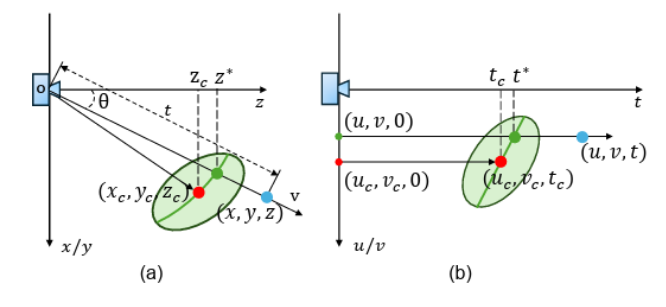
\includegraphics[width=1\linewidth]{../imagenes_marco_teorico/orden_profundidad_espacios.png}
    \caption{En (a), tenemos el espacio de la cámara. En (b), el espacio de rayos. La curva verde representa el conjunto de intersecciones con diferentes rayos de luz.}
    \label{espacio_rayos_camara}
\end{figure}

Notemos que los rayos de luz tienen vector director $(0,0,1)^T$ en el espacio de rayos.

Al transformar las gaussianas, tenemos funciones del tipo

\begin{equation}
G'(u) = e^{-(u-u_c)^T   \Sigma'^{-1}   (u-u_c)}
\end{equation}
con $u$ un punto en el espacio de rayos, $u_c$ y $\Sigma'$ la media y matriz de covarianzas transformadas, respectivamente. Notamos $u_c = (u_c, v_c, t_c)^T$. La matriz de covarianzas es la misma que calculamos anteriormente.

De forma análoga, el máximo se encuentra en

\begin{equation}
t^* = \frac{v'^T \Sigma'^{-1} (u_c - u_o)}{v'^T \Sigma'^{-1} v'}
\end{equation}

Pero, en este caso, la dirección $v'$ es el vector $(0,0,1)^T$, por lo que podemos precomputar $v'^T \Sigma'^{-1} v'$ y $v'^T \Sigma'^{-1}$ para cada gaussiana. Así, el punto de intersección lo podemos reescribir como

\begin{equation}
t^* = \hat{q}(u_c-u_o)
\end{equation}

Como podemos ver a partir de la figura \ref{espacio_rayos_camara}, $t$ es la distancia entre el punto tridimensional $x$ y el centro de la cámara $o$. Así que la profundidad de $x$ es
\begin{equation}
d = cos\theta \cdot t^*
\end{equation}

con $\theta$ el ángulo entre el rayo de luz y el eje principal de la cámara. Para simplificarlo, \cite{zhang2024radegs} aproxima por $\theta_c$, el ángulo definido por la media $x_c$ de la gaussiana. Así, la profundidad $x$ es
\begin{equation}
d = cos\theta_c \cdot t^* = \frac{z_c}{t_c} t^* = \frac{z_c}{t_c} \hat{q} (u_c - u_o)
= \hat{p}(u_c - u_o)
\end{equation}
tomando $\hat{p} = \frac{z_c}{t_c} \hat{q}$ constante para cada gaussiana.

Luego, podemos reformular la ecuación una vez más como
\begin{equation}
d = \hat{p}(u_c - u_o) = \hat{p}(u_c-u,v_c-v,t_c) = \hat{p}(0,0,t_c) + \hat{p}(u_c-u, v_c-v,0)
\end{equation}

El primer sumando, podemos simplificar:

\begin{equation}
\hat{p}(0,0,t_c) = \frac{z_c}{t_c}\hat{p}(0,0,t_c) = \frac{z_c}{t_c} \frac{v'^T \Sigma'^{-1}}{v'^T \Sigma'^{-1}v'} (0,0,t_c) = \frac{z_c}{t_c} \frac{v'^T \Sigma'^{-1}}{v'^T \Sigma'^{-1}v'} (t_c v')
= \frac{z_c}{t_c} \frac{v'^T \Sigma'^{-1} v'}{v'^T \Sigma'^{-1}v'} t_c = z_c
\end{equation}

En el segundo sumado, como el tercer elemento del vector derecho es 0, podemos saltear el tercer elemento de $\hat{p}$, obteniendo el $p$ que buscábamos.

Notemos que, en esta deducción, se introdujo un error al aproximar $\theta$ por $\theta_c$, pero este es despreciable debido a que la proyección local de una gaussiana es pequeña en una imagen dada. Así, los rayos tienen ángulos muy similares, por lo que no es necesario ajustar cuentas posteriores para tener en cuenta este error.

\subsection{Función de costo y gradientes}

Al tratarse de un problema de optimización, es necesario definir una función de costo que permita mejorar la calidad de la reconstrucción iterativamente. Esta función de costo varía en la literatura, pero comúnmente se compone del error fotométrico entre la imagen renderizada y la imagen observada, junto con términos de regularización que imponen restricciones sobre lo parámetros para controlar la estructura de la escena reconstruida.

Sea $\mathcal{L}$ la función de costo a minimizar, se calculan analíticamente los siguientes gradientes de $\mathcal{L}$ respecto de los parámetros de cada gaussiana:

\begin{itemize}
    \item \textbf{Gradiente de color:} Mide cómo ajustar el color de cada gaussiana para reducir la discrepancia entre la imagen renderizada y la observada.
    
    \item \textbf{Gradiente de opacidad:} Indica cómo modificar la transparencia de cada gaussiana para mejorar la correspondencia fotométrica.
    
    \item \textbf{Gradiente de media:} Permite ajustar la posición de cada gaussiana en el espacio tridimensional para mejorar la reconstrucción geométrica.
    
    \item \textbf{Gradiente de covarianza:} Informa sobre cómo modificar la forma y orientación de cada gaussiana para capturar mejor los detalles de la escena. Este se puede descomponer en gradientes de rotación y escala debido a la parametrización de la covarianza, permitiendo mantener la propiedad de semidefinida positiva durante la optimización y manteniendo su interpretación geométrica.


\end{itemize}

\subsection{Gestión de mapa}

Al renderizar imágenes a partir de los splats, existen zonas que podrían quedar subrepresentadas o sobrerepresentadas. Este problema está relacionado tanto con la posición como con la cantidad de gaussianas involucradas. Estas zonas tienen gradientes de posición elevados, lo cual se podría explicar con que la optimización trata de mover las gaussianas para corregir la reconstrucción local. Se identifican estos casos cuando el gradiente de posición supera un umbral, experimentalmente 0.0002.

Es posible mantener constantes las gaussianas y permitir que el algoritmo itere cuanto sea necesario, sin embargo, se obtienen mejores resultados empleando lo que se llama un control adaptativo:

\begin{itemize}
    \item Para las zonas subrepresentadas, tenemos gaussianas pequeñas que no logran representar la geometría local. La densificación, proceso por el cual se agregan gaussianas nuevas, se realiza clonando las gaussianas tales y moviendo la copia en el sentido del gradiente de posición. Al hacer esto, aumenta el volumen cubierto por las gaussianas, y la cantidad de las mismas.

    \item Para las zonas sobrerepresentadas, tenemos gaussianas con gran varianza, cubriendo áreas de elevado tamaño. En este caso, la densificación es a partir de la partición en dos gaussianas, dividiendo la escala por un factor $\phi = 1.6$ determinado experimentalmente. La posición de las dos resultantes se obtiene muestreando sobre la función de probabilidad de la gaussiana original. En este caso, el volumen cubierto por las gaussianas es el mismo, pero aumenta la cantidad.
\end{itemize}

\begin{figure}[H]
    \centering
    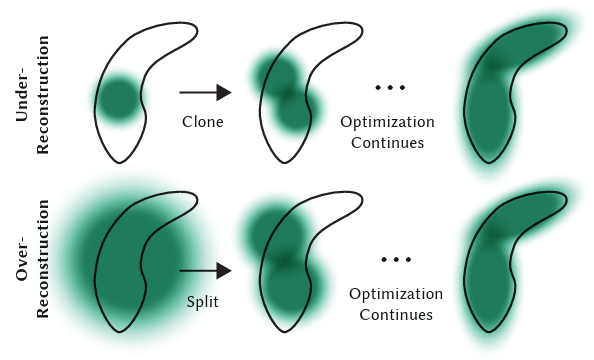
\includegraphics[width=0.75\linewidth]{../imagenes_marco_teorico/densificacion_gaussianas.png}
    \caption{Arriba, se observa la densificación en zonas subrepresentadas clonando la original. Abajo, tenemos la densificación en zonas sobrerepresentadas mediante la partición de la original. Imagen extraída de \cite{zhang2024radegs}}
\end{figure}

Por otro lado, la optimización de los parámetros podría dar lugar a gaussianas con $\alpha$ tan pequeño que su aporte en la representación sea fundamentalmente nulo. Debido a esto, otro paso para el control de gaussianas es la poda, eliminando aquellas con un $\alpha < \epsilon_\alpha$, siendo $\epsilon_\alpha$ un umbral.

Finalmente, el último criterio que se emplea para eliminar gaussianas es calcular la probabilidad de que se considere un \textit{outlier}, i.e., para cada píxel en el que participa durante la rasterización, si la gaussiana modela que el punto se encuentra arbitrariamente más cerca de lo medido, aumenta la probabilidad de ser \textit{outlier}. Experimentalmente, el criterio usa $<0.8d$ con $d$ la distancia medida. Luego, se obtiene la proporción de veces que fue \textit{outlier} para comparar con un umbral inferior, tal que si lo supera es removida.

En este trabajo se exploran distintas heurísticas para la gestión de mapa, las cuales afectarán la densificación de zonas subrepresentadas.






\section{Unidad de medición inercial}
Dependiendo del robot, es posible disponer de más tipos de sensores que aprovechar para tareas de SLAM. Tal es el caso de la Unidad de Medición Inercial (IMU). Su trabajo es medir la aceleración, rotación y velocidad de un objeto, en nuestro caso el robot. En SLAM, se emplean preintegrando sus mediciones para obtener estimaciones de la pose, esto es, sumando mediciones en un rango temporal de forma adecuada para estimar desplazamientos y rotaciones.

\begin{figure}[H]
    \centering
    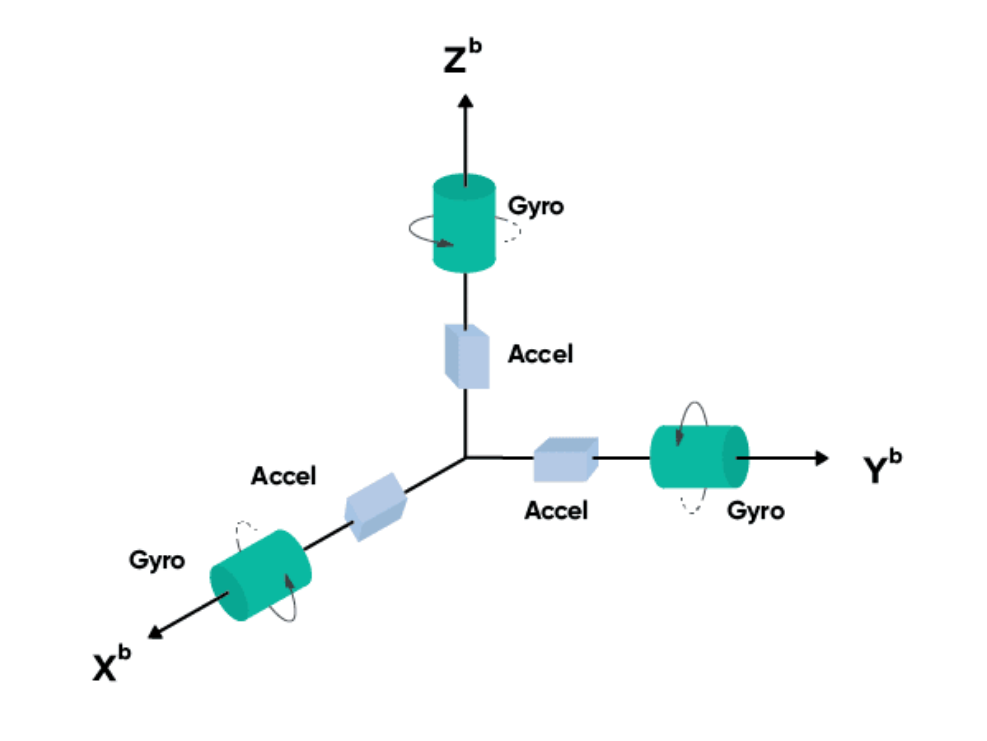
\includegraphics[width=0.5\linewidth]{../imagenes_marco_teorico/giroscopio_ejes.png}
    \caption{Se observa el tipo de dato obtenido de una IMU. Para cada eje, la aceleración y rotación correspondiente. Imagen extraída de \cite{advancednavigation_imu_intro}}
\end{figure}

Se clasifican en cuatro grados según su precisión \cite{10814674}: para consumo, de uso industrial, de uso táctico, y para navegación. Los de menor grado se basan en sistemas micro-electromecánicos que miden la aceleración lineal y angular según el movimiento de masas suspendidas. En este sistema hay dos componentes principales: el acelerómetro y el giróscopo. 

\begin{figure}[H]
    \centering
    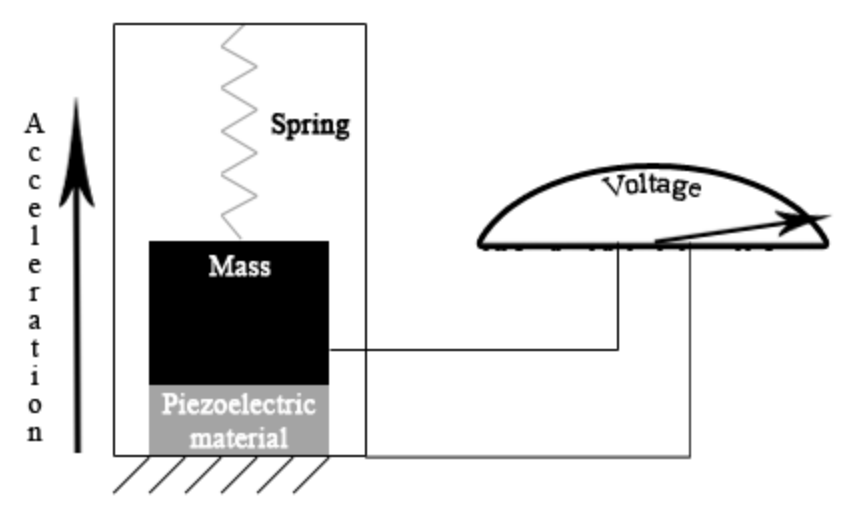
\includegraphics[width=0.8\linewidth]{../imagenes_marco_teorico/modelo_acelerometro_resorte.png}
    \caption{Modelo de acelerómetro para un eje particular. Imagen extraída de \cite{toniK_accelerometer_basics}.}
    \label{fig:acelerometro}
\end{figure}

En un acelerómetro, para cada eje hay una masa suspendida conectada a un resorte. Al percibir una aceleración en el eje correspondiente, en el caso de \ref{fig:acelerometro} hacia la parte superior de la imagen, por inercia la masa ejercerá presión sobre un material piezoeléctrico, el cual generará un voltaje proporcional a la presión recibida, el cual será traducido posteriormente a una medida de aceleración.

\begin{figure}[H]
    \centering
    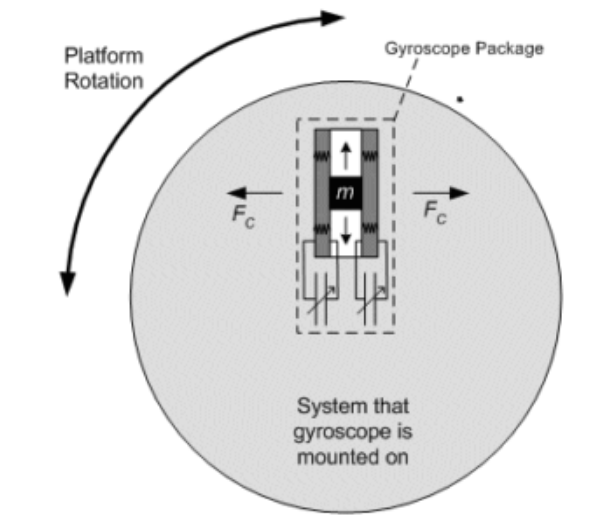
\includegraphics[width=0.5\linewidth]{../imagenes_marco_teorico/modelo_giroscopo.png}
    \caption{Modelo de un giróscopo en un eje particular. Imagen extraída de \cite{ericco2019memsgyro}.}
    \label{fig:giroscopio}
\end{figure}

En un giróscopo, una de las formas de medir la velocidad angular consiste en utilizar una masa suspendida para cada eje, a la cual se le induce una vibración continua. Debido al efecto Coriolis, cuando existe una rotación alrededor del eje correspondiente aparece una fuerza sobre la masa vibrante, perpendicular a su dirección de movimiento.

Esta fuerza provoca un pequeño desplazamiento lateral de la masa, lo que genera una diferencia de capacitancia entre electrodos ubicados a los lados del sensor. Dicha variación capacitiva se traduce en una señal eléctrica que puede utilizarse para estimar la velocidad angular del sistema.

En el caso de la Figura \ref{fig:giroscopio}, si hubiera una rotación en sentido horario y la masa estuviera vibrando de abajo hacia arriba, es decir, desde el centro hacia el borde, se produciría una fuerza lateral hacia la izquierda.



Los sistemas inerciales de menor grado son los más accesibles, pero sus sesgos crecen rápido, degenerando la integración de la pose en pocos segundos. Los de mayor grado poseen, además, giróscopos de fibra óptica, que miden el ratio angular enviando dos rayos de luz. Los mismos viajan en direcciones opuestas a través de un círculo de fibra óptica y vuelven a un sensor. De no haber rotación, volverían al mismo tiempo, y de haber, cambiaría el tiempo de alguno de los dos siguiendo el efecto Sagnac \cite{canalgeomatics_fiberopticgyros}.

\begin{table}[H]
\centering
\caption{Clasificación de IMUs según el sesgo del giróscopo y sus aplicaciones típicas.}
\label{tab:sesgos_imu}
\begin{tabular}{l c p{7cm}}
\toprule
\textbf{Grado} & \textbf{Sesgo del giróscopo (°/h)} & \textbf{Aplicaciones} \\
\midrule
Consumo      & $> 10$           & Teléfonos celulares, relojes inteligentes, controles de videojuegos \\
Industrial   & $1$ -- $10$       & Drones, robótica móvil, automoción \\
Táctico      & $0.1$ -- $1$      & UAVs, sistemas de defensa, instrumentación industrial de precisión \\
Navegación   & $< 0.01$          & Aeroespacial, submarinos, navegación inercial de alta precisión \\
\bottomrule
\end{tabular}
\end{table} 

\subsection{Cinemática de la IMU}

Para modelar el comportamiento de los sensores, se describe su cinemática en \cite{LeuteneggerLynenBosseSiegwartFurgale2015} del siguiente modo:

Sea $\mb{C}_{AB}$ la matriz de rotación de $B$ a $A$, $\mb{\rho}$ la posición, $\mb{q}$ la rotación, $\mb{v}$ la velocidad, ${}_ca_b$ el vector $a$ de $b$ expresado en el sistema de referencia $c$, $\mb{a}$ la aceleración, $\mb{b}_a, \mb{b}_g$ los sesgos del acelerómetro y giróscopo. Asumiendo que la rotación de la Tierra es despreciable respecto a las medidas del giroscopio, tenemos el modelo no lineal:

\begin{equation}
\begin{aligned}
{}_{w}\dot{\mathbf{\rho}}_{s} &= \mathbf{C}_{ws}\,{}_{s}\mathbf{v}, \\[4pt]
%
\dot{\mathbf{q}}_{ws} &= \frac{1}{2}\,\boldsymbol{\Omega}\!\left({}_{s}\boldsymbol{\omega}\right)\,\mathbf{q}_{ws}, \\[6pt]
%
{}_{s}\dot{\mathbf{v}} &=
{}_{s}\tilde{\mathbf{a}}
+ \mathbf{w}_{a}
- \mathbf{b}_{a}
+ \mathbf{C}_{sw}\,{}_{w}\mathbf{g}
- \left({}_{s}\boldsymbol{\omega}\right) \times {}_{s}\mathbf{v}, \\[6pt]
%
\dot{\mathbf{b}}_{g} &= \mathbf{w}_{b_g}, \\[4pt]
%
\dot{\mathbf{b}}_{a} &= -\frac{1}{\tau}\,\mathbf{b}_{a} + \mathbf{w}_{b_a}.
\label{imu_formula}
\end{aligned}
\end{equation}


con $\mathbf{w}_i$ ruidos gaussianos de media cero y la matriz $\Omega$ formada por el ratio angular estimado ${}_s\omega = {}_s\tilde{\omega} + \mathbf{w}_g - \mathbf{b}_g$ a partir de la medida ${}_s\tilde{\omega}$. En esta formulación, la actualización del cuaternión se interpreta como una perturbación a izquierda:

\[
\Omega({}_s\omega)\,\mathbf{q}_{ws} = \mathbf{q}_{ws} \oplus_{\mathrm{izq}} {}_s\boldsymbol{\omega}.
\]

Se usa esta convención porque la cinemática está escrita en el marco del sensor y el término incremental se aplica por pre-multiplicación.

La primera ecuación describe la evolución de la posición del sensor $s$ en coordenadas globales $w$, dada por la velocidad expresada en el marco del sensor multiplicada por un cambio de base que lleva su rotación al marco global.

La segunda ecuación describe la evolución de la rotación, expresada en cuaterniones, como la suma en el grupo $SO(3)$ de la rotación y la estimación del ratio angular medido.

La tercera ecuación describe la evolución de la velocidad, es decir la aceleración, en el marco del sensor. Comienza con la aceleración medida, a la cual se le suma un ruido gaussiano del acelerómetro. Este ruido surge inherentemente al modelar sensores. Por otro lado, se le resta el sesgo del acelerómetro y se le suma la gravedad rotada a las coordenadas del sensor. Finalmente, se le resta el producto cruz entre el ratio angular estimado del sensor y su velocidad, como corrección del efecto Coriolis.

La cuarta ecuación describe la evolución del sesgo del giroscopio como un ruido gaussiano de media cero, mientras que la quinta ecuación describe la evolución del sesgo del acelerómetro como un ruido gaussiano también, aunque compensado por una fuerza que tiende a mantenerlo alrededor del cero a partir de una constante temporal $\tau > 0$.

Notemos que, al modelar ambos ruidos con variables aleatorias, nos encontramos con lo que se conoce como camino aleatorio y camino aleatorio acotado, respectivamente. Este comportamiento los hace difíciles de controlar, y provoca que un sistema de estimación de la pose basado exclusivamente en las mediciones inerciales tienda a degenerarse a medida que pasa el tiempo. Para contrarrestar este fenómeno, se hace lo siguiente:

Al iniciar el robot, se lo deja quieto unos segundos. Luego, se toma el promedio de las mediciones de aceleración y rotación, y se las considera el sesgo a restar. Esta estimación permite una inicialización razonable del sistema, pero la evolución temporal la hará inestable. Para contrarrestarlo, es necesario correlacionar los datos con los de otros sensores. Históricamente, los filtros de Kalman \cite{MasnadiShirazi2019KalmanTutorial} constituyen una técnica muy empleada para fusionar los distintos sensores a partir de matrices, pero en el marco de este trabajo no es factible. Esto se debe a que el modelo que empleamos es no lineal, se basa en algoritmos iterativos de optimización con derivadas, y que el gran número de gaussianas da lugar a demasiados parámetros a optimizar. De este modo, el sesgo se corrige mediante algoritmos de optimización que fusionan los datos visuales con los inerciales.

%\section{VIGS-Fusion}
El paper que inspiró este trabajo, llamado VIGS-Fusion \cite{ndoye2025vigs}, realizó una versión de Gaussian Splatting para reconstrucción tridimensional a partir de datos de una cámara RGB-D y una IMU. El trabajo fue preparado para ser implementado en un UAV pequeño a tiempo real, por lo que era fundamental una eficiencia temporal elevada y resultados robustos. 
A partir de plantear un problema de optimización que incluye los sesgos de la IMU, logró velocidades de reconstrucción de hasta 30x las del estado del arte para SLAM con estos sensores. La modificación principal frente a los demás métodos de la literatura es que presentó tanto un marco de corrección para los sesgos de la IMU, como distintos cálculos para los gradientes de las gaussianas.

\begin{figure}[H]
    \centering
    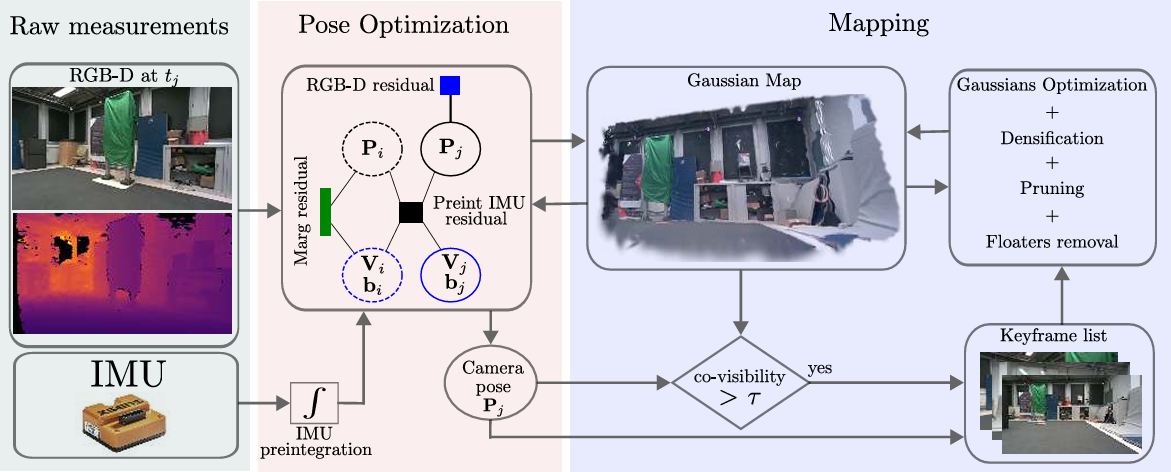
\includegraphics[width=0.75\linewidth]{../imagenes_marco_teorico/pipeline_vigs_fusion.png}
    \caption{Pipeline del paper VIGS-Fusion. Los keyframes son elegidos cuando la co-visibilidad con el frame actual supera un umbral $\tau$. En la optimización de la pose obtienen residuos de marginalización, de RGB-D y de la IMU.}
    \label{fig:pipeline_vigs_fusion}
\end{figure}

Ahora, veamos el método presentado por el paper.

\subsection{Optimización de la pose}

El estado a tiempo $k$ se define como

\begin{equation}
    x_k = [\mb{P}_k, \mb{V}_k, \mb{b}_a^k, \mb{b}_g^k]
\end{equation}

con $\mb{P}_k \in SE(3)$ representando la traslación $\mb{p}_k \in \mathbb{R}^3$ y la rotación $\mb{R}_k \in SO(3)$; $\mb{V}_k$ la velocidad; $\mb{b}_a^k$ y $\mb{b}_g^k$ los sesgos del acelerómetro y giróscopo, respectivamente.

Para optimizar, se define una función de costo general que combina los residuos de RGB-D, de IMU y de marginalización:

\begin{equation}
C(\mb{x}_k) = r_{RGB-D} + r_{IMU} + r_{Marg}
\end{equation}

Para la minimización se utilizó Levenberg-Marquadt, con una aproximación del segundo orden $r_{RGB-D}$, en contraste con los métodos del estado del arte que utilizaban descenso del gradiente de primer orden.

Para calcular el Jacobiano respecto de la pose $\mb{P}_k$, se planteó desde el álgebra de Lie, teniendo en cuenta que $\mb{P}_k \in SE(3)$ induce una representación $\xi_k = [\rho, \omega]^T \in \mathfrak{se}(3)$ con $\rho \in \mathbb{R}^3$ la traslación y $\omega \in \mathbb{R}^3$ la rotación. En este caso, la actualización se hace con perturbación a izquierda, porque el paper premultiplica el incremento al estado:

\begin{equation}
\mb{P}_{k+1} = \exp(\delta \xi)\,\mb{P}_k = \delta \xi \oplus_{\mathrm{izq}} \mb{P}_k
\end{equation}

Esta convención se conserva aquí para mantener la formulación original del método, pero queda explícito que la perturbación es a izquierda.

\subsection{Residuo RGB-D}
Este residuo se compone del residuo fotométrico, que es la diferencia entre el color observado y el renderizado, $r_{photo} = RGB(x) - C(x)$, y el residuo geométrico, que es la diferencia entre la profundidad observada y la renderizada, $r_{geo} = D(x) - d(x)$. Para calcular la profundidad renderizada $d(x)$ se consideró la mediana de las profundidades de las gaussianas calculadas con \ref{profundidad_gaussianas}.

\begin{equation}
r_{RGB-D} = r_{photo} + r_{geo}
\end{equation}

En la literatura, se utiliza descenso del gradiente computando el Jacobiano a partir del modelo de color y profundidad, requiriendo muchos parámetros para poder diferenciar la suma de gaussianas pesadas. En este paper, se determinó un cambio que consiste en usar las derivadas de la imagen observada en el espacio bidimensional. Para obtener los Jacobianos se diferenciaron el color observado $RGB(x)$ y la profundidad $D(x)$.

\subsubsection{Jacobiano del error fotométrico}

\begin{equation}
\mb{J}_{\xi_c}^{r_{photo}} = \frac{\mc{D}r_{photo}}{\mc{D}\xi_c} = 
\frac{\mc{D}(RGB(x) - C(x))}{\mc{D}\xi_c} = \frac{\mc{D}RGB(x)}{\mc{D}\xi_c}
\label{jacobiano_error_fotometrico}
\end{equation}

Utilizando los gradientes de la imagen observada, se aplicó la regla de la cadena

\begin{equation}
\frac{\mc{D}RGB(x)}{\mc{D}\xi_c} = \frac{\mc{D}RGB(x)}{\mc{D}\mb{u}} 
\frac{\mc{D}\mb{u}}{\mc{D}\mb{u}_c} \frac{\mc{D}\mb{u}_c}{\mc{D}\xi_c}
\end{equation}

donde $\mb{u}(u_x, u_y)$ es la ubicación del píxel en el plano bidimensional, y $\mb{u}_c$ su ubicación en el espacio tridimensional en el sistema de referencia de la cámara.

A partir de esta descomposición, se tienen los siguientes términos:

\begin{itemize}
    \item 
    El gradiente de la imagen respecto de cada color y dirección:
    \begin{equation}
    \frac{\mc{D}RGB(x)}{\mc{D}\mb{u}} =
    \begin{bmatrix}
        g_{u_x}^R & g_{u_x}^G & g_{u_x}^B\\
        g_{u_y}^R & g_{u_y}^G & g_{u_y}^B
    \end{bmatrix} ^T
    \end{equation}
    donde $g_{u_a}^b$ representa el gradiente en la dirección $a$ del canal $b$.
    
    \item 
    El Jacobiano de la proyección de la cámara deducido en \ref{jacobiano_proyeccion_camara}.
    $\frac{\mc{D}\mb{u}}{\mc{D}\mb{u}_c} = \mb{J}_c$

    \item 
    El Jacobiano de los puntos respecto de un movimiento en la pose
    \begin{equation}
    \frac{\mc{D}\mb{u}_c}{\mc{D}\xi_c}
    \end{equation}
    Para encontrar una fórmula cerrada, \cite{Matsuki2024GaussianSplattingSLAM} utilizó la derivación en la variante. Así, la perturbación $\delta \xi_c$, descompuesta en su traslación $\rho'$ y su rotación $\omega'$ induce la acción sobre el punto
    
    \begin{equation}
    \mb{u}_c' = (\mb{I} + [\omega']_X) \mb{u}_c + \rho
    \end{equation}

    por lo que la perturbación lleva a la diferencia

    \begin{equation}
    \delta\mu_c = \mu_c' - \mu_c = \rho + [\omega]_X \mu_c = \rho - [\mu_c]_X \,\,\omega
    \end{equation}

    Luego, podemos expresar el Jacobiano como

    \begin{equation}
    \frac{\mc{D}\mb{u}_c}{\mc{D}\xi_c} = 
    \begin{bmatrix}
        \mb{I} & -[\mb{u}_c]_X
    \end{bmatrix}
    \label{jacobiano_puntos_pose}
    \end{equation}
\end{itemize}

\subsubsection{Jacobiano del error geométrico}

\begin{equation}
    \mb{J}_{\xi_c}^{r_{geo}} = \frac{\mc{D}(D(x) - d(x))}{\mc{D}\xi_c} = \frac{\mc{D}D(x)}{\mc{D}\xi_c}
\end{equation}

Mediante la regla de la cadena,

\begin{equation}
    \frac{\mc{D}D(x)}{\mc{D}\xi_c} = \frac{\mc{D}D(\mb{x})}{\mc{D}\mb{u}_c}
    \frac{\mc{D}\mb{u}_c}{\mc{D}\xi_c}
\end{equation}

De nuevo, tenemos una descomposición con los términos:

\begin{itemize}
    \item 
    La dirección del rayo. Despejando en \ref{proyeccion_pinhole}, surge que
    \begin{equation}
    \frac{\mc{D}D(\mb{x})}{\mc{D}\mb{u}_c} = r = 
    \begin{bmatrix}
        \frac{u_x - c_x}{f_x} \\
        \frac{u_y - c_y}{f_y}
    \end{bmatrix}
    \end{equation}

    \item 
    El Jacobiano de los puntos respecto de un movimiento en la pose, que ya calculamos en \ref{jacobiano_puntos_pose}
\end{itemize}



\subsubsection{Resultados para $r_{RGB-D}$}

Al plantear los residuos como una matriz de la forma

\begin{equation}
    \mb{r}_{RGB-D} =
    \begin{bmatrix}
        \mb{r}_{photo} \\
        \mb{r}_{geo}
    \end{bmatrix}
\end{equation}

se expresa el Jacobiano completo

\begin{equation}
    \mb{J}_{\xi_c}^{r_{RGB-D}} =
    \begin{bmatrix}
        \mb{J}_{\xi_c}^{r_{photo}} \\
        \mb{J}_{\xi_c}^{r_{geo}}
    \end{bmatrix}
\end{equation}

Luego, para poder usar Levenberg-Marquadt se tienen las expresiones

\begin{equation}
    {\mb{J}_{\xi_c}^{r_{RGB-D}}}^T \mb{J}_{\xi_c}^{r_{RGB-D}} =
    {\mb{J}_{\xi_c}^{r_{photo}}}^T \mb{J}_{\xi_c}^{r_{photo}} +
    {\mb{J}_{\xi_c}^{r_{geo}}}^T \mb{J}_{\xi_c}^{r_{geo}}
\end{equation}
    
\begin{equation}
    {\mb{J}_{\xi_c}^{r_{RGB-D}}}^T \mb{r}_{RGB-D} =
    {\mb{J}_{\xi_c}^{r_{photo}}}^T \mb{r}_{photo} +
    {\mb{J}_{\xi_c}^{r_{geo}}}^T \mb{r}_{geo}
\end{equation}


%%%%%%%%%%%%%%%%%%%%%%%%%

\subsection{Residuo IMU}

El estado del sistema en el instante $k$ se define como

\begin{equation}
\mathbf{x}_k =
\left(
\mathbf{p}_k,
\mathbf{q}_k,
\mathbf{v}_k,
\mathbf{b}_{a_k},
\mathbf{b}_{g_k}
\right)
\end{equation}

donde $\mathbf{p}_k$ es la posición, $\mathbf{q}_k$ la orientación, $\mathbf{v}_k$ la velocidad y $\mathbf{b}_{a_k},\mathbf{b}_{g_k}$ representan los sesgos del acelerómetro y el giroscopio respectivamente.

Entre dos fotogramas consecutivos $i$ y $j$, las mediciones de la IMU se preintegran obteniendo las cantidades

\begin{equation}
(\Delta \mathbf{p}_{ij}, \Delta \mathbf{v}_{ij}, \Delta \mathbf{q}_{ij})
\end{equation}

que representan los cambios relativos de posición, velocidad y orientación expresados en el sistema de referencia del instante $i$.

Siguiendo la formulación de la preintegración en variedades, la predicción del estado en el instante $j$ a partir del estado en $i$ puede escribirse como

\begin{align}
\mathbf{p}_j &=
\mathbf{p}_i
+
\mathbf{v}_i \Delta t
+
\frac12 \mathbf{g} \Delta t^2
+
\mathbf{R}_i
\Delta \mathbf{p}_{ij}
\\
\mathbf{v}_j &=
\mathbf{v}_i
+
\mathbf{g}\Delta t
+
\mathbf{R}_i
\Delta \mathbf{v}_{ij}
\\
\mathbf{q}_j &=
\mathbf{q}_i
\otimes
\Delta \mathbf{q}_{ij}
\end{align}

donde $\mathbf{R}_i$ es la matriz de rotación asociada al cuaternión $\mathbf{q}_i$.

El residuo IMU compara la predicción obtenida mediante estas ecuaciones con el estado estimado por el optimizador. Se define entonces como

\begin{equation}
\mathbf{r}_{IMU}
=
\begin{bmatrix}
\mathbf{r}_p \\
\mathbf{r}_q \\
\mathbf{r}_v \\
\mathbf{r}_{ba} \\
\mathbf{r}_{bg}
\end{bmatrix}
\end{equation}

donde cada componente corresponde a un error en posición, orientación, velocidad y sesgos.

El residuo de posición se define como

\begin{equation}
\mathbf{r}_p =
\mathbf{R}_i^\top
\left(
\mathbf{p}_j
-
\mathbf{p}_i
-
\mathbf{v}_i \Delta t
-
\frac12 \mathbf{g}\Delta t^2
\right)
-
\Delta \mathbf{p}_{ij}
\end{equation}

El residuo de velocidad se expresa como

\begin{equation}
\mathbf{r}_v =
\mathbf{R}_i^\top
\left(
\mathbf{v}_j
-
\mathbf{v}_i
-
\mathbf{g}\Delta t
\right)
-
\Delta \mathbf{v}_{ij}
\end{equation}

Para la orientación se utiliza la diferencia de cuaterniones en el grupo $SO(3)$

\begin{equation}
\mathbf{r}_q =
(\mathbf{q}_i^{-1}\mathbf{q}_j)
\ominus
\Delta\mathbf{q}_{ij}
\end{equation}

Utilizando la parametrización mínima del error rotacional en $SO(3)$, este término puede escribirse explícitamente como

\begin{equation}
\mathbf{r}_q =
2\,\mathrm{vec}
\left(
\Delta \mathbf{q}_{ij}^{-1}
(\mathbf{q}_i^{-1}\mathbf{q}_j)
\right).
\end{equation}

donde $\mathrm{vec}(\cdot)$ extrae la parte vectorial del cuaternión.

Los residuos asociados a los sesgos se definen como

\begin{align}
\mathbf{r}_{ba} &= \mathbf{b}_{a_j} - \mathbf{b}_{a_i} \\
\mathbf{r}_{bg} &= \mathbf{b}_{g_j} - \mathbf{b}_{g_i}
\end{align}

Para resolver el problema mediante optimización no lineal, el residuo se linealiza alrededor de una estimación actual $\tilde{\mathbf{x}}$.

\begin{equation}
\mathbf{r}_{IMU}(\mathbf{x})
\approx
\mathbf{r}_{IMU}(\tilde{\mathbf{x}})
+
\mathbf{J}
\delta \mathbf{x}
\end{equation}

donde

\begin{equation}
\mathbf{J}
=
\frac{\partial \mathbf{r}_{IMU}}{\partial \mathbf{x}}
\end{equation}

es el Jacobiano del residuo respecto al estado.

Por ejemplo, derivando el residuo de posición respecto a $\mathbf{p}_i$ se obtiene

\begin{equation}
\frac{\partial \mathbf{r}_p}{\partial \mathbf{p}_i}
=
-\mathbf{R}_i^\top
\end{equation}

mientras que respecto a $\mathbf{p}_j$

\begin{equation}
\frac{\partial \mathbf{r}_p}{\partial \mathbf{p}_j}
=
\mathbf{R}_i^\top
\end{equation}

y respecto a la velocidad inicial

\begin{equation}
\frac{\partial \mathbf{r}_p}{\partial \mathbf{v}_i}
=
-\mathbf{R}_i^\top \Delta t
\end{equation}

Las derivadas respecto a la orientación utilizan la aproximación de primer orden de la rotación

\begin{equation}
\mathbf{R}(\delta \boldsymbol{\theta})
\approx
\mathbf{I}
+
[\delta \boldsymbol{\theta}]_\times
\end{equation}

Finalmente, los residuos se ponderan mediante la matriz de información de la medición

\begin{equation}
\|r\|^2 =
\mathbf{r}_{IMU}^\top
\mathbf{W}
\mathbf{r}_{IMU}
\end{equation}

donde $\mathbf{W}=\boldsymbol{\Sigma}^{-1}$ es la inversa de la covarianza de la preintegración.



%%%%%%%%%%%%%%%%%%%%%%%%%%%%%%%%%%%%%%%%%%%%%%%
\subsection{Residuo de marginalización}

Al obtener nuevos datos, el sistema estima un nuevo estado $\mathbf{x}_k$. 
Para mantener el problema de optimización computacionalmente manejable, se utiliza 
una estrategia de \textit{ventana deslizante}, donde los estados más antiguos se eliminan 
de la optimización. Sin embargo, eliminar directamente dichos estados implicaría perder 
la información contenida en las mediciones asociadas a ellos. 

Para evitar esta pérdida de información, se realiza un proceso de \textit{marginalización}, 
mediante el cual las variables antiguas se eliminan del problema pero su información se 
condensa en un nuevo factor que actúa como un prior sobre las variables restantes.

Sea el vector completo de variables del problema

\begin{equation}
\mathbf{x} =
\begin{bmatrix}
\mathbf{x}_m \\
\mathbf{x}_r
\end{bmatrix}
\end{equation}

donde

\begin{itemize}
\item $\mathbf{x}_m$ representa las variables que se desean marginalizar (estados antiguos),
\item $\mathbf{x}_r$ representa las variables que permanecerán en la optimización.
\end{itemize}

El problema de mínimos cuadrados puede escribirse como

\begin{equation}
\min_{\mathbf{x}}
\|\mathbf{r}(\mathbf{x})\|^2
\end{equation}

donde $\mathbf{r}(\mathbf{x})$ es el vector de residuos del sistema.

Linealizando alrededor de una estimación actual $\tilde{\mathbf{x}}$ se obtiene

\begin{equation}
\mathbf{r}(\mathbf{x})
\approx
\mathbf{r}_0 + \mathbf{J}\delta\mathbf{x}
\end{equation}

donde

\begin{equation}
\delta\mathbf{x} =
\mathbf{x} \ominus \tilde{\mathbf{x}}
\end{equation}

y $\mathbf{J}$ es el Jacobiano del residuo.

El sistema normal asociado al problema de mínimos cuadrados es

\begin{equation}
\mathbf{A}\delta\mathbf{x} = \mathbf{b}
\end{equation}

con

\begin{align}
\mathbf{A} &= \mathbf{J}^\top \mathbf{J} \\
\mathbf{b} &= \mathbf{J}^\top \mathbf{r}_0
\end{align}

Separando las variables a marginalizar y las variables restantes, la matriz 
$\mathbf{A}$ puede escribirse como

\begin{equation}
\mathbf{A} =
\begin{bmatrix}
\mathbf{A}_{mm} & \mathbf{A}_{mr} \\
\mathbf{A}_{rm} & \mathbf{A}_{rr}
\end{bmatrix}
\end{equation}

y el vector $\mathbf{b}$ como

\begin{equation}
\mathbf{b} =
\begin{bmatrix}
\mathbf{b}_m \\
\mathbf{b}_r
\end{bmatrix}.
\end{equation}

Para eliminar las variables $\mathbf{x}_m$ se aplica el complemento de Schur, 
obteniéndose un nuevo sistema reducido

\begin{align}
\mathbf{A}^\ast &= 
\mathbf{A}_{rr} -
\mathbf{A}_{rm}
\mathbf{A}_{mm}^{-1}
\mathbf{A}_{mr}
\\
\mathbf{b}^\ast &=
\mathbf{b}_r -
\mathbf{A}_{rm}
\mathbf{A}_{mm}^{-1}
\mathbf{b}_m
\end{align}

que depende únicamente de las variables restantes $\mathbf{x}_r$.

Este sistema reducido define un nuevo factor que encapsula la información de las 
variables marginalizadas.

Para integrarlo nuevamente en el optimizador, se busca una factorización de la forma

\begin{equation}
\mathbf{A}^\ast =
\mathbf{J}_{marg}^\top
\mathbf{J}_{marg}
\end{equation}

donde $\mathbf{J}_{marg}$ es el jacobiano del nuevo factor de marginalización.

En la implementación, esta factorización se obtiene mediante descomposición espectral

\begin{equation}
\mathbf{A}^\ast =
\mathbf{V}
\mathbf{\Lambda}
\mathbf{V}^\top
\end{equation}

de donde se define

\begin{equation}
\mathbf{J}_{marg} =
\sqrt{\mathbf{\Lambda}}
\mathbf{V}^\top .
\end{equation}

El residuo asociado al factor de marginalización se define entonces como

\begin{equation}
\mathbf{r}_{marg}(\mathbf{x}_r)
=
\mathbf{r}_0
+
\mathbf{J}_{marg}
\delta\mathbf{x}_r
\end{equation}

donde

\begin{equation}
\mathbf{r}_0 =
\mathbf{J}_{marg}^{-T}
\mathbf{b}^\ast .
\end{equation}

Finalmente, el incremento de estado utilizado en la evaluación del residuo es

\begin{equation}
\delta\mathbf{x}_r =
\mathbf{x}_r \ominus \mathbf{x}_r^0
\end{equation}

donde $\mathbf{x}_r^0$ es el punto de linearización almacenado en el momento de 
realizar la marginalización.

En el caso de variables definidas en $SE(3)$, el incremento se calcula en el 
espacio tangente. Para una pose representada por posición $\mathbf{p}$ y 
cuaternión $\mathbf{q}$ se utiliza

\begin{equation}
\delta\mathbf{x} =
\begin{bmatrix}
\mathbf{p}-\mathbf{p}_0 \\
2\,\mathrm{vec}
\left(
\mathbf{q}_0^{-1}\mathbf{q}
\right)
\end{bmatrix}.
\end{equation}

De esta manera, el factor de marginalización actúa como un prior gaussiano 
sobre las variables restantes, preservando la información de los estados 
eliminados mientras se mantiene constante el tamaño del problema de optimización.




%%%%%%%%%%%%%%%%%%%%%%%%%%%%%%%%%%%%%%%%%%%%%%%%%%%%%%%%%%%%%%%%%%%%%%%%%%%%%%%%

\subsection{Función de costo para gaussianas}

En este trabajo se utiliza una función de costo compuesta por tres términos, análoga a la de otros trabajos como RAD-GS \cite{radgs}:

\begin{equation}
\mathcal{L} = \mathcal{L}_{\text{rgb}} + w_{\text{depth}} \mathcal{L}_{\text{depth}} + w_{\text{dist}} \mathcal{L}_{\text{dist}} + \lambda_{\text{iso}} \mathcal{L}_{\text{iso}}
\end{equation}

donde:

\paragraph{Término fotométrico ($\mathcal{L}_{\text{rgb}}$):}
Mide la diferencia cuadrática entre el color renderizado y el observado en cada píxel:
\begin{equation}
\mathcal{L}_{\text{rgb}} = \sum_{p} \frac{1}{2}\|C(p) - C^*(p)\|_2^2
\end{equation}
con $C(p) = \sum_n T_n \alpha_n c_n$ el color renderizado mediante alpha-blending ordenado en profundidad.

\paragraph{Término de profundidad mediana ($\mathcal{L}_{\text{depth}}$):}
Penaliza la diferencia entre la profundidad renderizada en el punto mediano de transmitancia (cuando $T$ cruza 0.5) y la profundidad observada:
\begin{equation}
\mathcal{L}_{\text{depth}} = \sum_{p} \frac{w_{\text{depth}}}{2}\, \mathbf{1}_{\text{med}}(p)\, \big(D_{\text{med}}(p) - D^*(p)\big)^2
\end{equation}
donde $\mathbf{1}_{\text{med}}(p)$ es un indicador que vale 1 en el splat donde la transmitancia cruza 0.5, y la profundidad en ese punto es:
\begin{equation}
D_{\text{med}}(p) = z_n + \hat{p}_n \cdot (p - \mu_n^{2D})
\end{equation}
con $\hat{p}_n$ el vector que codifica cómo varía la profundidad con el desplazamiento en imagen.

\paragraph{Término de distorsión de profundidad ($\mathcal{L}_{\text{dist}}$):}
Regulariza la consistencia entre la profundidad de cada splat y la profundidad mediana acumulada, pesando por la contribución de cada gaussiana:
\begin{equation}
\mathcal{L}_{\text{dist}} = \sum_{p,n} \frac{w_{\text{dist}}}{2}\, \alpha_n(p)\,T_n(p)\, \big(d_n(p)-D_{\text{med}}(p)\big)^2
\end{equation}
donde $d_n(p) = z_n + \hat{p}_n \cdot (p - \mu_n^{2D})$ es la profundidad de la gaussiana $n$ en el píxel $p$.

\paragraph{Término de regularización isotrópica ($\mathcal{L}_{\text{iso}}$):}

Penaliza que las gaussianas sean muy anisótropas (muy alargadas en una dirección), favoreciendo formas más esféricas:

\begin{equation}
\mathcal{L}_{\text{iso}} = \sum_{n} \lambda_{\text{iso}}\sum_{i} (s_{n,i} - \bar{s}_n)^2
\end{equation}
donde $s_{n,i}$ son las componentes de escala de la gaussiana $n$ y $\bar{s}_n = (s_{n,x} + s_{n,y} + s_{n,z})/3$.

Esta formulación permite balancear la fidelidad fotométrica con restricciones geométricas provenientes de sensores RGB-D, crucial para mantener una reconstrucción métrica consistente en SLAM visual.




\subsection{Gradientes}

Dada la función de costo, ahora podemos calcular los gradientes respecto de los parámetros de las gaussianas. Para esto, VIGS-Fusion plantea cálculo sobre las imágenes proyectadas, simplificando el costo computacional de las derivadas. A continuación, se detallan los cálculos para cada tipo de parámetro.

\subsubsection{Gradiente de color}

El color se forma a partir del alpha-blending de los splats bidimensionales. Por tanto,

\begin{equation}
C = \sum_n T_n \alpha_n c_n
\end{equation}

con $T_n$ la transmitancia, $\alpha_n$ la opacidad y $c_n$ el color de la gaussiana $n$ en orden de profundidad back-to-front.

Luego, tenemos que, sea $e = C - C_{obs}$ tal que $L = \frac{1}{2}||e||^2$ sea la función de pérdida,

\begin{equation}
    \frac{\partial L}{\partial c_n} = 
    \frac{\partial L}{\partial C} \frac{\partial C}{\partial c_n} =
    e (T_n\alpha_n)
\end{equation}

Ahora, para poder extenderlo a la gaussiana tridimensional, no es necesario realizar ningún cambio, ya que el color no se perturba al proyectar. Podemos simplemente usar

\begin{equation}
    \frac{\partial L}{\partial c_n^{3d}} = \frac{\partial L}{\partial c_n^{2d}}
\end{equation}



\subsubsection{Gradiente de opacidad}

Para la opacidad $\alpha_n$, tenemos que la misma influye activamente en el término correspondiente a la gaussiana $n$, y en todas las posteriores a partir del alpha-blending, pues

\begin{equation}
T_n = \prod_{k<n}(1-\alpha_k) 
\end{equation}

Al derivar, tenemos tanto el término propio de color $T_n \alpha_n c_n$ como todos los términos posteriores. Como el término propio es lineal en $\alpha_n$, la derivada es simplemente $T_n c_n$. Por otro lado, para un $m>n$ fijo,

\begin{equation}
\frac{\partial T_m}{\partial \alpha_n} = - \frac{T_m}{1 - \alpha_n}
\end{equation}

Luego,

\begin{equation}
    \frac{\partial C}{\partial \alpha_n} = T_nc_n - \frac{1}{1-\alpha_n} \sum_{m>n}T_m\alpha_mc_m
    = T_n c_n - \frac{C - C_{\leq n}}{1-\alpha_n}
\end{equation}

con $C_{\leq n}$ el color acumulado hasta n.

Finalmente,

\begin{equation}
    \frac{\partial L}{\partial \alpha_n} = 
    \frac{\partial L}{\partial C} \frac{\partial C}{\partial \alpha_n} =
    e (T_n c_n - \frac{C - C_{\leq n}}{1-\alpha_n})
\end{equation}


\subsubsection{Gradiente de la media}

Para calcular el gradiente de la media $\mu_{3D}$, lo separamos en:

\begin{equation}
    \frac{\partial L}{\partial \mu_{3D}} =
    \frac{\partial L}{\partial \mu_{2D}} \frac{\partial \mu_{2D}}{\partial \mu_{3D}}
    + \frac{\partial L}{\partial z} \frac{\partial z}{\partial \mu_{3D}}
    + \frac{\partial L}{\partial \Sigma'} \frac{\partial \Sigma'}{\partial \mu_{3D}}
\end{equation}

Ahora, deducimos cada término

\paragraph{Media bidimensional}

Sea $\mb{J}$ el jacobiano de la proyección,

\begin{equation}
    \frac{\partial \mu_{2D}}{\partial \mu_{3D}} = \mb{J}
\end{equation}

Para el factor restante, observamos que la media bidimensional influye en la
pérdida a través del peso gaussiano proyectado. Sea

\begin{equation}
G(x) =
\exp\!\left(
-\frac{1}{2} (x-\mu_{2D})^T \Sigma'^{-1} (x-\mu_{2D})
\right),
\end{equation}

y sea $\alpha = \sigma G$ la opacidad efectiva del splat en el píxel.
Entonces,

\begin{equation}
\frac{\partial \alpha}{\partial \mu_{2D}}
=
\alpha \, \Sigma'^{-1}(x-\mu_{2D}).
\end{equation}

Aplicando regla de la cadena,

\begin{equation}
\frac{\partial L}{\partial \mu_{2D}}
=
\frac{\partial L}{\partial \alpha}
\frac{\partial \alpha}{\partial \mu_{2D}}
=
\frac{\partial L}{\partial \alpha}
\alpha
\Sigma'^{-1}(x-\mu_{2D}).
\end{equation}

\paragraph{Profundidad}

La coordenada de profundidad es simplemente la tercera componente de la media en el sistema de referencia de la cámara:

\begin{equation}
    z = \mu_{3D,z}
\end{equation}

Por lo tanto,

\begin{equation}
    \frac{\partial z}{\partial \mu_{3D}} =
    \begin{bmatrix}
        0 & 0 & 1
    \end{bmatrix}
\end{equation}

y el término correspondiente del gradiente queda

\begin{equation}
    \frac{\partial L}{\partial z}
    \frac{\partial z}{\partial \mu_{3D}}
    =
    \frac{\partial L}{\partial z}
    \begin{bmatrix}
        0 & 0 & 1
    \end{bmatrix}.
\end{equation}

Para obtener $\frac{\partial \mathcal{L}}{\partial z}$, observamos que la profundidad aparece en dos lugares de la función de costo:

\paragraph{Deducción del gradiente del término de profundidad mediana}

El término de profundidad mediana es:
\begin{equation}
\mathcal{L}_{\text{depth}} = \sum_{p} \frac{w_{\text{depth}}}{2}\, \mathbf{1}_{\text{med}}(p)\, \big(D_{\text{med}}(p) - D^*(p)\big)^2
\end{equation}

Recordando que $D_{\text{med}}(p) = z_n + \hat{p}_n \cdot (p - \mu_n^{2D})$ para la gaussiana $n$ donde $T$ cruza 0.5, derivamos respecto a $z_n$:

\begin{equation}
\begin{split}
\frac{\partial \mathcal{L}_{\text{depth}}}{\partial z_n} &= \sum_{p} w_{\text{depth}} \, \mathbf{1}_{\text{med}}(p) \, \big(D_{\text{med}}(p) - D^*(p)\big) \frac{\partial D_{\text{med}}(p)}{\partial z_n} \\
&= \sum_{p} w_{\text{depth}} \, \mathbf{1}_{\text{med}}(p) \, \big(D_{\text{med}}(p) - D^*(p)\big) \cdot 1 \\
&= w_{\text{depth}} \, \mathbf{1}_{\text{med}}(n) \, (D_{\text{med}} - D^*)
\end{split}
\end{equation}

donde el indicador $\mathbf{1}_{\text{med}}(n)$ vale 1 únicamente en el píxel donde la gaussiana $n$ cruza $T=0.5$, y $\frac{\partial D_{\text{med}}}{\partial z_n} = 1$ ya que $D_{\text{med}}$ depende linealmente de $z_n$.

\paragraph{Deducción del gradiente del término de distorsión}

El término de distorsión es:
\begin{equation}
\mathcal{L}_{\text{dist}} = \sum_{p,n} \frac{w_{\text{dist}}}{2}\, \alpha_n(p)\,T_n(p)\, \big(d_n(p)-D_{\text{med}}(p)\big)^2
\end{equation}

Derivando respecto a $z_n$ (la profundidad de la gaussiana $n$):

\begin{equation}
\begin{split}
\frac{\partial \mathcal{L}_{\text{dist}}}{\partial z_n} &= \sum_{p} w_{\text{dist}} \, \alpha_n(p)\,T_n(p)\, \big(d_n(p) - D_{\text{med}}(p)\big) \frac{\partial d_n(p)}{\partial z_n} \\
&= \sum_{p} w_{\text{dist}} \, \alpha_n(p) \, T_n(p) \, (d_n(p) - D_{\text{med}}(p)) \cdot 1 \\
&= \sum_p w_{\text{dist}} \, \alpha_n(p) \, T_n(p) \, (d_n(p) - D_{\text{med}}(p))
\end{split}
\end{equation}

donde usamos que $d_n(p) = z_n + \hat{p}_n \cdot (p - \mu_n^{2D})$, de modo que $\frac{\partial d_n(p)}{\partial z_n} = 1$. 


En esta derivación, $D_{\text{med}}(p)$ se trata como constante respecto a $z_n$ mediante un \textit{stop-gradient}, es decir, considerando nulo el gradiente. Esto es correcto porque: (1) si $n$ no es el splat mediano en el píxel $p$, entonces $D_{\text{med}}(p)$ efectivamente depende de otro splat diferente, no de $z_n$; (2) si $n$ \emph{es} el splat mediano, ambas derivadas $\frac{\partial d_n}{\partial z_n} = 1$ y $\frac{\partial D_{\text{med}}}{\partial z_n} = 1$ se cancelarían, resultando en contribución nula.


\paragraph{Gradiente total respecto a la profundidad}

Por lo tanto, el gradiente total respecto a la profundidad es:
\begin{equation}
\frac{\partial \mathcal{L}}{\partial z_n} = \frac{\partial \mathcal{L}_{\text{depth}}}{\partial z_n} + \frac{\partial \mathcal{L}_{\text{dist}}}{\partial z_n}
\end{equation}

Este gradiente se acumula sobre todos los píxeles donde la gaussiana $n$ tiene contribución significativa, aplicándose el primer término solo en el píxel mediano y el segundo en todos los píxeles.



\paragraph{Covarianza proyectada}

Recordemos que la covarianza proyectada se describe en términos de la covarianza como

\begin{equation}
    \Sigma' = \mb{J} \, \Sigma \, \mb{J}^T
\end{equation}

donde $\mb{J}$ depende de la media 3D a través de la proyección perspectiva.

Luego, al derivar respecto de la media

\begin{equation}
    \frac{\partial \Sigma'}{\partial \mu_{3D}} = 
    \frac{\partial (\mb{J} \Sigma \mb{J}^T)}{\partial \mu_{3D}} =
    \frac{\partial \mb{J}}{\partial \mu_{3D}} \Sigma \mb{J} ^T 
    + \mb{J} \Sigma \frac{\partial \mb{J}^T}{\partial \mu_{3D}}
\end{equation}

Como consideramos la proyección afín local para todas las cuentas, se considera que el jacobiano es constante, dando lugar a que

\begin{equation}
    \frac{\partial \mb{J}}{\partial \mu_{3D}} \approx 0
\end{equation}

Luego, este término se anula.



\subsubsection{Gradientes respecto a Covarianza, Escala y Rotación}

Recordemos la parametrización de la covarianza en el sistema de referencia del mundo:

\begin{equation}
\Sigma = R S^2 R^T
\end{equation}

donde:
\begin{itemize}
    \item $R \in SO(3)$ es la matriz de rotación (obtenida del cuaternión),
    \item $S = \mathrm{diag}(s_x, s_y, s_z)$ contiene las escalas.
\end{itemize}

En esta formulación, la covarianza proyectada $\Sigma'$ resulta

\begin{equation}
\Sigma = \mb{T} \Sigma_{3D} \mb{T}^T
\end{equation}

donde:

\begin{equation}
T = J W
\end{equation}

y:
\begin{itemize}
    \item $J$ es el Jacobiano de proyección perspectiva,
    \item $W$ es la rotación cámara-mundo.
\end{itemize}

En lugar de optimizar directamente la covarianza 3D $\Sigma$, se parametrizan la rotación y la escala, para asegurarse de que la matriz resultante simétrica definida positiva, además de que brinda un sentido geométrico más sólido. Sin embargo, para calcular estos gradientes, es necesario, también, calcular el de la covarianza.

\paragraph{Gradiente respecto a la covarianza 3D}

Aplicando la regla de la cadena:

\begin{equation}
\frac{\partial \mathcal{L}}{\partial \Sigma_{3D}}
=
\mb{T}^T
\frac{\partial \mathcal{L}}{\partial \Sigma'}
\mb{T}
\end{equation}

Para obtener $\frac{\partial \mathcal{L}}{\partial \Sigma'}$, notamos que la covarianza 2D afecta a la pérdida a través de la forma gaussiana y, por tanto, de la opacidad $\alpha_n(p) = \sigma_n \exp(-\frac{1}{2}\delta^T \Sigma'^{-1} \delta)$, donde $\delta = p - \mu_n^{2D}$.

Usamos la identidad para la derivada de una inversa:
\begin{equation}
\frac{\partial F}{\partial A}
=
- A^{-T}
\frac{\partial F}{\partial A^{-1}}
A^{-T}
\end{equation}

Luego:
\begin{equation}
\frac{\partial \mathcal{L}}{\partial \Sigma'} = - \Sigma'^{-1} \frac{\partial \mathcal{L}}{\partial \Sigma'^{-1}} \Sigma'^{-1}
\end{equation}

Observando que:
\begin{equation}
\frac{\partial G}{\partial \Sigma'^{-1}} = -\frac{1}{2} G \, \delta \delta^T
\end{equation}

y

\begin{equation}
    \frac{\partial \alpha}{\partial G} = \sigma
\end{equation}

Aplicando la regla de la cadena, cadena:
\begin{equation}
\frac{\partial \mathcal{L}}{\partial \Sigma'^{-1}} = \frac{\partial \mathcal{L}}{\partial \alpha} \frac{\partial \alpha}{\partial G} \frac{\partial G}{\partial \Sigma'^{-1}} = 
-\frac{1}{2} \frac{\partial \mathcal{L}}{\partial \alpha} \, \sigma\, G\, \delta \delta^T
= -\frac{1}{2} \frac{\partial \mathcal{L}}{\partial \alpha} \, \alpha\, \delta \delta^T
\end{equation}

Este último paso surge de que $\alpha = \sigma G$

Este gradiente se acumula sobre todos los píxeles donde la gaussiana contribuye.



\paragraph{Gradiente respecto a la escala}

Sea $M \coloneq \mb{R} \mb{S}$, entonces

\begin{equation}
\Sigma_{3D} = M M^T
\end{equation}

El gradiente respecto a $M$ es:

\begin{equation}
\frac{\partial \mathcal{L}}{\partial M}
= 2 \frac{\partial \mathcal{L}}{\partial \Sigma} M
\end{equation}

Luego, por definición de $M$, el gradiente para la escala es

\begin{equation}
\frac{\partial \mathcal{L}}{\partial s_i}
=
R_{:,i}^T
\left(
\frac{\partial \mathcal{L}}{\partial M}
\right)_{:,i}
\end{equation}

Es posible expresar las escalas en logaritmo, en tal caso:

\begin{equation}
s_i = e^{\tilde{s}_i}
\end{equation}

entonces:

\begin{equation}
\frac{\partial \mathcal{L}}{\partial \tilde{s}_i}
=
\frac{1}{s_i}
\frac{\partial \mathcal{L}}{\partial s_i}
\end{equation}

\paragraph{Regularización isotrópica}

Para mantener una relación entre las escalas, se introduce un término de pérdida que depende solo de la escala:

\begin{equation}
\mathcal{L}_{iso}
=
\lambda_{iso}
\sum_i (s_i - \bar{s})^2
\end{equation}

donde:

\begin{equation}
\bar{s} = \frac{s_x + s_y + s_z}{3}
\end{equation}

Su gradiente es:

\begin{equation}
\frac{\partial \mathcal{L}_{iso}}{\partial s}
=
\frac{\lambda_{iso}}{3}
\begin{bmatrix}
2\Delta_x - \Delta_y - \Delta_z \\
-\Delta_x + 2\Delta_y - \Delta_z \\
-\Delta_x - \Delta_y + 2\Delta_z
\end{bmatrix}
\end{equation}

donde $\Delta_i = s_i - \bar{s}$.


\paragraph{Gradiente respecto a la rotación}

Recordemos que la covarianza se parametriza como

Aplicando regla de la cadena sobre $M = RS$,

\begin{equation}
\frac{\partial \mathcal{L}}{\partial R}
=
\frac{\partial \mathcal{L}}{\partial M} S .
\end{equation}

Sin embargo, $R \in SO(3)$, por lo que su gradiente debe proyectarse al
espacio tangente del grupo. Las variaciones admisibles de $R$ pueden
escribirse como

\begin{equation}
dR = R[\delta\theta]_\times ,
\end{equation}

Utilizando esta parametrización y propiedades del producto traza, se obtiene
que el gradiente respecto al vector de rotación viene dado por

\begin{equation}
\frac{\partial \mathcal{L}}{\partial \theta}
=
-
\sum_{i=1}^{3}
R_{:,i}
\times
\left(
\frac{\partial \mathcal{L}}{\partial R}
\right)_{:,i}.
\end{equation}

\subsubsection{Peso por relevancia}

En la práctica, es conveniente mantener proporcionalmente más estáticas a las gaussianas que participan en más píxeles, y menos a las que no. Debido a esto, se define un factor que depende de la cantidad de observaciones $n$ de la gaussiana

\begin{equation}
    \eta = \eta(n) \coloneq \frac{1}{5 + n}
\end{equation}

El mismo se multiplica al gradiente real antes de pasarlo al algoritmo de optimización. Notemos que, a mayor $n$, menor $\eta$, por lo que el gradiente será más bajo y tenderá a modificarse menos en la iteración del optimizador.

%\section{Selección y muestreo de keyframes}
Un problema al tratar con optimización a tiempo real es la cantidad de datos contra el tiempo necesario para procesarlos. La cámara equipada da lugar a un flujo constante de imágenes, llamadas fotogramas o \textit{frames}, de forma tan frecuente que resulta inviable procesarlas todas. Debido a esto, se escogen de forma estratégica qué fotogramas van a ser utilizados para la optimización. Los mismos son llamados fotogramas clave, de ahora en adelante \textit{keyframes}.

La selección de keyframes es categorizada por \cite{robotics12030088} en tres tipos principales: basados en métodos probabilísticos, basados en heurísticas o basados en métodos de aprendizaje.

En el marco de este trabajo, dado un fotograma nuevo se clasifica como keyframe si cumple con un criterio de covisibilidad con el keyframe anterior menor a una cota superior. Esto quiere decir que la información que representa respecto del último keyframe es lo suficientemente nueva.

Para obtener la covisibilidad, se necesita primero calcular la visibilidad estimada de las gaussianas en ambos fotogramas por separado. En cada uno, se identifica qué gaussianas son utilizadas para renderizarlo bajo la representación actual del mundo, observando si su contribución es significativa. Luego, se utiliza una fórmula de Intersección Sobre Unión (Intersection over Union, abreviado IoE) para calcular el ratio:

Sea $G_i$ el conjunto de gaussianas que se consideran visibles,
$$
IoE (G_1, G_2) = \frac{|G_1 \cap G_2|}{|G_1 \cup G_2|} 
$$

Observemos que el denominador no debería anularse, ya que el keyframe anterior debería tener al menos una gaussiana representándolo tras los debidos pasos de optimización.



Ahora, para optimizar sobre ese conjunto de keyframes se toma una muestra que incluya el último. Esto es para no utilizar el conjunto entero, disminuyendo costos de cómputo, pero representando satisfactoriamente el espacio de interés.

Este muestreo se puede realizar de distintos modos, como utilizando distribuciones probabilísticas, tomando siempre los últimos $n$ keyframes o una combinación de ambas, muestreando n con una distribución sobre una ventana de los últimos k keyframes. 



En este trabajo, el muestreo se realizó con una distribución beta-binomial. La misma se define a partir de tres parámetros: $n$, $\alpha$ y $\beta$, y consiste en una distribución binomial de probabilidad $p$, donde $p \sim Beta(\alpha, \beta)$. De este modo, se puede interpretar como muestrear enteros $0$ a $n$ sobre una curva con forma de la distribución beta correspondiente a los parámetros. 

\begin{figure}[H]
    \centering
    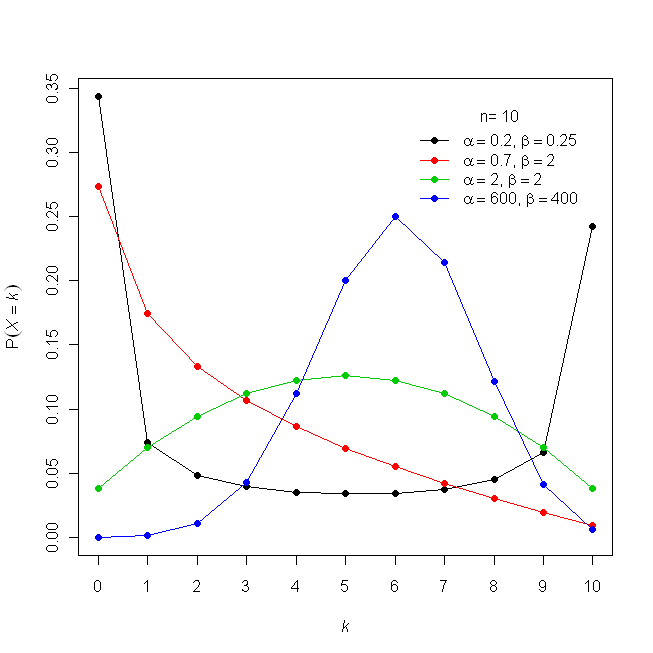
\includegraphics[width=0.8\linewidth]{../imagenes_marco_teorico/Beta-binomial_distribution.png}
    \caption{Distintas combinaciones de $\alpha$ y $\beta$ en la distribución beta binomial para n=10. Con $\alpha = 0.7$ y $\beta=2$ la distribución favorece los valores más bajos con un decaimiento hacia los más altos.}
\end{figure}

%\subsection{Fourier Gaussian Splatting}

Para la inicialización de gaussianas, una de las heurísticas abordadas en este trabajo se basa en la propuesta de FGS-SLAM \cite{xu2025fgsslamfourierbasedgaussiansplatting}. La idea central es usar información espectral para separar regiones con distinto nivel de detalle y, en función de ello, adaptar el muestreo y la escala de las gaussianas.

Sea $I(x,y)$ una imagen de tamaño $W \times H$. Su transformada discreta de Fourier (DFT) se define como:
\begin{equation}
F(u,v)=\sum_{x=0}^{W-1}\sum_{y=0}^{H-1} I(x,y)\, e^{-j2\pi(\frac{ux}{W}+\frac{vy}{H})}.
\end{equation}
En esta representación, las bajas frecuencias modelan variaciones suaves de intensidad, mientras que las altas frecuencias capturan bordes, texturas y cambios abruptos.

Siguiendo FGS-SLAM, se aplica un filtro pasa-altos gaussiano en el dominio de Fourier:
\begin{equation}
H(u,v)=1-e^{-\frac{D^2(u,v)}{2D_0^2}},
\end{equation}
donde $D(u,v)$ es la distancia al centro del espectro y $D_0$ controla la frecuencia de corte. La señal filtrada es:
\begin{equation}
F_h(u,v)=F(u,v)\,H(u,v),
\end{equation}
y la reconstrucción espacial de alta frecuencia se obtiene mediante la transformada inversa:
\begin{equation}
\tilde{I}_h(x,y)=\mathcal{F}^{-1}\{F_h(u,v)\}.
\end{equation}

En la implementación real del sistema, este proceso se ejecuta completamente en GPU. Primero se convierte la imagen RGB/BGRA a escala de grises de 8 bits. Luego se aplica FFT 2D real-compleja, filtrado pasa-altos sobre el espectro y FFT inversa. El parámetro de corte se implementa como
\begin{equation}
\sigma=\max\big(1,\,\rho\,\min(W,H)\big),
\end{equation}
donde $\rho$ es un parámetro de ratio a determinar empíricamente. Tras la reconstrucción, se toma la magnitud absoluta, se normaliza a $[0,255]$ y se construye un histograma de 256 bins.

Para separar regiones de alta y baja frecuencia se utiliza umbralización triangular sobre dicho histograma (consistente con la hipótesis unimodal tras el filtrado pasa-altos). Si $\tau$ es el umbral estimado, la máscara de alta frecuencia se define como:
\begin{equation}
M_h(x,y)=
\begin{cases}
1,& \tilde{I}_h(x,y)>\tau,\\
0,& \text{en otro caso,}
\end{cases}
\end{equation}
y la máscara de baja frecuencia como complemento:
\begin{equation}
M_l(x,y)=1-M_h(x,y).
\end{equation}

Estas máscaras se usan para densificación adaptativa: en regiones de alta frecuencia se emplea muestreo más denso y gaussianas de menor radio, mientras que en regiones de baja frecuencia se usa muestreo más espaciado y gaussianas de mayor radio. En términos de intervalos de muestreo, si $m$ corresponde a alta frecuencia y $n$ a baja frecuencia, se impone $m<n$.

Este mecanismo reduce la subrepresentación en zonas con detalle fino y, al mismo tiempo, evita sobrepoblar regiones homogéneas. No obstante, mantiene dos limitaciones inherentes al enfoque espectral: costo computacional $O(N\log N)$ y carácter global de la FFT (cada coeficiente depende de la imagen completa), lo que puede impactar latencia y localidad de decisión en escenarios estrictos de tiempo real.

En conclusión, la heurística de Fourier ofrece un criterio físicamente interpretable para distribuir gaussianas según complejidad local de la escena, y en este trabajo se adopta en una versión coherente con la implementación GPU del sistema.


%\section{Detección y cierre de ciclos}

\subsection{Submapas}

Implementamos el sistema de submapas propuesto en LoopSplat, realizando todas las operaciones que antes eran globales, como la optimización de las gaussianas en la imagen, en un marco local de cada submapa. De esta forma, cada submapa se construye a partir de un conjunto de fotogramas consecutivos, obteniendo así regiones reducidas. Si bien esto beneficia la eficiencia de las operaciones, reduce la ventaja del muestreo global de keyframes, ya que dos keyframes de submapas distintos no pueden ser comparados directamente. Esto quiere decir que la optimización pierde el mantenimiento global por sí sola. Sin embargo, en este marco el objetivo es el mantenimiento global a partir de los ciclos, enriqueciendo no solo la calidad de la representación, sino también la estimación de la pose.

\subsection{Descriptor}

Para la extracción del descriptor NetVLAD utilizamos la implementación en Python de HLoc \cite{sarlin2019coarse}, disponible en \url{https://github.com/cvg/Hierarchical-Localization} y la red preentrenada en el conjunto de datos Pitts30k, de forma análoga a LoopSplat. Esta versión de la red da lugar a descriptores de tamaño $4096$. Como nuestra implementación está escrita en C++, la integración con HLoc se realiza montando un servidor que contiene el código de extracción en Python. El cliente, es decir nuestro nodo, se comunica con el servidor entregándole la imagen a procesar y recibiendo el descriptor.

Esta implementación añade tiempos de latencia adicionales debido a los tiempos de comunicación, sin embargo, la arquitectura desacoplada de los hilos de detección de ciclos y el modelo de procesamiento por submapas permiten que esta latencia no afecte negativamente el rendimiento general del sistema. Además, facilita el acceso a posibles mejoras futuras en la red NetVLAD sin necesidad de reimplementaciones.

Es posible implementar este factor en un nodo separado de ROS2, realizando la comunicación a través de mensajes. Sin embargo, esto mantiene la latencia de comunicación, y abre la posibilidad de incompatibilidades entre las versiones de Python y dependencias entre ROS2 y HLoc. Por ello, se optó por una comunicación directa que, a su vez, permite optimizaciones en GPU.

\subsection{Heurísticas la detección de ciclos}

Para reducir el número de falsos positivos en la detección de ciclos, se implementan dos heurísticas principales. La primera es un filtro basado en la coherencia entre los centros de los submapas candidatos: si la distancia euclidiana entre los centros de las nubes de puntos de los submapas es mayor que un umbral predefinido, se descarta la correspondencia. Análogamente, si la orientación entre dos submapas no es coherente, también se descarta. La segunda heurística es el filtro por similaridad definido en el trabajo original.


\subsection{Registro de gaussianas}

En lugar de utilizar un método basado en los jacobianos de la renderización, optamos por un enfoque más clásico en SLAM basado en el registro de nubes de puntos. Para ello, reinterpretamos los centros de las gaussianas como puntos en el espacio 3D, y sus covarianzas como incertidumbres asociadas a cada punto. De esta forma, el problema de registro se convierte en un problema de alineación de nubes de puntos. Para resolverlo, empleamos una variante de ICP (\textit{Iterative Closest Point}) que tiene en cuenta las covarianzas, implementada en Open3D \cite{zhou2018open3dmodernlibrary3d}. Esta librería requiere una estimación inicial de la transformación, la cual obtenemos a partir de la pose estimada por la IMU.

\subsection{Optimización del grafo de poses}

Una vez obtenidas las correspondencias entre los submapas que cierran un ciclo, se construye un grafo de poses donde cada nodo representa la pose de un submapa y cada arista representa una restricción de transformación. Para optimizar este grafo, se utiliza la biblioteca Ceres Solver \cite{Agarwal_Ceres_Solver_2022}, que permite resolver problemas de optimización no lineal en CPU. Debido a la reducción del número de nodos como submapas, la optimización no se ve afectada significativamente por el rendimiento de la CPU.

%=========================================================

%%%%%%%%%%%%%%%%%%%%%%%%%%%%%%%%%%%%%
% ESTADO DEL ARTE
%%%%%%%%%%%%%%%%%%%%%%%%%%%%%%%%%%%%%
\chapter{Estado del arte}
\label{estado_del_arte}

% --------------------------------------------------
% SECCIONES
% --------------------------------------------------

\section{VIGS-Fusion}
El paper que inspiró este trabajo, llamado VIGS-Fusion \cite{ndoye2025vigs}, realizó una versión de Gaussian Splatting para reconstrucción tridimensional a partir de datos de una cámara RGB-D y una IMU. El trabajo fue preparado para ser implementado en un UAV pequeño a tiempo real, por lo que era fundamental una eficiencia temporal elevada y resultados robustos. 
A partir de plantear un problema de optimización que incluye los sesgos de la IMU, logró velocidades de reconstrucción de hasta 30x las del estado del arte para SLAM con estos sensores. La modificación principal frente a los demás métodos de la literatura es que presentó tanto un marco de corrección para los sesgos de la IMU, como distintos cálculos para los gradientes de las gaussianas.

\begin{figure}[H]
    \centering
    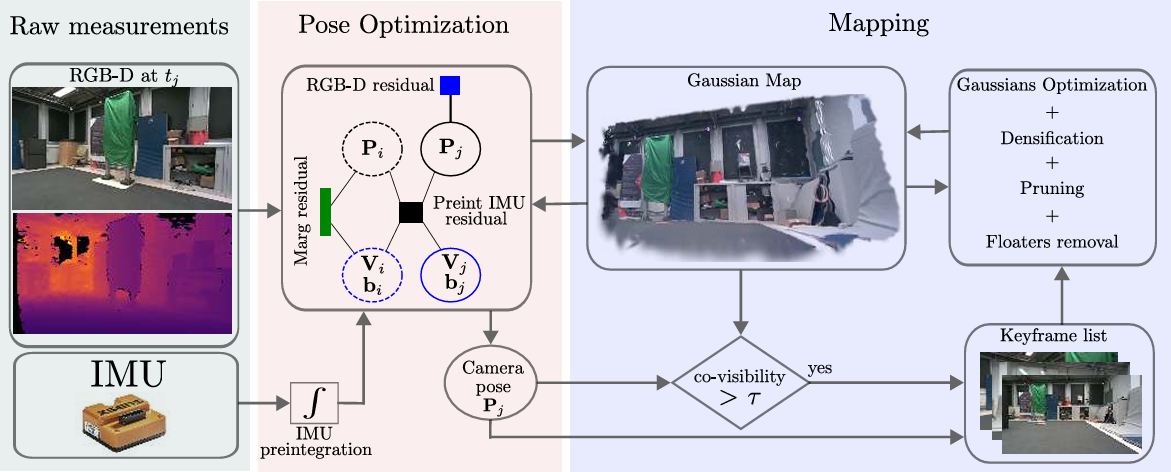
\includegraphics[width=0.75\linewidth]{../imagenes_marco_teorico/pipeline_vigs_fusion.png}
    \caption{Pipeline del paper VIGS-Fusion. Los keyframes son elegidos cuando la co-visibilidad con el frame actual supera un umbral $\tau$. En la optimización de la pose obtienen residuos de marginalización, de RGB-D y de la IMU.}
    \label{fig:pipeline_vigs_fusion}
\end{figure}

Ahora, veamos el método presentado por el paper.

\subsection{Optimización de la pose}

El estado a tiempo $k$ se define como

\begin{equation}
    x_k = [\mb{P}_k, \mb{V}_k, \mb{b}_a^k, \mb{b}_g^k]
\end{equation}

con $\mb{P}_k \in SE(3)$ representando la traslación $\mb{p}_k \in \mathbb{R}^3$ y la rotación $\mb{R}_k \in SO(3)$; $\mb{V}_k$ la velocidad; $\mb{b}_a^k$ y $\mb{b}_g^k$ los sesgos del acelerómetro y giróscopo, respectivamente.

Para optimizar, se define una función de costo general que combina los residuos de RGB-D, de IMU y de marginalización:

\begin{equation}
C(\mb{x}_k) = r_{RGB-D} + r_{IMU} + r_{Marg}
\end{equation}

Para la minimización se utilizó Levenberg-Marquadt, con una aproximación del segundo orden $r_{RGB-D}$, en contraste con los métodos del estado del arte que utilizaban descenso del gradiente de primer orden.

Para calcular el Jacobiano respecto de la pose $\mb{P}_k$, se planteó desde el álgebra de Lie, teniendo en cuenta que $\mb{P}_k \in SE(3)$ induce una representación $\xi_k = [\rho, \omega]^T \in \mathfrak{se}(3)$ con $\rho \in \mathbb{R}^3$ la traslación y $\omega \in \mathbb{R}^3$ la rotación. En este caso, la actualización se hace con perturbación a izquierda, porque el paper premultiplica el incremento al estado:

\begin{equation}
\mb{P}_{k+1} = \exp(\delta \xi)\,\mb{P}_k = \delta \xi \oplus_{\mathrm{izq}} \mb{P}_k
\end{equation}

Esta convención se conserva aquí para mantener la formulación original del método, pero queda explícito que la perturbación es a izquierda.

\subsection{Residuo RGB-D}
Este residuo se compone del residuo fotométrico, que es la diferencia entre el color observado y el renderizado, $r_{photo} = RGB(x) - C(x)$, y el residuo geométrico, que es la diferencia entre la profundidad observada y la renderizada, $r_{geo} = D(x) - d(x)$. Para calcular la profundidad renderizada $d(x)$ se consideró la mediana de las profundidades de las gaussianas calculadas con \ref{profundidad_gaussianas}.

\begin{equation}
r_{RGB-D} = r_{photo} + r_{geo}
\end{equation}

En la literatura, se utiliza descenso del gradiente computando el Jacobiano a partir del modelo de color y profundidad, requiriendo muchos parámetros para poder diferenciar la suma de gaussianas pesadas. En este paper, se determinó un cambio que consiste en usar las derivadas de la imagen observada en el espacio bidimensional. Para obtener los Jacobianos se diferenciaron el color observado $RGB(x)$ y la profundidad $D(x)$.

\subsubsection{Jacobiano del error fotométrico}

\begin{equation}
\mb{J}_{\xi_c}^{r_{photo}} = \frac{\mc{D}r_{photo}}{\mc{D}\xi_c} = 
\frac{\mc{D}(RGB(x) - C(x))}{\mc{D}\xi_c} = \frac{\mc{D}RGB(x)}{\mc{D}\xi_c}
\label{jacobiano_error_fotometrico}
\end{equation}

Utilizando los gradientes de la imagen observada, se aplicó la regla de la cadena

\begin{equation}
\frac{\mc{D}RGB(x)}{\mc{D}\xi_c} = \frac{\mc{D}RGB(x)}{\mc{D}\mb{u}} 
\frac{\mc{D}\mb{u}}{\mc{D}\mb{u}_c} \frac{\mc{D}\mb{u}_c}{\mc{D}\xi_c}
\end{equation}

donde $\mb{u}(u_x, u_y)$ es la ubicación del píxel en el plano bidimensional, y $\mb{u}_c$ su ubicación en el espacio tridimensional en el sistema de referencia de la cámara.

A partir de esta descomposición, se tienen los siguientes términos:

\begin{itemize}
    \item 
    El gradiente de la imagen respecto de cada color y dirección:
    \begin{equation}
    \frac{\mc{D}RGB(x)}{\mc{D}\mb{u}} =
    \begin{bmatrix}
        g_{u_x}^R & g_{u_x}^G & g_{u_x}^B\\
        g_{u_y}^R & g_{u_y}^G & g_{u_y}^B
    \end{bmatrix} ^T
    \end{equation}
    donde $g_{u_a}^b$ representa el gradiente en la dirección $a$ del canal $b$.
    
    \item 
    El Jacobiano de la proyección de la cámara deducido en \ref{jacobiano_proyeccion_camara}.
    $\frac{\mc{D}\mb{u}}{\mc{D}\mb{u}_c} = \mb{J}_c$

    \item 
    El Jacobiano de los puntos respecto de un movimiento en la pose
    \begin{equation}
    \frac{\mc{D}\mb{u}_c}{\mc{D}\xi_c}
    \end{equation}
    Para encontrar una fórmula cerrada, \cite{Matsuki2024GaussianSplattingSLAM} utilizó la derivación en la variante. Así, la perturbación $\delta \xi_c$, descompuesta en su traslación $\rho'$ y su rotación $\omega'$ induce la acción sobre el punto
    
    \begin{equation}
    \mb{u}_c' = (\mb{I} + [\omega']_X) \mb{u}_c + \rho
    \end{equation}

    por lo que la perturbación lleva a la diferencia

    \begin{equation}
    \delta\mu_c = \mu_c' - \mu_c = \rho + [\omega]_X \mu_c = \rho - [\mu_c]_X \,\,\omega
    \end{equation}

    Luego, podemos expresar el Jacobiano como

    \begin{equation}
    \frac{\mc{D}\mb{u}_c}{\mc{D}\xi_c} = 
    \begin{bmatrix}
        \mb{I} & -[\mb{u}_c]_X
    \end{bmatrix}
    \label{jacobiano_puntos_pose}
    \end{equation}
\end{itemize}

\subsubsection{Jacobiano del error geométrico}

\begin{equation}
    \mb{J}_{\xi_c}^{r_{geo}} = \frac{\mc{D}(D(x) - d(x))}{\mc{D}\xi_c} = \frac{\mc{D}D(x)}{\mc{D}\xi_c}
\end{equation}

Mediante la regla de la cadena,

\begin{equation}
    \frac{\mc{D}D(x)}{\mc{D}\xi_c} = \frac{\mc{D}D(\mb{x})}{\mc{D}\mb{u}_c}
    \frac{\mc{D}\mb{u}_c}{\mc{D}\xi_c}
\end{equation}

De nuevo, tenemos una descomposición con los términos:

\begin{itemize}
    \item 
    La dirección del rayo. Despejando en \ref{proyeccion_pinhole}, surge que
    \begin{equation}
    \frac{\mc{D}D(\mb{x})}{\mc{D}\mb{u}_c} = r = 
    \begin{bmatrix}
        \frac{u_x - c_x}{f_x} \\
        \frac{u_y - c_y}{f_y}
    \end{bmatrix}
    \end{equation}

    \item 
    El Jacobiano de los puntos respecto de un movimiento en la pose, que ya calculamos en \ref{jacobiano_puntos_pose}
\end{itemize}



\subsubsection{Resultados para $r_{RGB-D}$}

Al plantear los residuos como una matriz de la forma

\begin{equation}
    \mb{r}_{RGB-D} =
    \begin{bmatrix}
        \mb{r}_{photo} \\
        \mb{r}_{geo}
    \end{bmatrix}
\end{equation}

se expresa el Jacobiano completo

\begin{equation}
    \mb{J}_{\xi_c}^{r_{RGB-D}} =
    \begin{bmatrix}
        \mb{J}_{\xi_c}^{r_{photo}} \\
        \mb{J}_{\xi_c}^{r_{geo}}
    \end{bmatrix}
\end{equation}

Luego, para poder usar Levenberg-Marquadt se tienen las expresiones

\begin{equation}
    {\mb{J}_{\xi_c}^{r_{RGB-D}}}^T \mb{J}_{\xi_c}^{r_{RGB-D}} =
    {\mb{J}_{\xi_c}^{r_{photo}}}^T \mb{J}_{\xi_c}^{r_{photo}} +
    {\mb{J}_{\xi_c}^{r_{geo}}}^T \mb{J}_{\xi_c}^{r_{geo}}
\end{equation}
    
\begin{equation}
    {\mb{J}_{\xi_c}^{r_{RGB-D}}}^T \mb{r}_{RGB-D} =
    {\mb{J}_{\xi_c}^{r_{photo}}}^T \mb{r}_{photo} +
    {\mb{J}_{\xi_c}^{r_{geo}}}^T \mb{r}_{geo}
\end{equation}


%%%%%%%%%%%%%%%%%%%%%%%%%

\subsection{Residuo IMU}

El estado del sistema en el instante $k$ se define como

\begin{equation}
\mathbf{x}_k =
\left(
\mathbf{p}_k,
\mathbf{q}_k,
\mathbf{v}_k,
\mathbf{b}_{a_k},
\mathbf{b}_{g_k}
\right)
\end{equation}

donde $\mathbf{p}_k$ es la posición, $\mathbf{q}_k$ la orientación, $\mathbf{v}_k$ la velocidad y $\mathbf{b}_{a_k},\mathbf{b}_{g_k}$ representan los sesgos del acelerómetro y el giroscopio respectivamente.

Entre dos fotogramas consecutivos $i$ y $j$, las mediciones de la IMU se preintegran obteniendo las cantidades

\begin{equation}
(\Delta \mathbf{p}_{ij}, \Delta \mathbf{v}_{ij}, \Delta \mathbf{q}_{ij})
\end{equation}

que representan los cambios relativos de posición, velocidad y orientación expresados en el sistema de referencia del instante $i$.

Siguiendo la formulación de la preintegración en variedades, la predicción del estado en el instante $j$ a partir del estado en $i$ puede escribirse como

\begin{align}
\mathbf{p}_j &=
\mathbf{p}_i
+
\mathbf{v}_i \Delta t
+
\frac12 \mathbf{g} \Delta t^2
+
\mathbf{R}_i
\Delta \mathbf{p}_{ij}
\\
\mathbf{v}_j &=
\mathbf{v}_i
+
\mathbf{g}\Delta t
+
\mathbf{R}_i
\Delta \mathbf{v}_{ij}
\\
\mathbf{q}_j &=
\mathbf{q}_i
\otimes
\Delta \mathbf{q}_{ij}
\end{align}

donde $\mathbf{R}_i$ es la matriz de rotación asociada al cuaternión $\mathbf{q}_i$.

El residuo IMU compara la predicción obtenida mediante estas ecuaciones con el estado estimado por el optimizador. Se define entonces como

\begin{equation}
\mathbf{r}_{IMU}
=
\begin{bmatrix}
\mathbf{r}_p \\
\mathbf{r}_q \\
\mathbf{r}_v \\
\mathbf{r}_{ba} \\
\mathbf{r}_{bg}
\end{bmatrix}
\end{equation}

donde cada componente corresponde a un error en posición, orientación, velocidad y sesgos.

El residuo de posición se define como

\begin{equation}
\mathbf{r}_p =
\mathbf{R}_i^\top
\left(
\mathbf{p}_j
-
\mathbf{p}_i
-
\mathbf{v}_i \Delta t
-
\frac12 \mathbf{g}\Delta t^2
\right)
-
\Delta \mathbf{p}_{ij}
\end{equation}

El residuo de velocidad se expresa como

\begin{equation}
\mathbf{r}_v =
\mathbf{R}_i^\top
\left(
\mathbf{v}_j
-
\mathbf{v}_i
-
\mathbf{g}\Delta t
\right)
-
\Delta \mathbf{v}_{ij}
\end{equation}

Para la orientación se utiliza la diferencia de cuaterniones en el grupo $SO(3)$

\begin{equation}
\mathbf{r}_q =
(\mathbf{q}_i^{-1}\mathbf{q}_j)
\ominus
\Delta\mathbf{q}_{ij}
\end{equation}

Utilizando la parametrización mínima del error rotacional en $SO(3)$, este término puede escribirse explícitamente como

\begin{equation}
\mathbf{r}_q =
2\,\mathrm{vec}
\left(
\Delta \mathbf{q}_{ij}^{-1}
(\mathbf{q}_i^{-1}\mathbf{q}_j)
\right).
\end{equation}

donde $\mathrm{vec}(\cdot)$ extrae la parte vectorial del cuaternión.

Los residuos asociados a los sesgos se definen como

\begin{align}
\mathbf{r}_{ba} &= \mathbf{b}_{a_j} - \mathbf{b}_{a_i} \\
\mathbf{r}_{bg} &= \mathbf{b}_{g_j} - \mathbf{b}_{g_i}
\end{align}

Para resolver el problema mediante optimización no lineal, el residuo se linealiza alrededor de una estimación actual $\tilde{\mathbf{x}}$.

\begin{equation}
\mathbf{r}_{IMU}(\mathbf{x})
\approx
\mathbf{r}_{IMU}(\tilde{\mathbf{x}})
+
\mathbf{J}
\delta \mathbf{x}
\end{equation}

donde

\begin{equation}
\mathbf{J}
=
\frac{\partial \mathbf{r}_{IMU}}{\partial \mathbf{x}}
\end{equation}

es el Jacobiano del residuo respecto al estado.

Por ejemplo, derivando el residuo de posición respecto a $\mathbf{p}_i$ se obtiene

\begin{equation}
\frac{\partial \mathbf{r}_p}{\partial \mathbf{p}_i}
=
-\mathbf{R}_i^\top
\end{equation}

mientras que respecto a $\mathbf{p}_j$

\begin{equation}
\frac{\partial \mathbf{r}_p}{\partial \mathbf{p}_j}
=
\mathbf{R}_i^\top
\end{equation}

y respecto a la velocidad inicial

\begin{equation}
\frac{\partial \mathbf{r}_p}{\partial \mathbf{v}_i}
=
-\mathbf{R}_i^\top \Delta t
\end{equation}

Las derivadas respecto a la orientación utilizan la aproximación de primer orden de la rotación

\begin{equation}
\mathbf{R}(\delta \boldsymbol{\theta})
\approx
\mathbf{I}
+
[\delta \boldsymbol{\theta}]_\times
\end{equation}

Finalmente, los residuos se ponderan mediante la matriz de información de la medición

\begin{equation}
\|r\|^2 =
\mathbf{r}_{IMU}^\top
\mathbf{W}
\mathbf{r}_{IMU}
\end{equation}

donde $\mathbf{W}=\boldsymbol{\Sigma}^{-1}$ es la inversa de la covarianza de la preintegración.



%%%%%%%%%%%%%%%%%%%%%%%%%%%%%%%%%%%%%%%%%%%%%%%
\subsection{Residuo de marginalización}

Al obtener nuevos datos, el sistema estima un nuevo estado $\mathbf{x}_k$. 
Para mantener el problema de optimización computacionalmente manejable, se utiliza 
una estrategia de \textit{ventana deslizante}, donde los estados más antiguos se eliminan 
de la optimización. Sin embargo, eliminar directamente dichos estados implicaría perder 
la información contenida en las mediciones asociadas a ellos. 

Para evitar esta pérdida de información, se realiza un proceso de \textit{marginalización}, 
mediante el cual las variables antiguas se eliminan del problema pero su información se 
condensa en un nuevo factor que actúa como un prior sobre las variables restantes.

Sea el vector completo de variables del problema

\begin{equation}
\mathbf{x} =
\begin{bmatrix}
\mathbf{x}_m \\
\mathbf{x}_r
\end{bmatrix}
\end{equation}

donde

\begin{itemize}
\item $\mathbf{x}_m$ representa las variables que se desean marginalizar (estados antiguos),
\item $\mathbf{x}_r$ representa las variables que permanecerán en la optimización.
\end{itemize}

El problema de mínimos cuadrados puede escribirse como

\begin{equation}
\min_{\mathbf{x}}
\|\mathbf{r}(\mathbf{x})\|^2
\end{equation}

donde $\mathbf{r}(\mathbf{x})$ es el vector de residuos del sistema.

Linealizando alrededor de una estimación actual $\tilde{\mathbf{x}}$ se obtiene

\begin{equation}
\mathbf{r}(\mathbf{x})
\approx
\mathbf{r}_0 + \mathbf{J}\delta\mathbf{x}
\end{equation}

donde

\begin{equation}
\delta\mathbf{x} =
\mathbf{x} \ominus \tilde{\mathbf{x}}
\end{equation}

y $\mathbf{J}$ es el Jacobiano del residuo.

El sistema normal asociado al problema de mínimos cuadrados es

\begin{equation}
\mathbf{A}\delta\mathbf{x} = \mathbf{b}
\end{equation}

con

\begin{align}
\mathbf{A} &= \mathbf{J}^\top \mathbf{J} \\
\mathbf{b} &= \mathbf{J}^\top \mathbf{r}_0
\end{align}

Separando las variables a marginalizar y las variables restantes, la matriz 
$\mathbf{A}$ puede escribirse como

\begin{equation}
\mathbf{A} =
\begin{bmatrix}
\mathbf{A}_{mm} & \mathbf{A}_{mr} \\
\mathbf{A}_{rm} & \mathbf{A}_{rr}
\end{bmatrix}
\end{equation}

y el vector $\mathbf{b}$ como

\begin{equation}
\mathbf{b} =
\begin{bmatrix}
\mathbf{b}_m \\
\mathbf{b}_r
\end{bmatrix}.
\end{equation}

Para eliminar las variables $\mathbf{x}_m$ se aplica el complemento de Schur, 
obteniéndose un nuevo sistema reducido

\begin{align}
\mathbf{A}^\ast &= 
\mathbf{A}_{rr} -
\mathbf{A}_{rm}
\mathbf{A}_{mm}^{-1}
\mathbf{A}_{mr}
\\
\mathbf{b}^\ast &=
\mathbf{b}_r -
\mathbf{A}_{rm}
\mathbf{A}_{mm}^{-1}
\mathbf{b}_m
\end{align}

que depende únicamente de las variables restantes $\mathbf{x}_r$.

Este sistema reducido define un nuevo factor que encapsula la información de las 
variables marginalizadas.

Para integrarlo nuevamente en el optimizador, se busca una factorización de la forma

\begin{equation}
\mathbf{A}^\ast =
\mathbf{J}_{marg}^\top
\mathbf{J}_{marg}
\end{equation}

donde $\mathbf{J}_{marg}$ es el jacobiano del nuevo factor de marginalización.

En la implementación, esta factorización se obtiene mediante descomposición espectral

\begin{equation}
\mathbf{A}^\ast =
\mathbf{V}
\mathbf{\Lambda}
\mathbf{V}^\top
\end{equation}

de donde se define

\begin{equation}
\mathbf{J}_{marg} =
\sqrt{\mathbf{\Lambda}}
\mathbf{V}^\top .
\end{equation}

El residuo asociado al factor de marginalización se define entonces como

\begin{equation}
\mathbf{r}_{marg}(\mathbf{x}_r)
=
\mathbf{r}_0
+
\mathbf{J}_{marg}
\delta\mathbf{x}_r
\end{equation}

donde

\begin{equation}
\mathbf{r}_0 =
\mathbf{J}_{marg}^{-T}
\mathbf{b}^\ast .
\end{equation}

Finalmente, el incremento de estado utilizado en la evaluación del residuo es

\begin{equation}
\delta\mathbf{x}_r =
\mathbf{x}_r \ominus \mathbf{x}_r^0
\end{equation}

donde $\mathbf{x}_r^0$ es el punto de linearización almacenado en el momento de 
realizar la marginalización.

En el caso de variables definidas en $SE(3)$, el incremento se calcula en el 
espacio tangente. Para una pose representada por posición $\mathbf{p}$ y 
cuaternión $\mathbf{q}$ se utiliza

\begin{equation}
\delta\mathbf{x} =
\begin{bmatrix}
\mathbf{p}-\mathbf{p}_0 \\
2\,\mathrm{vec}
\left(
\mathbf{q}_0^{-1}\mathbf{q}
\right)
\end{bmatrix}.
\end{equation}

De esta manera, el factor de marginalización actúa como un prior gaussiano 
sobre las variables restantes, preservando la información de los estados 
eliminados mientras se mantiene constante el tamaño del problema de optimización.




%%%%%%%%%%%%%%%%%%%%%%%%%%%%%%%%%%%%%%%%%%%%%%%%%%%%%%%%%%%%%%%%%%%%%%%%%%%%%%%%

\subsection{Función de costo para gaussianas}

En este trabajo se utiliza una función de costo compuesta por tres términos, análoga a la de otros trabajos como RAD-GS \cite{radgs}:

\begin{equation}
\mathcal{L} = \mathcal{L}_{\text{rgb}} + w_{\text{depth}} \mathcal{L}_{\text{depth}} + w_{\text{dist}} \mathcal{L}_{\text{dist}} + \lambda_{\text{iso}} \mathcal{L}_{\text{iso}}
\end{equation}

donde:

\paragraph{Término fotométrico ($\mathcal{L}_{\text{rgb}}$):}
Mide la diferencia cuadrática entre el color renderizado y el observado en cada píxel:
\begin{equation}
\mathcal{L}_{\text{rgb}} = \sum_{p} \frac{1}{2}\|C(p) - C^*(p)\|_2^2
\end{equation}
con $C(p) = \sum_n T_n \alpha_n c_n$ el color renderizado mediante alpha-blending ordenado en profundidad.

\paragraph{Término de profundidad mediana ($\mathcal{L}_{\text{depth}}$):}
Penaliza la diferencia entre la profundidad renderizada en el punto mediano de transmitancia (cuando $T$ cruza 0.5) y la profundidad observada:
\begin{equation}
\mathcal{L}_{\text{depth}} = \sum_{p} \frac{w_{\text{depth}}}{2}\, \mathbf{1}_{\text{med}}(p)\, \big(D_{\text{med}}(p) - D^*(p)\big)^2
\end{equation}
donde $\mathbf{1}_{\text{med}}(p)$ es un indicador que vale 1 en el splat donde la transmitancia cruza 0.5, y la profundidad en ese punto es:
\begin{equation}
D_{\text{med}}(p) = z_n + \hat{p}_n \cdot (p - \mu_n^{2D})
\end{equation}
con $\hat{p}_n$ el vector que codifica cómo varía la profundidad con el desplazamiento en imagen.

\paragraph{Término de distorsión de profundidad ($\mathcal{L}_{\text{dist}}$):}
Regulariza la consistencia entre la profundidad de cada splat y la profundidad mediana acumulada, pesando por la contribución de cada gaussiana:
\begin{equation}
\mathcal{L}_{\text{dist}} = \sum_{p,n} \frac{w_{\text{dist}}}{2}\, \alpha_n(p)\,T_n(p)\, \big(d_n(p)-D_{\text{med}}(p)\big)^2
\end{equation}
donde $d_n(p) = z_n + \hat{p}_n \cdot (p - \mu_n^{2D})$ es la profundidad de la gaussiana $n$ en el píxel $p$.

\paragraph{Término de regularización isotrópica ($\mathcal{L}_{\text{iso}}$):}

Penaliza que las gaussianas sean muy anisótropas (muy alargadas en una dirección), favoreciendo formas más esféricas:

\begin{equation}
\mathcal{L}_{\text{iso}} = \sum_{n} \lambda_{\text{iso}}\sum_{i} (s_{n,i} - \bar{s}_n)^2
\end{equation}
donde $s_{n,i}$ son las componentes de escala de la gaussiana $n$ y $\bar{s}_n = (s_{n,x} + s_{n,y} + s_{n,z})/3$.

Esta formulación permite balancear la fidelidad fotométrica con restricciones geométricas provenientes de sensores RGB-D, crucial para mantener una reconstrucción métrica consistente en SLAM visual.




\subsection{Gradientes}

Dada la función de costo, ahora podemos calcular los gradientes respecto de los parámetros de las gaussianas. Para esto, VIGS-Fusion plantea cálculo sobre las imágenes proyectadas, simplificando el costo computacional de las derivadas. A continuación, se detallan los cálculos para cada tipo de parámetro.

\subsubsection{Gradiente de color}

El color se forma a partir del alpha-blending de los splats bidimensionales. Por tanto,

\begin{equation}
C = \sum_n T_n \alpha_n c_n
\end{equation}

con $T_n$ la transmitancia, $\alpha_n$ la opacidad y $c_n$ el color de la gaussiana $n$ en orden de profundidad back-to-front.

Luego, tenemos que, sea $e = C - C_{obs}$ tal que $L = \frac{1}{2}||e||^2$ sea la función de pérdida,

\begin{equation}
    \frac{\partial L}{\partial c_n} = 
    \frac{\partial L}{\partial C} \frac{\partial C}{\partial c_n} =
    e (T_n\alpha_n)
\end{equation}

Ahora, para poder extenderlo a la gaussiana tridimensional, no es necesario realizar ningún cambio, ya que el color no se perturba al proyectar. Podemos simplemente usar

\begin{equation}
    \frac{\partial L}{\partial c_n^{3d}} = \frac{\partial L}{\partial c_n^{2d}}
\end{equation}



\subsubsection{Gradiente de opacidad}

Para la opacidad $\alpha_n$, tenemos que la misma influye activamente en el término correspondiente a la gaussiana $n$, y en todas las posteriores a partir del alpha-blending, pues

\begin{equation}
T_n = \prod_{k<n}(1-\alpha_k) 
\end{equation}

Al derivar, tenemos tanto el término propio de color $T_n \alpha_n c_n$ como todos los términos posteriores. Como el término propio es lineal en $\alpha_n$, la derivada es simplemente $T_n c_n$. Por otro lado, para un $m>n$ fijo,

\begin{equation}
\frac{\partial T_m}{\partial \alpha_n} = - \frac{T_m}{1 - \alpha_n}
\end{equation}

Luego,

\begin{equation}
    \frac{\partial C}{\partial \alpha_n} = T_nc_n - \frac{1}{1-\alpha_n} \sum_{m>n}T_m\alpha_mc_m
    = T_n c_n - \frac{C - C_{\leq n}}{1-\alpha_n}
\end{equation}

con $C_{\leq n}$ el color acumulado hasta n.

Finalmente,

\begin{equation}
    \frac{\partial L}{\partial \alpha_n} = 
    \frac{\partial L}{\partial C} \frac{\partial C}{\partial \alpha_n} =
    e (T_n c_n - \frac{C - C_{\leq n}}{1-\alpha_n})
\end{equation}


\subsubsection{Gradiente de la media}

Para calcular el gradiente de la media $\mu_{3D}$, lo separamos en:

\begin{equation}
    \frac{\partial L}{\partial \mu_{3D}} =
    \frac{\partial L}{\partial \mu_{2D}} \frac{\partial \mu_{2D}}{\partial \mu_{3D}}
    + \frac{\partial L}{\partial z} \frac{\partial z}{\partial \mu_{3D}}
    + \frac{\partial L}{\partial \Sigma'} \frac{\partial \Sigma'}{\partial \mu_{3D}}
\end{equation}

Ahora, deducimos cada término

\paragraph{Media bidimensional}

Sea $\mb{J}$ el jacobiano de la proyección,

\begin{equation}
    \frac{\partial \mu_{2D}}{\partial \mu_{3D}} = \mb{J}
\end{equation}

Para el factor restante, observamos que la media bidimensional influye en la
pérdida a través del peso gaussiano proyectado. Sea

\begin{equation}
G(x) =
\exp\!\left(
-\frac{1}{2} (x-\mu_{2D})^T \Sigma'^{-1} (x-\mu_{2D})
\right),
\end{equation}

y sea $\alpha = \sigma G$ la opacidad efectiva del splat en el píxel.
Entonces,

\begin{equation}
\frac{\partial \alpha}{\partial \mu_{2D}}
=
\alpha \, \Sigma'^{-1}(x-\mu_{2D}).
\end{equation}

Aplicando regla de la cadena,

\begin{equation}
\frac{\partial L}{\partial \mu_{2D}}
=
\frac{\partial L}{\partial \alpha}
\frac{\partial \alpha}{\partial \mu_{2D}}
=
\frac{\partial L}{\partial \alpha}
\alpha
\Sigma'^{-1}(x-\mu_{2D}).
\end{equation}

\paragraph{Profundidad}

La coordenada de profundidad es simplemente la tercera componente de la media en el sistema de referencia de la cámara:

\begin{equation}
    z = \mu_{3D,z}
\end{equation}

Por lo tanto,

\begin{equation}
    \frac{\partial z}{\partial \mu_{3D}} =
    \begin{bmatrix}
        0 & 0 & 1
    \end{bmatrix}
\end{equation}

y el término correspondiente del gradiente queda

\begin{equation}
    \frac{\partial L}{\partial z}
    \frac{\partial z}{\partial \mu_{3D}}
    =
    \frac{\partial L}{\partial z}
    \begin{bmatrix}
        0 & 0 & 1
    \end{bmatrix}.
\end{equation}

Para obtener $\frac{\partial \mathcal{L}}{\partial z}$, observamos que la profundidad aparece en dos lugares de la función de costo:

\paragraph{Deducción del gradiente del término de profundidad mediana}

El término de profundidad mediana es:
\begin{equation}
\mathcal{L}_{\text{depth}} = \sum_{p} \frac{w_{\text{depth}}}{2}\, \mathbf{1}_{\text{med}}(p)\, \big(D_{\text{med}}(p) - D^*(p)\big)^2
\end{equation}

Recordando que $D_{\text{med}}(p) = z_n + \hat{p}_n \cdot (p - \mu_n^{2D})$ para la gaussiana $n$ donde $T$ cruza 0.5, derivamos respecto a $z_n$:

\begin{equation}
\begin{split}
\frac{\partial \mathcal{L}_{\text{depth}}}{\partial z_n} &= \sum_{p} w_{\text{depth}} \, \mathbf{1}_{\text{med}}(p) \, \big(D_{\text{med}}(p) - D^*(p)\big) \frac{\partial D_{\text{med}}(p)}{\partial z_n} \\
&= \sum_{p} w_{\text{depth}} \, \mathbf{1}_{\text{med}}(p) \, \big(D_{\text{med}}(p) - D^*(p)\big) \cdot 1 \\
&= w_{\text{depth}} \, \mathbf{1}_{\text{med}}(n) \, (D_{\text{med}} - D^*)
\end{split}
\end{equation}

donde el indicador $\mathbf{1}_{\text{med}}(n)$ vale 1 únicamente en el píxel donde la gaussiana $n$ cruza $T=0.5$, y $\frac{\partial D_{\text{med}}}{\partial z_n} = 1$ ya que $D_{\text{med}}$ depende linealmente de $z_n$.

\paragraph{Deducción del gradiente del término de distorsión}

El término de distorsión es:
\begin{equation}
\mathcal{L}_{\text{dist}} = \sum_{p,n} \frac{w_{\text{dist}}}{2}\, \alpha_n(p)\,T_n(p)\, \big(d_n(p)-D_{\text{med}}(p)\big)^2
\end{equation}

Derivando respecto a $z_n$ (la profundidad de la gaussiana $n$):

\begin{equation}
\begin{split}
\frac{\partial \mathcal{L}_{\text{dist}}}{\partial z_n} &= \sum_{p} w_{\text{dist}} \, \alpha_n(p)\,T_n(p)\, \big(d_n(p) - D_{\text{med}}(p)\big) \frac{\partial d_n(p)}{\partial z_n} \\
&= \sum_{p} w_{\text{dist}} \, \alpha_n(p) \, T_n(p) \, (d_n(p) - D_{\text{med}}(p)) \cdot 1 \\
&= \sum_p w_{\text{dist}} \, \alpha_n(p) \, T_n(p) \, (d_n(p) - D_{\text{med}}(p))
\end{split}
\end{equation}

donde usamos que $d_n(p) = z_n + \hat{p}_n \cdot (p - \mu_n^{2D})$, de modo que $\frac{\partial d_n(p)}{\partial z_n} = 1$. 


En esta derivación, $D_{\text{med}}(p)$ se trata como constante respecto a $z_n$ mediante un \textit{stop-gradient}, es decir, considerando nulo el gradiente. Esto es correcto porque: (1) si $n$ no es el splat mediano en el píxel $p$, entonces $D_{\text{med}}(p)$ efectivamente depende de otro splat diferente, no de $z_n$; (2) si $n$ \emph{es} el splat mediano, ambas derivadas $\frac{\partial d_n}{\partial z_n} = 1$ y $\frac{\partial D_{\text{med}}}{\partial z_n} = 1$ se cancelarían, resultando en contribución nula.


\paragraph{Gradiente total respecto a la profundidad}

Por lo tanto, el gradiente total respecto a la profundidad es:
\begin{equation}
\frac{\partial \mathcal{L}}{\partial z_n} = \frac{\partial \mathcal{L}_{\text{depth}}}{\partial z_n} + \frac{\partial \mathcal{L}_{\text{dist}}}{\partial z_n}
\end{equation}

Este gradiente se acumula sobre todos los píxeles donde la gaussiana $n$ tiene contribución significativa, aplicándose el primer término solo en el píxel mediano y el segundo en todos los píxeles.



\paragraph{Covarianza proyectada}

Recordemos que la covarianza proyectada se describe en términos de la covarianza como

\begin{equation}
    \Sigma' = \mb{J} \, \Sigma \, \mb{J}^T
\end{equation}

donde $\mb{J}$ depende de la media 3D a través de la proyección perspectiva.

Luego, al derivar respecto de la media

\begin{equation}
    \frac{\partial \Sigma'}{\partial \mu_{3D}} = 
    \frac{\partial (\mb{J} \Sigma \mb{J}^T)}{\partial \mu_{3D}} =
    \frac{\partial \mb{J}}{\partial \mu_{3D}} \Sigma \mb{J} ^T 
    + \mb{J} \Sigma \frac{\partial \mb{J}^T}{\partial \mu_{3D}}
\end{equation}

Como consideramos la proyección afín local para todas las cuentas, se considera que el jacobiano es constante, dando lugar a que

\begin{equation}
    \frac{\partial \mb{J}}{\partial \mu_{3D}} \approx 0
\end{equation}

Luego, este término se anula.



\subsubsection{Gradientes respecto a Covarianza, Escala y Rotación}

Recordemos la parametrización de la covarianza en el sistema de referencia del mundo:

\begin{equation}
\Sigma = R S^2 R^T
\end{equation}

donde:
\begin{itemize}
    \item $R \in SO(3)$ es la matriz de rotación (obtenida del cuaternión),
    \item $S = \mathrm{diag}(s_x, s_y, s_z)$ contiene las escalas.
\end{itemize}

En esta formulación, la covarianza proyectada $\Sigma'$ resulta

\begin{equation}
\Sigma = \mb{T} \Sigma_{3D} \mb{T}^T
\end{equation}

donde:

\begin{equation}
T = J W
\end{equation}

y:
\begin{itemize}
    \item $J$ es el Jacobiano de proyección perspectiva,
    \item $W$ es la rotación cámara-mundo.
\end{itemize}

En lugar de optimizar directamente la covarianza 3D $\Sigma$, se parametrizan la rotación y la escala, para asegurarse de que la matriz resultante simétrica definida positiva, además de que brinda un sentido geométrico más sólido. Sin embargo, para calcular estos gradientes, es necesario, también, calcular el de la covarianza.

\paragraph{Gradiente respecto a la covarianza 3D}

Aplicando la regla de la cadena:

\begin{equation}
\frac{\partial \mathcal{L}}{\partial \Sigma_{3D}}
=
\mb{T}^T
\frac{\partial \mathcal{L}}{\partial \Sigma'}
\mb{T}
\end{equation}

Para obtener $\frac{\partial \mathcal{L}}{\partial \Sigma'}$, notamos que la covarianza 2D afecta a la pérdida a través de la forma gaussiana y, por tanto, de la opacidad $\alpha_n(p) = \sigma_n \exp(-\frac{1}{2}\delta^T \Sigma'^{-1} \delta)$, donde $\delta = p - \mu_n^{2D}$.

Usamos la identidad para la derivada de una inversa:
\begin{equation}
\frac{\partial F}{\partial A}
=
- A^{-T}
\frac{\partial F}{\partial A^{-1}}
A^{-T}
\end{equation}

Luego:
\begin{equation}
\frac{\partial \mathcal{L}}{\partial \Sigma'} = - \Sigma'^{-1} \frac{\partial \mathcal{L}}{\partial \Sigma'^{-1}} \Sigma'^{-1}
\end{equation}

Observando que:
\begin{equation}
\frac{\partial G}{\partial \Sigma'^{-1}} = -\frac{1}{2} G \, \delta \delta^T
\end{equation}

y

\begin{equation}
    \frac{\partial \alpha}{\partial G} = \sigma
\end{equation}

Aplicando la regla de la cadena, cadena:
\begin{equation}
\frac{\partial \mathcal{L}}{\partial \Sigma'^{-1}} = \frac{\partial \mathcal{L}}{\partial \alpha} \frac{\partial \alpha}{\partial G} \frac{\partial G}{\partial \Sigma'^{-1}} = 
-\frac{1}{2} \frac{\partial \mathcal{L}}{\partial \alpha} \, \sigma\, G\, \delta \delta^T
= -\frac{1}{2} \frac{\partial \mathcal{L}}{\partial \alpha} \, \alpha\, \delta \delta^T
\end{equation}

Este último paso surge de que $\alpha = \sigma G$

Este gradiente se acumula sobre todos los píxeles donde la gaussiana contribuye.



\paragraph{Gradiente respecto a la escala}

Sea $M \coloneq \mb{R} \mb{S}$, entonces

\begin{equation}
\Sigma_{3D} = M M^T
\end{equation}

El gradiente respecto a $M$ es:

\begin{equation}
\frac{\partial \mathcal{L}}{\partial M}
= 2 \frac{\partial \mathcal{L}}{\partial \Sigma} M
\end{equation}

Luego, por definición de $M$, el gradiente para la escala es

\begin{equation}
\frac{\partial \mathcal{L}}{\partial s_i}
=
R_{:,i}^T
\left(
\frac{\partial \mathcal{L}}{\partial M}
\right)_{:,i}
\end{equation}

Es posible expresar las escalas en logaritmo, en tal caso:

\begin{equation}
s_i = e^{\tilde{s}_i}
\end{equation}

entonces:

\begin{equation}
\frac{\partial \mathcal{L}}{\partial \tilde{s}_i}
=
\frac{1}{s_i}
\frac{\partial \mathcal{L}}{\partial s_i}
\end{equation}

\paragraph{Regularización isotrópica}

Para mantener una relación entre las escalas, se introduce un término de pérdida que depende solo de la escala:

\begin{equation}
\mathcal{L}_{iso}
=
\lambda_{iso}
\sum_i (s_i - \bar{s})^2
\end{equation}

donde:

\begin{equation}
\bar{s} = \frac{s_x + s_y + s_z}{3}
\end{equation}

Su gradiente es:

\begin{equation}
\frac{\partial \mathcal{L}_{iso}}{\partial s}
=
\frac{\lambda_{iso}}{3}
\begin{bmatrix}
2\Delta_x - \Delta_y - \Delta_z \\
-\Delta_x + 2\Delta_y - \Delta_z \\
-\Delta_x - \Delta_y + 2\Delta_z
\end{bmatrix}
\end{equation}

donde $\Delta_i = s_i - \bar{s}$.


\paragraph{Gradiente respecto a la rotación}

Recordemos que la covarianza se parametriza como

Aplicando regla de la cadena sobre $M = RS$,

\begin{equation}
\frac{\partial \mathcal{L}}{\partial R}
=
\frac{\partial \mathcal{L}}{\partial M} S .
\end{equation}

Sin embargo, $R \in SO(3)$, por lo que su gradiente debe proyectarse al
espacio tangente del grupo. Las variaciones admisibles de $R$ pueden
escribirse como

\begin{equation}
dR = R[\delta\theta]_\times ,
\end{equation}

Utilizando esta parametrización y propiedades del producto traza, se obtiene
que el gradiente respecto al vector de rotación viene dado por

\begin{equation}
\frac{\partial \mathcal{L}}{\partial \theta}
=
-
\sum_{i=1}^{3}
R_{:,i}
\times
\left(
\frac{\partial \mathcal{L}}{\partial R}
\right)_{:,i}.
\end{equation}

\subsubsection{Peso por relevancia}

En la práctica, es conveniente mantener proporcionalmente más estáticas a las gaussianas que participan en más píxeles, y menos a las que no. Debido a esto, se define un factor que depende de la cantidad de observaciones $n$ de la gaussiana

\begin{equation}
    \eta = \eta(n) \coloneq \frac{1}{5 + n}
\end{equation}

El mismo se multiplica al gradiente real antes de pasarlo al algoritmo de optimización. Notemos que, a mayor $n$, menor $\eta$, por lo que el gradiente será más bajo y tenderá a modificarse menos en la iteración del optimizador.

\subsection{Fourier Gaussian Splatting}

Para la inicialización de gaussianas, una de las heurísticas abordadas en este trabajo se basa en la propuesta de FGS-SLAM \cite{xu2025fgsslamfourierbasedgaussiansplatting}. La idea central es usar información espectral para separar regiones con distinto nivel de detalle y, en función de ello, adaptar el muestreo y la escala de las gaussianas.

Sea $I(x,y)$ una imagen de tamaño $W \times H$. Su transformada discreta de Fourier (DFT) se define como:
\begin{equation}
F(u,v)=\sum_{x=0}^{W-1}\sum_{y=0}^{H-1} I(x,y)\, e^{-j2\pi(\frac{ux}{W}+\frac{vy}{H})}.
\end{equation}
En esta representación, las bajas frecuencias modelan variaciones suaves de intensidad, mientras que las altas frecuencias capturan bordes, texturas y cambios abruptos.

Siguiendo FGS-SLAM, se aplica un filtro pasa-altos gaussiano en el dominio de Fourier:
\begin{equation}
H(u,v)=1-e^{-\frac{D^2(u,v)}{2D_0^2}},
\end{equation}
donde $D(u,v)$ es la distancia al centro del espectro y $D_0$ controla la frecuencia de corte. La señal filtrada es:
\begin{equation}
F_h(u,v)=F(u,v)\,H(u,v),
\end{equation}
y la reconstrucción espacial de alta frecuencia se obtiene mediante la transformada inversa:
\begin{equation}
\tilde{I}_h(x,y)=\mathcal{F}^{-1}\{F_h(u,v)\}.
\end{equation}

En la implementación real del sistema, este proceso se ejecuta completamente en GPU. Primero se convierte la imagen RGB/BGRA a escala de grises de 8 bits. Luego se aplica FFT 2D real-compleja, filtrado pasa-altos sobre el espectro y FFT inversa. El parámetro de corte se implementa como
\begin{equation}
\sigma=\max\big(1,\,\rho\,\min(W,H)\big),
\end{equation}
donde $\rho$ es un parámetro de ratio a determinar empíricamente. Tras la reconstrucción, se toma la magnitud absoluta, se normaliza a $[0,255]$ y se construye un histograma de 256 bins.

Para separar regiones de alta y baja frecuencia se utiliza umbralización triangular sobre dicho histograma (consistente con la hipótesis unimodal tras el filtrado pasa-altos). Si $\tau$ es el umbral estimado, la máscara de alta frecuencia se define como:
\begin{equation}
M_h(x,y)=
\begin{cases}
1,& \tilde{I}_h(x,y)>\tau,\\
0,& \text{en otro caso,}
\end{cases}
\end{equation}
y la máscara de baja frecuencia como complemento:
\begin{equation}
M_l(x,y)=1-M_h(x,y).
\end{equation}

Estas máscaras se usan para densificación adaptativa: en regiones de alta frecuencia se emplea muestreo más denso y gaussianas de menor radio, mientras que en regiones de baja frecuencia se usa muestreo más espaciado y gaussianas de mayor radio. En términos de intervalos de muestreo, si $m$ corresponde a alta frecuencia y $n$ a baja frecuencia, se impone $m<n$.

Este mecanismo reduce la subrepresentación en zonas con detalle fino y, al mismo tiempo, evita sobrepoblar regiones homogéneas. No obstante, mantiene dos limitaciones inherentes al enfoque espectral: costo computacional $O(N\log N)$ y carácter global de la FFT (cada coeficiente depende de la imagen completa), lo que puede impactar latencia y localidad de decisión en escenarios estrictos de tiempo real.

En conclusión, la heurística de Fourier ofrece un criterio físicamente interpretable para distribuir gaussianas según complejidad local de la escena, y en este trabajo se adopta en una versión coherente con la implementación GPU del sistema.


\section{LoopSplat: Detección de ciclos basada en descriptores visuales globales y submapas}

En el problema de SLAM, hay una propiedad muy importante que es la capacidad de analizar si está pasando por un lugar por el que pasó antes, conocido como la detección de ciclos. Esta propiedad es muy fuerte debido a que, de detectarse un ciclo, se puede ajustar la trayectoria y el mapa para que sea coherente, corrigiendo errores acumulados a lo largo del ciclo.

Para la detección, se emplean fundamentalmente heurísticas basadas en los sensores. En particular, nuestra implementación usará como base el paper de LoopSplat \cite{zhu2025_loopsplat}. Fundamentalmente, el procedimiento descrito en el paper se puede resumir en los siguientes pasos: para cada keyframe se extrae un descriptor de la imagen, se agrupan los keyframes en conjuntos llamados submapas, y para cada nuevo keyframe se utiliza una medida de similaridad con los descriptores de los anteriores para determinar si se pasó por el lugar anteriormente. En caso de que sí, se realiza un registro de los submapas como estimación inicial de la transformación entre ambos, y luego se realiza una optimización de la pose y del mapa mediante una técnica de optimización no lineal.

A continuación, las distintas etapas explicadas en profundidad


\subsection{Descriptor visual}

Primero, es necesario definir qué es un descriptor visual: Se trata de una representación numérica en un vector o matriz de cierta característica de la imagen. Por ejemplo, en la gestión de mapa se emplearon distintos procedimientos para obtener descriptores que representan las zonas de alta frecuencia. En esos casos, el descriptor era en sí mismo una imagen fácilmente interpretable, pero no tiene por qué ser así. Muchos descriptores guardan la información en un vector cuyos elementos no representan nada interpretable, pero el vector completo resulta de utilizar una fórmula para condensar la característica. 

Los descriptores se pueden categorizar en locales, cuando capturan la característica de una región alrededor de un punto de interés, o globales, cuando capturan la característica de la imagen entera. El descriptor que utilizamos, NetVLAD \cite{arandjelović2016netvladcnnarchitectureweakly} es global, y se basa en una red neuronal convolucional. Esto quiere decir que usa una serie de fórmulas divididas en capas, donde cada fórmula tiene un peso que determina su valor. 

En el contexto del trabajo, se extrae el descriptor de la imagen RGB de cada keyframe. Debido a que el descriptor está implementado como una red neuronal, la operación es altamente paralelizable, permitiendo sacarle más provecho a la GPU. Es importante notar que, en secciones anteriores, mencionamos que los algoritmos de SLAM basados en descriptores no permiten tan alto grado de paralelización, y esto no se debe a la extracción en sí, sino a que extraen muchos descriptores locales por imagen y luego buscan emparejarlos con descriptores locales de imágenes anteriores para realizar el SLAM. Al tratar exclusivamente con descriptores globales, se evita esta limitación.

\subsection{Submapas}

Anteriormente, la optimización se definió de forma global, manteniendo el mapa actualizado a partir de la selección aleatoria de keyframes en el conjunto completo. Este procedimiento es por supuesto costoso, pero posee el beneficio de realizar un mantenimiento al mapa entero. La idea de los submapas es distinta. En lugar de intentar mantener todo, vamos guardando keyframes consecutivos en un mismo submapa hasta que se cumpla una condición que determine el cambio de submapa. 

La condición de cambio es, en sí misma, una heurística. El trabajo previo de LoopSplat utiliza de forma exclusiva datos de imágenes RGBD, y utiliza como condición de cambio un límite de tiempo y de cantidad de keyframes por submapa


\subsection{Medida de similaridad entre keyframes}

Una vez obtenido el descriptor global para cada keyframe utilizando NetVLAD, es necesario definir una medida de similaridad entre imágenes. En este trabajo se utiliza la similaridad coseno entre descriptores, definida como:

\begin{equation}
\text{sim}(i,j) = \frac{d_i \cdot d_j}{\|d_i\|\|d_j\|}
\end{equation}

donde $d_i$ y $d_j$ son los descriptores de los keyframes $i$ y $j$ respectivamente.

Dado que estos descriptores son globales, esta medida permite estimar si dos imágenes representan el mismo lugar, independientemente de pequeñas variaciones de iluminación o punto de vista.

Sin embargo, comparar todos los keyframes entre sí no es suficiente, ya que es necesario definir un criterio adaptativo que determine cuándo una similaridad es suficientemente alta como para considerar un posible ciclo.

Para ello, siguiendo \cite{zhu2025_loopsplat}, se introduce el concepto de puntaje de auto-similaridad. Para cada submapa $i$, se computan todas las similaridades entre sus keyframes y se define un umbral $s_i^{propio}$ como el percentil $p$ de dichas similaridades. En nuestros experimentos, se utiliza típicamente $p = 50$.

Este umbral permite adaptar dinámicamente la detección de ciclos a las características del entorno: en escenas más ambiguas o repetitivas, el umbral será más alto, mientras que en escenas más distintivas será más bajo.

De este modo, se detecta un candidato a ciclo cuando la similaridad entre keyframes de distintos submapas supera el umbral correspondiente.

Sin embargo, la similaridad visual por sí sola no es suficiente para garantizar que dos submapas corresponden al mismo lugar, ya que pueden existir falsas coincidencias debido a estructuras repetitivas o ambigüedades visuales.


Para reducir estos falsos positivos, se introduce un segundo criterio basado en consistencia geométrica. En particular, se calcula el ratio de superposición (OR) entre dos submapas $P$ y $Q$:

\[
\text{OR} = \frac{1}{|K_{ij}|} \sum_{(p,q)\in K_{ij}} \left[ \|T_{P \to Q}(p) - q\|^2 < \tau_1 \right]
\]

donde:
\begin{itemize}
    \item $K_{ij}$ es el conjunto de correspondencias entre puntos de $P$ y $Q$, obtenidas mediante búsqueda de vecinos más cercanos con verificación recíproca.
    \item $T_{P \to Q}$ es la transformación estimada entre ambos submapas.
    \item $\tau_1$ es un umbral de distancia.
    \item $[\cdot]$ denota la función indicadora (vale 1 si la condición se cumple, 0 en caso contrario).
\end{itemize}

Intuitivamente, el overlap ratio mide qué fracción de puntos de un submapa coincide espacialmente con puntos del otro bajo la transformación estimada.

A diferencia de métodos clásicos de registro de nubes de puntos, el umbral utilizado es relativamente laxo, ya que el objetivo no es obtener una alineación precisa en esta etapa, sino simplemente verificar la existencia de solapamiento espacial.

Finalmente, se descartan aquellos ciclos detectados entre submapas demasiado cercanos en el tiempo, ya que no aportan información relevante para la corrección global del mapa.


\subsection{Registro de submapas}

Para obtener una estimación inicial de la transformación entre dos submapas que han sido detectados como candidatos a ciclo, se realiza un registro entre ambos. El trabajo original de LoopSplat emplea un método basado en la interpretación de los submapas como cuerpos rígidos, optimizando a través del álgebra de Lie. Para esto, realiza derivaciones analíticas de los jacobianos, utilizando como error la renderización de las gaussianas.

\subsection{Optimización del grafo de poses}

Una vez detectado un ciclo y estimada la transformación relativa entre los submapas involucrados, es necesario incorporar esta información de forma consistente dentro de la representación global del entorno. Para ello, LoopSplat emplea una optimización de grafo de poses (\textit{Pose Graph Optimization}, PGO).

En este enfoque, cada submapa se modela como un nodo del grafo cuya variable de estado corresponde a su pose global. Las aristas representan restricciones relativas entre pares de submapas. Estas restricciones pueden provenir de dos fuentes distintas:

\begin{itemize}
\item Relaciones secuenciales entre submapas consecutivos, obtenidas durante la construcción normal del mapa.
\item Relaciones de cierre de ciclo, generadas cuando el sistema detecta que dos submapas observan una misma región del entorno.
\end{itemize}

Cada arista almacena una transformación relativa medida entre dos submapas y una matriz de información que representa la confianza asociada a dicha medición. El objetivo de la optimización consiste en encontrar el conjunto de poses globales que mejor satisfaga simultáneamente todas las restricciones presentes en el grafo.

Formalmente, para cada arista que conecta los nodos $i$ y $j$, se define un error de consistencia como la diferencia entre la transformación relativa observada y la transformación relativa inducida por las poses actuales del grafo. La optimización busca minimizar la suma ponderada de estos errores:

\[
\min_{{T_i}}
\sum_{(i,j)\in E}
e_{ij}^{T},\Omega_{ij},e_{ij},
\]

donde:

\begin{itemize}
\item $T_i$ y $T_j$ son las poses globales de los submapas.
\item $e_{ij}$ representa el error asociado a la restricción entre ambos nodos.
\item $\Omega_{ij}$ es la matriz de información de la medición.
\item $E$ es el conjunto de aristas del grafo.
\end{itemize}

Intuitivamente, la optimización distribuye los errores acumulados a lo largo de toda la trayectoria en lugar de concentrarlos en una única región. De esta manera, cuando se detecta un cierre de ciclo, la trayectoria completa puede reajustarse para lograr una representación geométricamente consistente del entorno.

Una vez obtenidas las nuevas poses optimizadas de los submapas, las gaussianas asociadas a cada uno de ellos son transformadas utilizando dichas poses actualizadas. Como resultado, tanto la trayectoria como el mapa reconstruido quedan alineados con las restricciones impuestas por los ciclos detectados.



\section{Programación en GPU}

Como se ha mencionado en la sección \ref{gaussian_splatting}, el método de Gaussian Splatting requiere muchos recursos computacionales, pero la naturaleza paralela de las primitivas permite distribuir el trabajo en una GPU.

Una GPU (Unidad de Procesamiento de Gráficos) es un procesador especializado diseñado para manejar tareas de procesamiento gráfico y computación paralela.  Funcionalmente, una GPU consta de miles de núcleos de procesamiento que pueden ejecutar tareas simultáneamente bajo el modelo SIMT (Una instrucción, múltiples hilos). El potencial consiste en dividir algoritmos complejos en partes pequeñas cuyas operaciones son las mismas, pudiendo ser ejecutadas en paralelo. Así, la GPU reparte estas partes entre sus núcleos, realizando lo que se conoce como procesamiento paralelo.

Por dentro, una GPU posee su propia memoria, que es más rápida que la memoria RAM de la CPU, pero también más limitada en capacidad. Para poder acceder a esta memoria, es necesario transferir los datos desde la CPU a la GPU, del mismo modo que los resultados obtenidos en la GPU deben ser transferidos de vuelta a la CPU para su uso posterior. Este proceso de transferencia, junto a la gestión de memoria y la paralelización de algoritmos, son los aspectos principales a trabajar. El código que se ejecuta en la GPU se conoce como kernel, y es escrito utilizando un marco de programación específico, como CUDA o OpenCL. En este trabajo, utilizamos CUDA, que es un lenguaje de programación desarrollado por NVIDIA para escribir código que se ejecuta exclusivamente en sus GPU. En particular, trabajamos con CUDA C++, que permite trabajar desde código escrito en C++.





%%%%%%%%%%%%%%%%%%%%%%%%%%%%%%%%%%%%%
% IMPLEMENTACION
%%%%%%%%%%%%%%%%%%%%%%%%%%%%%%%%%%%%%
%=========================================================
% CAPÍTULO: Detalles de la implementación
%=========================================================

\chapter{Sistema}
\label{metodo}

En este capítulo se describen las decisiones de diseño y arquitectura del programa y los algoritmos desarrollados en este trabajo. Además se presentan de forma minimal los conceptos básicos necesarios para comprender la implementación.

El código completo se encuentra disponible en \url{https://github.com/jcevasco2003/vigs_fusion_lc}

En la Figura \ref{fig:diagrama} se muestra un diagrama que resume el proceso del sistema.

\begin{figure}[H]
    \centering
    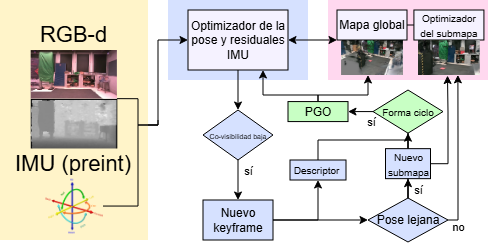
\includegraphics[width=0.9\textwidth]{../imagenes_implementacion/vigs.drawio.png}
    \caption{Los colores azul, rosa y verde representan los hilos de CPU involucrados una vez recibida la entrada de datos al sistema, enmarcada en naranja.}
    \label{fig:diagrama}
\end{figure}

%---------------------------------------------------------
% SECCIONES
%---------------------------------------------------------

\section{Heurísticas para gestión del mapa}

Como ya explicamos, la generación de gaussianas, ya sea en la inicialización o en la densificación, resulta sumamente importante para poder acelerar y corregir la optimización. Debido a que desde un punto de vista teórico no hay una forma cerrada de resolver este problema, se emplean heurísticas como la de FGS-Slam. En esta sección, presentamos otras propuestas que fueron implementadas en este trabajo como sustituto de la de Fourier, basadas en técnicas clásicas del procesamiento de imágenes. Reinterpretamos el problema de la diferenciación de frecuencias como un problema de detección de bordes, donde las regiones de alta frecuencia corresponden a bordes y texturas marcadas.

\subsection{Sobel y Laplace}

A partir del costo computacional adicional asociado a la transformada de Fourier, es natural considerar operadores locales que aproximen el contenido de alta frecuencia sin recurrir a un análisis global del espectro. En este contexto, los operadores de Sobel y Laplace resultan especialmente útiles, ya que permiten detectar cambios bruscos de intensidad de manera simple y eficiente en el dominio espacial.

\textbf{Operador de Sobel.} El operador de Sobel aproxima el gradiente de la imagen, es decir, la primera derivada espacial de la intensidad. Para una imagen $I(x,y)$, las derivadas parciales discretas en las direcciones horizontal y vertical se estiman mediante los kernels:
\begin{equation}
G_x =
\begin{bmatrix}
-1 & 0 & 1 \\
-2 & 0 & 2 \\
-1 & 0 & 1
\end{bmatrix},
\qquad
G_y =
\begin{bmatrix}
-1 & -2 & -1 \\
0 & 0 & 0 \\
1 & 2 & 1
\end{bmatrix}.
\end{equation}
La respuesta de Sobel se obtiene por convolución con la imagen:
\begin{equation}
S_x = I * G_x, \qquad S_y = I * G_y.
\end{equation}
A partir de estas componentes, la magnitud del gradiente se define como:
\begin{equation}
S = \sqrt{S_x^2 + S_y^2}.
\end{equation}
Esta magnitud resalta bordes, texturas y transiciones abruptas, por lo que constituye una aproximación local al contenido de alta frecuencia. A diferencia de Fourier, Sobel no requiere transformar la imagen al dominio frecuencial y su costo computacional es considerablemente menor, lográndose en tiempo lineal.

\textbf{Operador de Laplace.} El operador Laplace aproxima la segunda derivada espacial y, por tanto, mide la variación de la pendiente de la imagen. En dos dimensiones se define como:
\begin{equation}
\nabla^2 I = \frac{\partial^2 I}{\partial x^2} + \frac{\partial^2 I}{\partial y^2}.
\end{equation}
En versión discreta, una aproximación habitual es el kernel:
\begin{equation}
L =
\begin{bmatrix}
0 & 1 & 0 \\
1 & -4 & 1 \\
0 & 1 & 0
\end{bmatrix},
\end{equation}
o variantes equivalentes con conectividad diagonal. Su respuesta se calcula como:
\begin{equation}
L_I = I * L.
\end{equation}
La respuesta del Laplaciano enfatiza cambios rápidos de intensidad en todas las direcciones, por lo que suele destacar bordes finos y estructuras delgadas. Sin embargo, al ser una derivada de segundo orden, también es más sensible al ruido que Sobel. Aunque, del mismo modo, su complejidad temporal es lineal.

\textbf{Construcción de regiones de alta frecuencia.} En nuestra implementación, tanto Sobel como Laplace se utilizan para aproximar la distribución espacial de detalle fino. Una vez obtenida la respuesta de cada operador, se normaliza a $[0,1]$ y se aplica el mismo criterio de umbralización triangular empleado en la heurística de Fourier. Si $M_s$ y $M_l$ denotan las máscaras binarias derivadas de Sobel y Laplace, entonces las regiones de alta frecuencia quedan definidas como:
\begin{equation}
M_s(x,y)=\mathbb{I}[S(x,y)>\tau_s],
\qquad
M_l(x,y)=\mathbb{I}[L(x,y)>\tau_l],
\end{equation}
donde $\mathbb{I}[\cdot]$ es la función indicadora y $\tau_s$, $\tau_l$ son los umbrales estimados por histograma.

\subsection{Canny}

El detector de bordes de Canny constituye una alternativa más estructurada a los operadores diferenciales locales como Sobel y Laplace, ya que incorpora explícitamente un criterio de optimalidad para la detección de bordes: buena detección (baja tasa de falsos negativos), buena localización (bordes bien posicionados) y respuesta única (supresión de múltiples respuestas a un mismo borde).

A diferencia de los métodos basados únicamente en derivadas, Canny introduce un proceso en varias etapas. En primer lugar, la imagen $I(x,y)$ se suaviza mediante un filtro gaussiano para reducir el ruido:
\begin{equation}
I_\sigma(x,y) = I(x,y) * G_\sigma(x,y),
\end{equation}
donde $G_\sigma$ es un kernel gaussiano con desviación estándar $\sigma$.

Luego, se calcula el gradiente de la imagen suavizada:
\begin{equation}
G_x = I_\sigma * G_x^{Sobel}, \qquad G_y = I_\sigma * G_y^{Sobel},
\end{equation}
y su magnitud:
\begin{equation}
G = \sqrt{G_x^2 + G_y^2}.
\end{equation}

A continuación, se aplica supresión de no-máximos, que conserva únicamente los puntos que son máximos locales en la dirección del gradiente, produciendo bordes delgados (típicamente de un solo píxel). Finalmente, se aplica umbralización con histéresis, utilizando dos umbrales $\tau_{low}$ y $\tau_{high}$, definidos como:
\begin{equation}
\tau_{low} < \tau_{high}.
\end{equation}
Los píxeles con gradiente mayor a $\tau_{high}$ se consideran bordes fuertes, mientras que aquellos entre ambos umbrales se conservan únicamente si están conectados a bordes fuertes.

En la implementación utilizada en este trabajo, Canny se aplica directamente sobre la imagen en escala de grises cuantizada a 8 bits. El resultado es una máscara binaria:
\begin{equation}
M_c(x,y) =
\begin{cases}
1, & \text{si } (x,y) \in \text{bordes detectados por Canny}, \\
0, & \text{en otro caso}.
\end{cases}
\end{equation}

A diferencia de Sobel y Laplace, donde la detección de regiones de alta frecuencia depende de un umbral aplicado sobre magnitudes continuas, Canny produce directamente una segmentación binaria basada en un criterio global y contextual de bordes. Esto lo convierte en un detector más preciso y estable frente al ruido, aunque también más restrictivo en términos de densidad de activación.

En el contexto de la densificación de gaussianas, la máscara de Canny puede interpretarse como una estimación de estructura geométrica de la escena. Sin embargo, debido a su naturaleza esquelética (bordes delgados), tiende a subrepresentar regiones texturadas densas que sí son capturadas por Sobel o el análisis espectral de Fourier.


\section{Selección y muestreo de keyframes}
Un problema al tratar con optimización a tiempo real es la cantidad de datos contra el tiempo necesario para procesarlos. La cámara equipada da lugar a un flujo constante de imágenes, llamadas fotogramas o \textit{frames}, de forma tan frecuente que resulta inviable procesarlas todas. Debido a esto, se escogen de forma estratégica qué fotogramas van a ser utilizados para la optimización. Los mismos son llamados fotogramas clave, de ahora en adelante \textit{keyframes}.

La selección de keyframes es categorizada por \cite{robotics12030088} en tres tipos principales: basados en métodos probabilísticos, basados en heurísticas o basados en métodos de aprendizaje.

En el marco de este trabajo, dado un fotograma nuevo se clasifica como keyframe si cumple con un criterio de covisibilidad con el keyframe anterior menor a una cota superior. Esto quiere decir que la información que representa respecto del último keyframe es lo suficientemente nueva.

Para obtener la covisibilidad, se necesita primero calcular la visibilidad estimada de las gaussianas en ambos fotogramas por separado. En cada uno, se identifica qué gaussianas son utilizadas para renderizarlo bajo la representación actual del mundo, observando si su contribución es significativa. Luego, se utiliza una fórmula de Intersección Sobre Unión (Intersection over Union, abreviado IoE) para calcular el ratio:

Sea $G_i$ el conjunto de gaussianas que se consideran visibles,
$$
IoE (G_1, G_2) = \frac{|G_1 \cap G_2|}{|G_1 \cup G_2|} 
$$

Observemos que el denominador no debería anularse, ya que el keyframe anterior debería tener al menos una gaussiana representándolo tras los debidos pasos de optimización.



Ahora, para optimizar sobre ese conjunto de keyframes se toma una muestra que incluya el último. Esto es para no utilizar el conjunto entero, disminuyendo costos de cómputo, pero representando satisfactoriamente el espacio de interés.

Este muestreo se puede realizar de distintos modos, como utilizando distribuciones probabilísticas, tomando siempre los últimos $n$ keyframes o una combinación de ambas, muestreando n con una distribución sobre una ventana de los últimos k keyframes. 



En este trabajo, el muestreo se realizó con una distribución beta-binomial. La misma se define a partir de tres parámetros: $n$, $\alpha$ y $\beta$, y consiste en una distribución binomial de probabilidad $p$, donde $p \sim Beta(\alpha, \beta)$. De este modo, se puede interpretar como muestrear enteros $0$ a $n$ sobre una curva con forma de la distribución beta correspondiente a los parámetros. 

\begin{figure}[H]
    \centering
    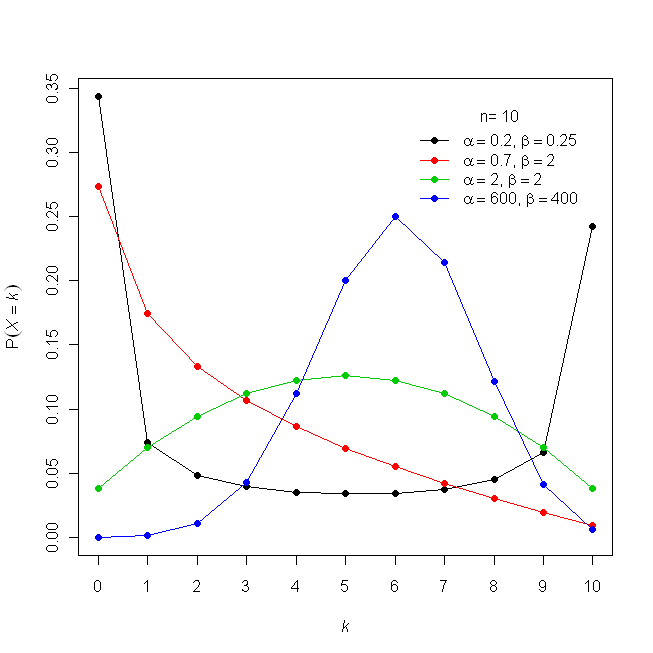
\includegraphics[width=0.8\linewidth]{../imagenes_marco_teorico/Beta-binomial_distribution.png}
    \caption{Distintas combinaciones de $\alpha$ y $\beta$ en la distribución beta binomial para n=10. Con $\alpha = 0.7$ y $\beta=2$ la distribución favorece los valores más bajos con un decaimiento hacia los más altos.}
\end{figure}

\section{Detección y cierre de ciclos}

\subsection{Submapas}

Implementamos el sistema de submapas propuesto en LoopSplat, realizando todas las operaciones que antes eran globales, como la optimización de las gaussianas en la imagen, en un marco local de cada submapa. De esta forma, cada submapa se construye a partir de un conjunto de fotogramas consecutivos, obteniendo así regiones reducidas. Si bien esto beneficia la eficiencia de las operaciones, reduce la ventaja del muestreo global de keyframes, ya que dos keyframes de submapas distintos no pueden ser comparados directamente. Esto quiere decir que la optimización pierde el mantenimiento global por sí sola. Sin embargo, en este marco el objetivo es el mantenimiento global a partir de los ciclos, enriqueciendo no solo la calidad de la representación, sino también la estimación de la pose.

\subsection{Descriptor}

Para la extracción del descriptor NetVLAD utilizamos la implementación en Python de HLoc \cite{sarlin2019coarse}, disponible en \url{https://github.com/cvg/Hierarchical-Localization} y la red preentrenada en el conjunto de datos Pitts30k, de forma análoga a LoopSplat. Esta versión de la red da lugar a descriptores de tamaño $4096$. Como nuestra implementación está escrita en C++, la integración con HLoc se realiza montando un servidor que contiene el código de extracción en Python. El cliente, es decir nuestro nodo, se comunica con el servidor entregándole la imagen a procesar y recibiendo el descriptor.

Esta implementación añade tiempos de latencia adicionales debido a los tiempos de comunicación, sin embargo, la arquitectura desacoplada de los hilos de detección de ciclos y el modelo de procesamiento por submapas permiten que esta latencia no afecte negativamente el rendimiento general del sistema. Además, facilita el acceso a posibles mejoras futuras en la red NetVLAD sin necesidad de reimplementaciones.

Es posible implementar este factor en un nodo separado de ROS2, realizando la comunicación a través de mensajes. Sin embargo, esto mantiene la latencia de comunicación, y abre la posibilidad de incompatibilidades entre las versiones de Python y dependencias entre ROS2 y HLoc. Por ello, se optó por una comunicación directa que, a su vez, permite optimizaciones en GPU.

\subsection{Heurísticas la detección de ciclos}

Para reducir el número de falsos positivos en la detección de ciclos, se implementan dos heurísticas principales. La primera es un filtro basado en la coherencia entre los centros de los submapas candidatos: si la distancia euclidiana entre los centros de las nubes de puntos de los submapas es mayor que un umbral predefinido, se descarta la correspondencia. Análogamente, si la orientación entre dos submapas no es coherente, también se descarta. La segunda heurística es el filtro por similaridad definido en el trabajo original.


\subsection{Registro de gaussianas}

En lugar de utilizar un método basado en los jacobianos de la renderización, optamos por un enfoque más clásico en SLAM basado en el registro de nubes de puntos. Para ello, reinterpretamos los centros de las gaussianas como puntos en el espacio 3D, y sus covarianzas como incertidumbres asociadas a cada punto. De esta forma, el problema de registro se convierte en un problema de alineación de nubes de puntos. Para resolverlo, empleamos una variante de ICP (\textit{Iterative Closest Point}) que tiene en cuenta las covarianzas, implementada en Open3D \cite{zhou2018open3dmodernlibrary3d}. Esta librería requiere una estimación inicial de la transformación, la cual obtenemos a partir de la pose estimada por la IMU.

\subsection{Optimización del grafo de poses}

Una vez obtenidas las correspondencias entre los submapas que cierran un ciclo, se construye un grafo de poses donde cada nodo representa la pose de un submapa y cada arista representa una restricción de transformación. Para optimizar este grafo, se utiliza la biblioteca Ceres Solver \cite{Agarwal_Ceres_Solver_2022}, que permite resolver problemas de optimización no lineal en CPU. Debido a la reducción del número de nodos como submapas, la optimización no se ve afectada significativamente por el rendimiento de la CPU.

\section{ROS2}

El programa desarrollado en este trabajo se implementó utilizando ROS2 (Sistema Operativo de Robots 2), que es una plataforma de software de código abierto ampliamente utilizada en actividades de robótica. 

ROS2 proporciona una infraestructura de comunicación entre procesos mediante un modelo de publicación y suscripción. La idea general es que los programas se organizan en nodos, que son procesos independientes que pueden comunicarse entre sí por medio de mensajes. Un nodo puede publicar mensajes en lo que se llama tópicos, que son fundamentalmente un canal de comunicación por el que transfiere un tipo de dato. Por otro lado, un nodo puede suscribirse a un tópico, lo que significa que recibirá los mensajes publicados allí. De este modo, los nodos intercambian información manteniendo la modularidad e independencia. La forma en la que se recibe un mensaje es mediante una función callback, que es una función que se ejecuta cada vez que un mensaje llega al tópico al que el nodo está suscrito.

\begin{figure}[H]
    \centering
    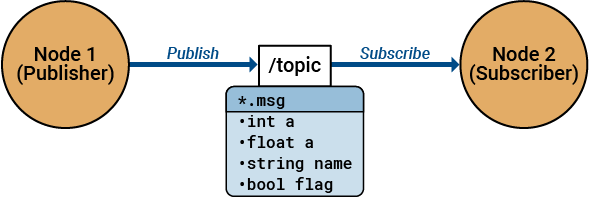
\includegraphics[width=0.8\linewidth]{../imagenes_implementacion/What-is-a-ROS2-message.png}
    \caption{Idea general de cómo funcionan los mensajes en ROS2. El nodo 1 publica mensajes en un tópico, cada mensaje con ciertos datos. El nodo 2, por su parte, se suscribe al tópico. Así, cada vez que el nodo 1 publique algún dato, el callback asociado en el nodo 2 se ejecutará. Imagen extraida de \cite{mathworks_ros2_topics}}
    \label{ros2_message}
\end{figure}

Dentro de este marco, los conjuntos de datos preparados para probar el programa funcionan como un nodo que publica los datos recopilados en los tópicos correspondientes siguiendo los tiempos originales. Es decir, funciona de forma similar a un vídeo, el cual está grabado y podemos reproducir a tiempo real cuando queramos.

Una de las limitaciones principales de ROS2 es que no posee ningún tipo de optimización para el procesamiento en GPU, esto quiere decir que el manejo de mensajes y nodos se realiza exclusivamente en CPU. De este modo, un factor limitante para la implementación es que los mensajes principales y las funciones asociadas tienen que organizarse tal que la recepción y el envío de datos resida en la memoria y en las instrucciones de la CPU.

El programa principal, contenido en un nodo, recibe como entradas los siguientes parámetros: información de la IMU, intrínsecas de las cámaras, imágenes RGB e imágenes de profundidad, estas últimas alineadas al marco de la cámara RGB. Sin embargo, no todos los conjuntos de datos cuentan con las imágenes de profundidad alineadas, por lo que, además, se implementó un nodo adicional que se encarga de registrar las imágenes, publicando así las imágenes de profundidad alineadas. Este nodo está programado en GPU, por lo que su costo es mínimo.

Como salida, el programa publica la pose estimada del robot, así como una ventana que permite visualizar el mapa reconstruido en tiempo real.







\section{Tareas en GPU}

La implementación de los filtros Sobel y Laplace es directamente paralelizable procesando cada píxel por separado. Para Fourier y Canny utilizamos librerías de NVIDIA, que ya están optimizadas para GPU.

Para el renderizado, trabajamos con una técnica estándar en este tipo de algoritmo que es el basado en tiles (o mosaicos). En esta técnica, la imagen de salida se divide en regiones de tamaño fijo, en este caso $16 \times 16$ píxeles, y cada región es procesada por un bloque de hilos en la GPU. Cada hilo dentro del bloque se encarga de calcular la contribución de las gaussianas a un píxel específico dentro de esa región. El motivo de emplear esta división es que las gaussianas contribuyen de forma significativa a un área limitada de la imagen, por lo que los píxeles de una misma región comparten muchas de las gaussianas, mientras que para regiones separadas las gaussianas relevantes varían. Así, podemos descartar muchas gaussianas según su distancia a la región, reduciendo los cálculos necesarios por píxel y aprovechando la memoria compartida del bloque para las gaussianas involucradas.

Para las jacobianas, y el resto de operaciones relacionadas, trabajamos con un hilo por gaussiana, donde el resultado numérico se acumula en la memoria global antes de ser pasado a la CPU. De este modo, y al igual que en VIGS-Fusion, la CPU solo trabaja con matrices de tamaño reducido.





\section{Hilos en CPU}

La CPU, de forma similar a la GPU, también puede ejecutar tareas en paralelo mediante el uso de hilos. Un hilo es una unidad de ejecución dentro de un proceso, y permite que diferentes partes de un programa se ejecuten simultáneamente. En este trabajo, se utilizan hilos en CPU para gestionar tareas que pueden ejecutarse con cierto grado de paralelismo pero que no requieren la potencia de una GPU ni cumplen el principio SIMD, es decir, no es posible dividirlas en partes pequeñas. Además, los hilos en CPU permiten trabajar en tareas con recursos compartidos donde los hilos se bloquean mutuamente para evitar conflictos, teniendo un sentido de orden en la ejecución.

\subsection{Hilos empleados}

Las tareas relacionadas a la localización, así como la gestión de keyframes y funciones principales, se realizan en un hilo dedicado. Esto se debe a que estas tareas requieren un orden específico y secuencial que determina el flujo de ejecución. En este hilo se encuentra la función que recibe las imágenes y la información de la IMU organizadas, encargándose tanto de la toma de decisiones (por ejemplo, si tratarla como un nuevo keyframe o no) como de la ejecución de las funciones necesarias para actualizar la pose a partir del problema de minimización. Este problema se resuelve utilizando la biblioteca Ceres, que permite resolver problemas de optimización no lineal de forma eficiente, exclusiva de CPU.

Por otro lado, un hilo distinto se encarga de optimizar el mapa, es decir, actualizar los parámetros de las gaussianas. Aquí se muestrea dentro del submapa, y luego se realiza la optimización con ADAM en GPU. De este modo, comparte con el hilo principal la información de las gaussianas, pero se bloquean cuando es necesario para evitar colisiones.

Un tercer hilo se encarga de la visualización, actualizando la ventana que muestra el mapa reconstruido en tiempo real así como las poses estimadas. Este hilo no participa en el sistema principal, sino que funciona únicamente para mostrar la información.

Del mismo modo que LoopSplat \cite{zhu2025_loopsplat}, separamos las tareas relacionadas a los ciclos en un hilo dedicado para evitar bloqueos. Así, un cuarto hilo se encarga del proceso completo de detección, verificación, registro y cierre de ciclos. Este hilo trabaja exclusivamente sobre los submapas cerrados, por lo que apenas colisiona con los hilos principales.


%=========================================================

%%%%%%%%%%%%%%%%%%%%%%%%%%%%%%%%%%%%%
% RESULTADOS
%%%%%%%%%%%%%%%%%%%%%%%%%%%%%%%%%%%%%
%=========================================================
% CAPÍTULO: Resultados
%=========================================================

\chapter{Resultados}
\label{resultados}


\wip{TERMINAR}

%---------------------------------------------------------
% SECCIONES
%---------------------------------------------------------

\section{Métricas}

Para evaluar el desempeño del sistema se utilizan métricas clásicas en SLAM que permiten analizar tanto la calidad de la estimación de trayectoria como la calidad de la reconstrucción visual y el costo computacional asociado. En particular, se reportan las métricas ATE RMSE, PSNR, tiempo de mapeo por imagen (\textit{Map/img}) y tiempo de seguimiento por imagen (\textit{Track/img}).

\subsection{ATE RMSE}

El \textit{Absolute Trajectory Error Root Mean Square Error} (ATE RMSE) mide la precisión de la trayectoria estimada respecto de una trayectoria de referencia (\textit{ground truth}). Para ello, se compara la posición estimada de la cámara en cada instante con la posición real correspondiente.

Sea $\mathbf{p}_i$ la posición estimada y $\mathbf{p}_i^{gt}$ la posición de referencia para el instante $i$. El error absoluto de trayectoria se define como:

$$
e_i = \left| \mathbf{p}_i - \mathbf{p}_i^{gt} \right|.
$$

A partir de estos errores individuales, el ATE RMSE se calcula como:

$$
\mathrm{ATE}_{RMSE}
=
\sqrt{
\frac{1}{N}
\sum_{i=1}^{N}
e_i^2
},
$$

donde $N$ es la cantidad de poses evaluadas.

Esta métrica cuantifica el error global acumulado de la trayectoria. Valores menores indican una mejor estimación de la pose y una menor deriva durante la navegación.

\subsection{PSNR}

El \textit{Peak Signal-to-Noise Ratio} (PSNR) evalúa la calidad visual de las imágenes renderizadas a partir del mapa reconstruido comparándolas con las imágenes reales capturadas por la cámara.

Su definición se basa en el error cuadrático medio (MSE):

$$
\mathrm{MSE}
=
\frac{1}{HW}
\sum_{u=1}^{H}
\sum_{v=1}^{W}
\left(
I(u,v)-\hat{I}(u,v)
\right)^2,
$$

donde:

\begin{itemize}
\item $I(u,v)$ es el valor del píxel de la imagen de referencia.
\item $\hat{I}(u,v)$ es el valor del píxel renderizado.
\item $H$ y $W$ representan la altura y el ancho de la imagen.
\end{itemize}

A partir del MSE, el PSNR se define como:

$$
\mathrm{PSNR}
=
10 \log_{10}
\left(
\frac{L^2}{\mathrm{MSE}}
\right),
$$

donde $L$ es el valor máximo posible de intensidad de un píxel.

El PSNR se expresa en decibeles (dB). Valores más altos indican una reconstrucción visual más fiel a las observaciones originales.

\subsection{Tiempo de mapeo por imagen (Map/img)}

La métrica \textit{Map/img} mide el tiempo promedio dedicado a la etapa de mapeo para cada imagen procesada.

Esta etapa incluye operaciones como la incorporación de nuevos keyframes, la optimización de gaussianas y las actualizaciones de la representación del mapa.

Se calcula como:

$$
\mathrm{Map/img}
=
\frac{T_{\mathrm{map}}}{N},
$$

donde $T_{\mathrm{map}}$ es el tiempo total invertido en tareas de mapeo y $N$ es la cantidad de imágenes procesadas.

Esta métrica permite evaluar el costo computacional asociado al mantenimiento y refinamiento del mapa.

\subsection{Tiempo de seguimiento por imagen (Track/img)}

La métrica \textit{Track/img} mide el tiempo promedio requerido para estimar la pose de la cámara a partir de cada nueva observación.

Incluye las operaciones realizadas durante la etapa de seguimiento, tales como el renderizado necesario para la estimación de pose y la optimización asociada.

Se define como:

$$
\mathrm{Track/img}
=
\frac{T_{\mathrm{track}}}{N},
$$

donde $T_{\mathrm{track}}$ representa el tiempo total dedicado al seguimiento y $N$ la cantidad de imágenes procesadas.

Esta métrica resulta particularmente relevante para evaluar la capacidad del sistema de operar en tiempo real, ya que determina la latencia asociada a la estimación de pose.


\section{Conjunto de datos}

Para evaluar el desempeño del sistema, utilizamos el conjunto de datos propuesto en el mismo artículo de VIGS-Fusion \cite{ndoye2025vigs}, disponible en \url{https://entrepot.recherche.data.gouv.fr/dataset.xhtml?persistentId=doi:10.57745/CI0K9G}. Este conjunto de datos se compone de secuencias de video capturadas en un entorno interior, con una cámara RGB-D y una IMU. Las secuencias incluyen movimientos variados, así como las trayectorias de referencia obtenidas mediante un sistema de seguimiento externo. Actualmente, es el único conjunto de datos público que incluye tanto imágenes RGB-D como datos de IMU calibrados.

En particular, las métricas fueron tomadas sobre las siguientes secuencias:

\begin{enumerate}
    \item \textit{Line}: Secuencia con un movimiento lineal del UAV. Luego de comenzar, se eleva, se desplaza hacia adelante, vuelve y aterriza donde comenzó
    \item \textit{Square-Shape}: Secuencia con un movimiento en forma de cuadrado. Se eleva, se desplaza hacia delante, gira 90 grados y repite el proceso hasta volver al punto de inicio, donde aterriza.
    \item \textit{Rotation-Only}: Secuencia donde se eleva, realiza un giro de 360 grados y luego aterriza en el inicio.
    \item \textit{Line-Rot}: Similar a la secuencia \textit{Line}, pero luego de desplazarse hacia delante realiza rotaciones hacia ambos lados antes de volver.
\end{enumerate}

\section{Evaluación}

\subsection{Comparativa entre heurísticas de gestión de mapa}

En la Figura \ref{fig:mascaras_original} se muestra un ejemplo de una imagen correspondiente al conjunto de datos empleado para evaluar el trabajo. Podemos observar que hay superficies planas, telas levemente arrugadas y algunas cajas con texturas.

\begin{figure}[H]
    \centering
    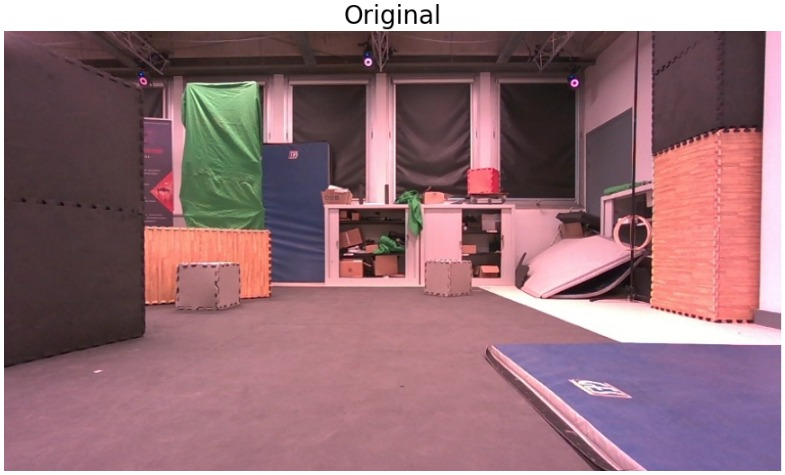
\includegraphics[width=0.7\linewidth]{../imagenes_implementacion/mascaras_original.png}
    \caption{Primera imagen de la secuencia \textit{Line} del conjunto de datos \textit{VIGS-Fusion}.}
    \label{fig:mascaras_original}
\end{figure}

Ahora, en la Figura \ref{fig:masks} se presentan las máscaras obtenidas por cada una de las heurísticas implementadas. Se puede apreciar que la máscara de Fourier genera bordes gruesos y es más sensible a zonas de alta variación de frecuencia, como el fondo de la imagen. Sobel, por su lado, genera bordes gruesos y un poco más sensibles a las texturas, aunque con más precisión para las zonas de alta variación. Laplace, en cambio, es muy sensible al ruido, generando bordes menos definidos. Finalmente, Canny produce bordes delgados y bien definidos, pero con una cobertura mucho menor, especialmente es zonas texturadas, lo que puede resultar en una máscara demasiado escasa para guiar la densificación de gaussianas de manera efectiva.

\begin{figure}[H]
    \centering

    \begin{subfigure}{0.48\textwidth}
        \centering
        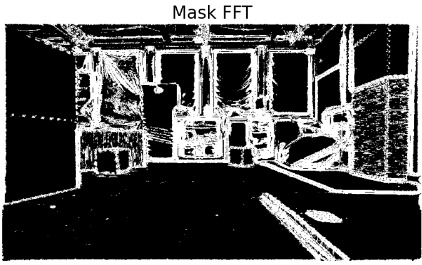
\includegraphics[width=\linewidth]{../imagenes_implementacion/mask_fft.png}
        \caption{FFT}
    \end{subfigure}
    \hfill
    \begin{subfigure}{0.48\textwidth}
        \centering
        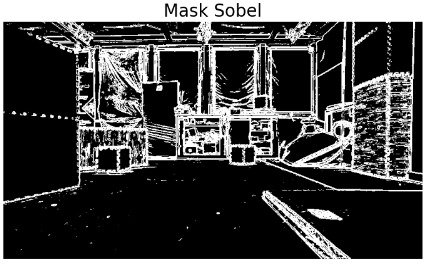
\includegraphics[width=\linewidth]{../imagenes_implementacion/mask_sobel.png}
        \caption{Sobel}
    \end{subfigure}

    \vspace{0.5em}

    \begin{subfigure}{0.48\textwidth}
        \centering
        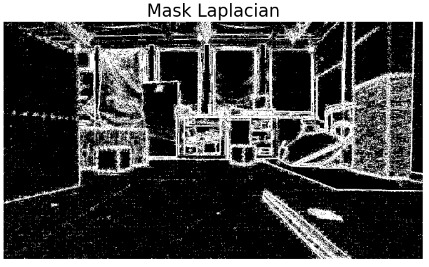
\includegraphics[width=\linewidth]{../imagenes_implementacion/mask_laplace.png}
        \caption{Laplace}
    \end{subfigure}
    \hfill
    \begin{subfigure}{0.48\textwidth}
        \centering
        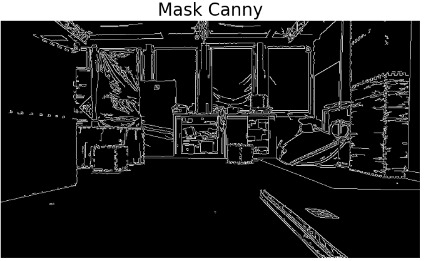
\includegraphics[width=\linewidth]{../imagenes_implementacion/mask_canny.png}
        \caption{Canny}
    \end{subfigure}

    \caption{Comparación de máscaras obtenidas mediante distintos métodos.}
    \label{fig:masks}
\end{figure}

Luego, comparamos las métricas fijando un conjunto de datos.

\begin{table}[H]
\centering
\caption{Comparación de funciones de selección de keyframes sobre la secuencia \textit{Line}.}
\label{tab:line_ablation}
\begin{tabular}{lcccc}
\hline
\textbf{Método} & \textbf{Track/img [ms]} & \textbf{Map/img [ms]} & \textbf{PSNR [dB]} & \textbf{ATE RMSE} \\
\hline
F [VIGS]      & 49.71 & 8.92  & 21.44 & 9.12 \\
F [Fourier]   & 50.23 & 12.09 & 28.13 & 9.54 \\
F [Canny]     & 53.58 & 9.89  & 26.11 & 9.02 \\
F [Sobel]     & 52.02 & 9.21  & 27.81 & 8.87 \\
F [Laplacian] & 52.95 & 11.96 & 27.92 & 8.95 \\
\hline
\end{tabular}
\end{table}

En la tabla \ref{tab:line_ablation} podemos observar que el uso de máscaras de frecuencia mejora la calidad visual sin un costo añadido significativo. En particular, el método basado en Sobel logra un PSNR de 27.31 dB sin tener un impacto costoso en los tiempos, mientras que Fourier logra un PSNR de 28.13 dB, siendo el de mayor calidad, pero con un costo de mapeo más elevado.

Debido a que la gestión de mapa funciona a partir de un muestreo fino en las zonas de alta frecuencia, y uno más espaciado en las de baja, es esperable que los métodos que capturan una mayor región de la imagen logren un mejor PSNR. Sin embargo, debido a que buscamos un método para uso a tiempo real, tomamos el balance entre calidad y costo y empleamos en el resto del trabajo Sobel.

\subsection{Comparativa con VIGS-Fusion}

A continuación, presentamos una comparativa evaluando nuestro nodo y el de VIGS-Fusion utilizando el conjunto de datos mencionado. Para cada secuencia, se evalúan las métricas ejecutando a tiempo real, es decir, perdiendo todos los fotogramas que no llegan a procesarse. Los resultados se resumen en la Tabla \ref{tab:results_comparison}. Las secuencias que poseen ciclos poseen un único ciclo justo al final, y son \textit{Square-Shape} y \textit{Rotation-Only}. Las métricas fueron tomadas con una GPU NVIDIA RTX 3090 y una CPU Intel i5-9400F.


\begin{table}[H]
\centering
\caption{Comparación de métricas entre la configuración propuesta y VIGS-Fusion.}
\label{tab:results_comparison}
\begin{tabular}{llcccc}
\hline
\textbf{Dataset} & \textbf{Método} & \textbf{Track [ms]} & \textbf{Map [ms]} & \textbf{PSNR [dB]} & \textbf{ATE} \\
\hline
                % TRACK % MAP % PSNR % ATE
\multirow{2}{*}{Line}
& Nuestro       & 52.02 & 9.41 & 27.51 & 8.87 \\
& VIGS-Fusion  & 56.35  & 12.32 & 22.19& 9.95 \\
\hline

\multirow{2}{*}{Square-Shape}
& Nuestro       & 57.93 & 15.19 & 24.28 & 16.73 \\
& VIGS-Fusion  & 54.49  & 19.50 & 22.19& 21.52     \\
\hline

\multirow{2}{*}{Rotation-Only}
& Nuestro       & 42.11 & 10.38 & 25.08 & 18.84 \\
& VIGS-Fusion  & 39.91   & 17.11 & 20.31 & 24.95     \\
\hline

\multirow{2}{*}{Line-Rot}
& Nuestro       & 43.73 & 7.67 & 25.77 & 11.16 \\
& VIGS-Fusion  & 48.02  & 9.89 & 18.59  & 11.82      \\
\hline

\end{tabular}
\end{table}

\subsection{Visualización}

A continuación, se presentan algunas visualizaciones de los resultados obtenidos por nuestro método. En aquellas visualizaciones donde se pueda observar el recorrido, se muestra únicamente la posición de los keyframes y submapas, sin mostrar la trayectoria estimada en todo momento. De este modo podemos apreciar los criterios de selección de keyframes y de inicio de submapas. Es importante tener en cuenta que la trayectoria sigue la información de la IMU entre keyframe y keyframe, recibiendo correcciones de la cámara únicamente en los keyframes, por ello es importante que los mismos estén bien distribuidos.

\begin{figure}[H]
    \centering

    \begin{subfigure}{0.49\textwidth}
        \centering
        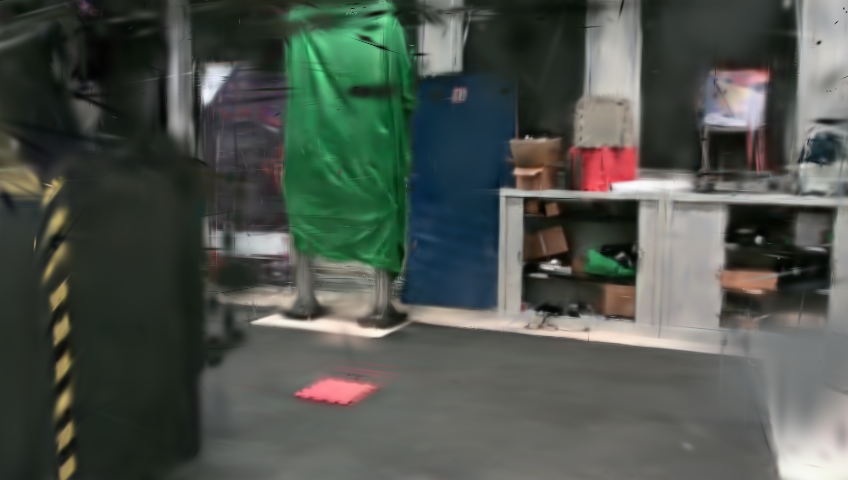
\includegraphics[width=\linewidth]{../imagenes_resultados/ejemplo_1.png}
        \caption{Mapa visto desde el recorrido.}
        \label{fig:ejemplo_izq1}
    \end{subfigure}
    \hfill
    \begin{subfigure}{0.49\textwidth}
        \centering
        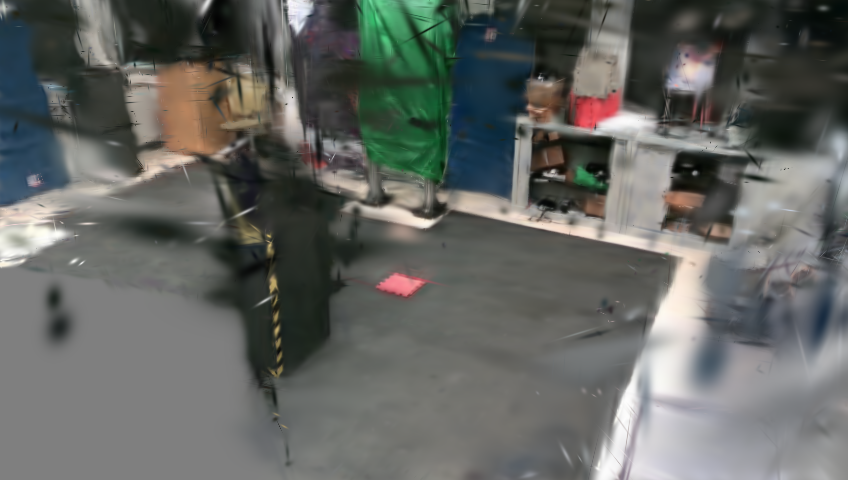
\includegraphics[width=\linewidth]{../imagenes_resultados/ejemplo_3.png}
        \caption{Mapa desde una posición distinta.}
        \label{fig:ejemplo_der1}
    \end{subfigure}

    \caption{Se observa cómo podemos navegar la reconstrucción del mapa más allá de adherirnos al recorrido del robot.}
    \label{fig:comparacion1}
\end{figure}

\begin{figure}[H]
    \centering

    \begin{subfigure}{0.49\textwidth}
        \centering
        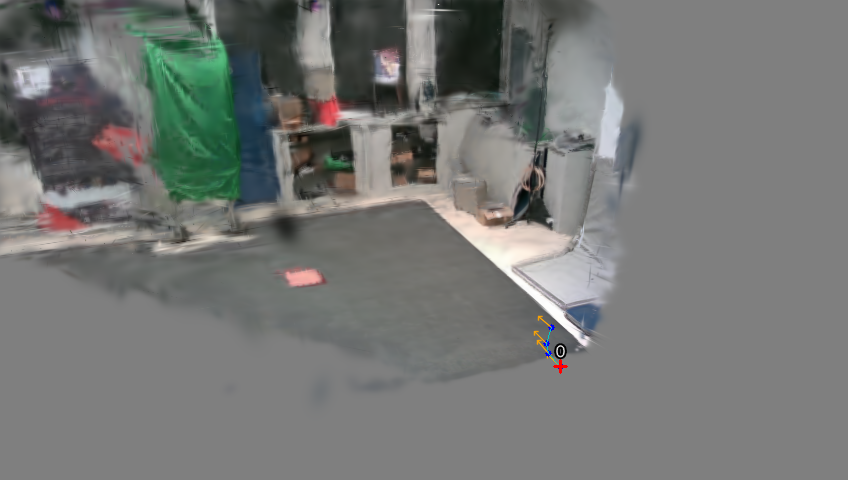
\includegraphics[width=\linewidth]{../imagenes_resultados/ejemplo2_1.png}
        \caption{Inicio del mapa.}
        \label{fig:ejemplo_izq2}
    \end{subfigure}
    \hfill
    \begin{subfigure}{0.49\textwidth}
        \centering
        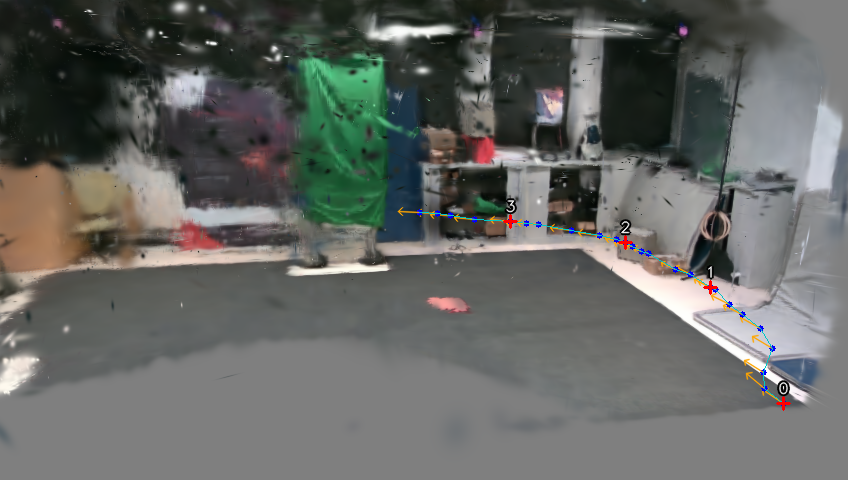
\includegraphics[width=\linewidth]{../imagenes_resultados/ejemplo2_2.png}
        \caption{Continuación del mapa.}
        \label{fig:ejemplo_der2}
    \end{subfigure}

    \caption{Cada cruz roja numerada es el inicio de un submapa, donde cada punto azul es un keyframe del mismo. Se observa cómo el mapa se va reconstruyendo a medida que el robot avanza.}
    \label{fig:comparacion2}
\end{figure}

\begin{figure}[H]
    \centering

    \begin{subfigure}{0.49\textwidth}
        \centering
        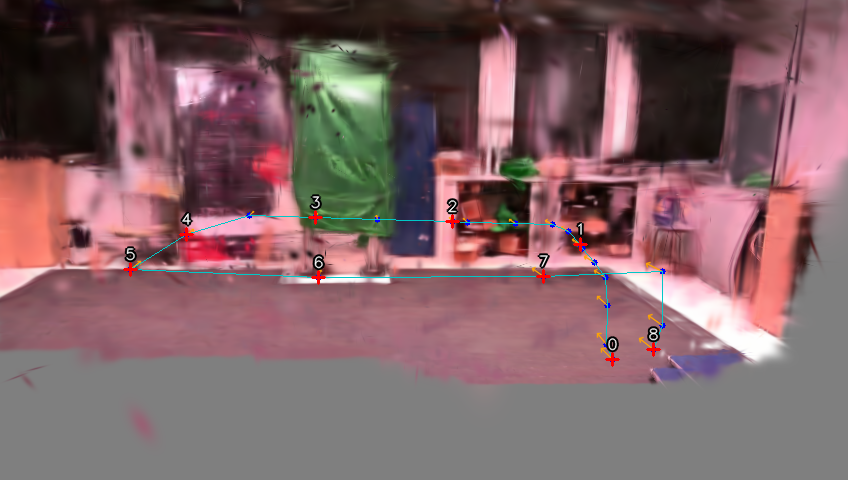
\includegraphics[width=\linewidth]{../imagenes_resultados/ejemplo3_1.png}
        \caption{Mapa sin cierre de ciclos.}
        \label{fig:ejemplo_izq3}
    \end{subfigure}
    \hfill
    \begin{subfigure}{0.49\textwidth}
        \centering
        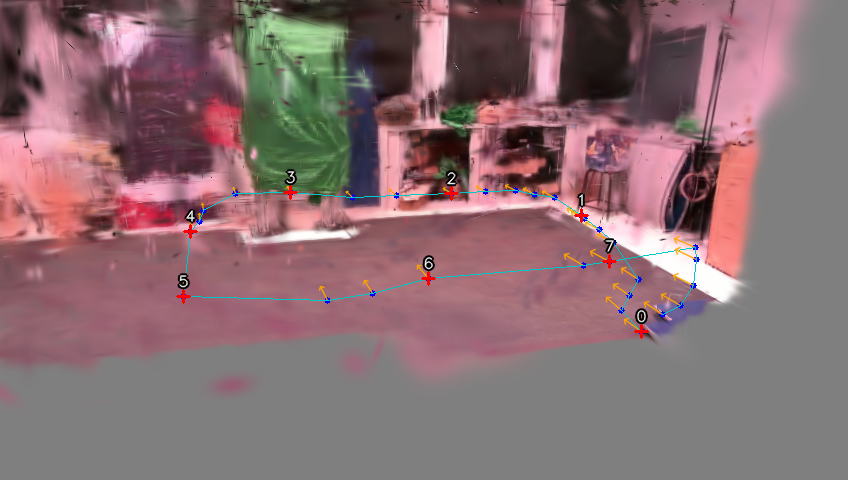
\includegraphics[width=\linewidth]{../imagenes_resultados/ejemplo3_2.png}
        \caption{Mapa con cierre de ciclos.}
        \label{fig:ejemplo_der3}
    \end{subfigure}

    \caption{La secuencia \textit{Square-Shape} posee un ciclo al final del recorrido. En la imagen de la izquierda se observa el mapa sin aplicar cierre de ciclos, donde se puede apreciar una desviación acumulada que genera una discontinuidad en el mapa. En la imagen de la derecha, al aplicar cierre de ciclos, se corrige esta desviación y se obtiene un recorrido consistente.}
    \label{fig:comparacion3}
\end{figure}

%=========================================================

%%%%%%%%%%%%%%%%%%%%%%%%%%%%%%%%%%%%%
% CONCLUSIONES
%%%%%%%%%%%%%%%%%%%%%%%%%%%%%%%%%%%%%
\chapter{Conclusiones}
\label{conclusiones}

En este trabajo se presentó una extensión de un sistema de SLAM visual-inercial basado en Gaussian Splatting, incorporando variaciones en la gestión de mapa y la detección y cierre de ciclos. El objetivo principal fue obtener un sistema más robusto y preciso, capaz de aprovechar el recorrido para corregir los errores en la deriva y mejorar la calidad de la estimación y el modelo de mapa.

Para ello, se desarrolló una variante del sistema original de VIGS-Fusion con: un preprocesamiento de las imágenes para mejorar la gestión del mapa de gaussianas basado en regiones de alta frecuencia, un modelo de submapeo para mejorar la eficiencia computacional, una estrategia de detección de ciclos a partir de descriptores NetVLAD, y un proceso de optimización global para la corrección de la trayectoria y el mapa al detectar un ciclo.

Los resultados obtenidos en los experimentos muestran que el preprocesamiento de las imágenes es un proceso con un costo negligible que mejora la calidad de la reconstrucción visual, y que el modelo de submapeo reduce el costo computacional sin afectar la calidad de la estimación. Además, en los conjuntos de datos evaluados, aquellos con algún ciclo presentaron una mejora significativa en las métricas, mientras que aquellos sin ciclos no presentaron un empeoramiento..

\section{Trabajo futuro}

Como trabajo futuro, un camino que consideramos importante es la exploración de otros conjuntos de datos como EuRoC-MAV \cite{eurocmav}, que presenta secuencias con una duración más larga, así como algunas con más ciclos, permitiendo evaluar el desempeño del sistema en escenarios más complejos. Sin embargo, este conjunto de datos no incluye datos de una cámara de profundidad sino de una cámara estéreo, por lo que sería necesario preprocesar las imágenes mediante un método de estimación de la profundidad.

Además, un cuello de botella en la implementación actual fue la dependencia total de ROS2, lo que imposibilitó optimizaciones al introducir limitaciones a través de la CPU. En este sentido, se puede explorar una implementación desacopladas que permita, además, comparar el trabajo con otros sistemas de Gaussian Splatting que no estén integrados en ROS2 y extender sus posibles usos. 


\newpage

\backmatter
\bibliographystyle{unsrt}
\bibliography{tesis}

\end{document}
